% don't remove the folling lines, and edit the defintion of \main if needed
\documentclass[../report.tex]{subfiles}
\providecommand{\main}{..}
\IfEq{\jobname}{\currfilebase}{\AtEndDocument{\biblio}}{}
% until here

\begin{document}

\section{Di-Higgs production and Higgs self couplings\label{sec3}}

The HL-LHC is expected to be a Higgs boson factory, and the study of the double-Higgs ($HH$) production is one of the key goal of this high-luminosity program. Despite the small production cross-section compared to the single-Higgs boson production, more than 100000 $HH$ should be produced by the HL-LHC per experiment. The trilinear self-interaction of the Higgs boson is described by a with a coupling strength $\lambda_{HHH}  = \frac{m_H^2}{2v^2} $, where $m_H$ is the Higgs boson mass, and $v$ the electroweak symmetry breaking vacuum expectation value. Measurements of the Higgs trilinear interaction would provide constraints on the shape of the Higgs potential close to the minimum. and would allow to verify the electroweak symmetry breaking mechanism of the SM.
The existence of an extended scalar sector or the presence of new dynamics at higher scales could modify the Higgs boson self-couplings.
In the following the trilinear self-coupling strength, measured relative to the SM expectation is denoted by $\kappa_{\lambda} = \lambda_{HHH}/\lambda_{HHH}^{SM}$

This section describes the prospects for studies of the Higgs boson pair production at the HL-LHC and HE-LHC and is organised as follows: the state-of-the-art NLO computions of the Higgs boson pair production cross sections is shown in Section~\ref{sec:HH_NLO}. Section~\ref{sec:HH_meas_exp} describes the prospect experimental analyses with the ATLAS and CMS experiments with realistic conditions, while Section~\ref{sec:HH_meas_th} concentrates on alternative methods with phenomenology studies. Studies at the HE-LHC are shown in Section~\ref{sec:HH_HE} with both phenomenological and experimental perspectives. Indirect probes of the trilinear couplings are described in Section~\ref{sec:HH_indirect}, using differential cross-section measurements or global fits. Finally Section~\ref{sec:HH_implications} show the implications of the trilinear coupling measurements on b-physics and the electroweak phase transition.  

\subsection{Higgs boson pair production cross section}
\label{sec:HH_NLO}

\subsubsection{SM Calculation}

\subsubsubsection{HH production at NNLO}
\begin{center}
    \textit{by Javier Mazzitelli}
\end{center}

The fusion of gluons via a heavy-quark (mainly top-quark) loop is the most important production mechanism of Higgs boson pairs at hadron colliders within the SM.
The NLO QCD corrections for this process have been known in the large-$m_t$ limit for some time \cite{Dawson:1998py}, and the NNLO cross section has also been computed within this approximation \cite{deFlorian:2013jea}.
The NLO corrections retaining the full dependence on the top-quark mass have been obtained for the first time in Refs.~\cite{Borowka:2016ehy,Borowka:2016ypz}, and have been recently confirmed by an independent calculation \cite{Baglio:2018lrj}.
On top of this, an improved NNLO prediction --labeled NNLO$_{\mathrm{FTa}}$ for full-theory approximation-- was presented in Ref.~\cite{Grazzini:2018bsd}.
This approximation is obtained by combining one-loop double-real corrections with full $m_t$ dependence with suitably reweighted real-virtual and double-virtual contributions evaluated in the large-$m_t$ limit.
Furthermore, the stability of the QCD perturbative expansion at this order has been confirmed by consistently matching the NNLO$_{\mathrm{FTa}}$ prediction with the next-to-next-to-leading logarithmic terms coming from threshold resummation \cite{deFlorian:2018tah}.

More details on the NLO results with full-$m_t$ dependence (including the effect coming from variations in the Higgs self-coupling and the contributions arising from BSM EFT operators) are provided in the following sections, therefore we focus here on the state-of-the-art NNLO prediction, i.e., the NNLO$_{\mathrm{FTa}}$ result from Ref.~\cite{Grazzini:2018bsd}.

Before focusing on the numerical results, it is worth to stress out that the NNLO cross sections presented here, as well as the NLO predictions for gluon fusion present in the following sections, are computed using the on-shell scheme for the top-quark mass renormalization.
Some partial results on the uncertainties related to the $m_t$ scheme and scale choice have been presented in Ref.~\cite{Baglio:2018lrj} at NLO, and further studies to gauge the size of their effect on the total cross section and distributions are in progress.
This source of uncertainty is for the moment not considered in the NLO and NNLO predictions.

In Table \ref{table:HH_at_NNLO} we present results for the total cross section at $\sqrt{s} = 14$~TeV and 27~TeV.
We use the values $m_h = 125$~GeV for the Higgs boson mass and $m_t = 173$~GeV for the  on-shell top quark mass.
The NNLO PDF4LHC15 sets of parton distribution functions are used, and PDF and $\alpha_S$ uncertainties are also provided.
An estimation of the systematic uncertainty of the approximation due to missing finite-$m_t$ effects is also presented, and it is found to be at the few percent level.
For the renormalization and factorization scales we use the central value $\mu_0 = M_{hh}/2$, which has been shown to provide a better convergence for the fixed order prediction \cite{deFlorian:2018tah}. We obtain the scale uncertainties via the usual 7-point scale variation.

%%====================================
{\renewcommand{\arraystretch}{1.6}
\begin{table}
\begin{center}
\begin{tabular}{|l|c|c|c|c|c|}
\hline
$\sqrt{s}$~[TeV] & NNLO$_{\mathrm{FTa}}$~[fb] & $m_t$ unc. & PDF unc. & $\alpha_S$ unc. & PDF$+\alpha_S$ unc. \\
 \hline
$14$ & $36.69^{+2.1\%}_{-4.9\%}$ & $\pm 2.7\%$ & $\pm 2.1\%$ & $\pm 2.1\%$ & $\pm 3.0\%$ \\
\hline
$27$ & $139.9^{+1.3\%}_{-3.9\%}$ & $\pm 3.4\%$ & $\pm 1.7\%$ & $\pm 1.8\%$ & $\pm 2.5\%$ \\
\hline
\end{tabular}
\end{center}
\caption{
Inclusive cross sections for Higgs boson pair production at NNLO$_{\mathrm{FTa}}$ for centre-of-mass energies of 14~TeV and 27~TeV. 
Scale uncertainties are reported as superscript/subscript.
The estimated uncertainty of the approximation due to finite top-quark mass effects is also presented, as well as the PDF and $\alpha_S$ uncertainties.
}
\label{table:HH_at_NNLO}
\end{table}
}
%%====================================


The NNLO$_{\mathrm{FTa}}$ predictions from Ref.~\cite{Grazzini:2018bsd} are also fully differential in the Higgs boson pair and the associated jet activity.
As an example, we present the Higgs pair invariant mass distribution at 14~TeV and 27~TeV in Figure~\ref{fig:mhh_NNLO}, together with the corresponding NLO prediction.
We can observe the strong reduction in the size of the scale uncertainties when including the NNLO$_{\mathrm{FTa}}$ corrections, and the sizable overlap with the NLO uncertainty band (not present between the LO and NLO predictions), suggesting a significant improvement in the perturbative convergence as we move from NLO to NNLO.


%%====================================
\begin{figure}[t!]
\begin{center}
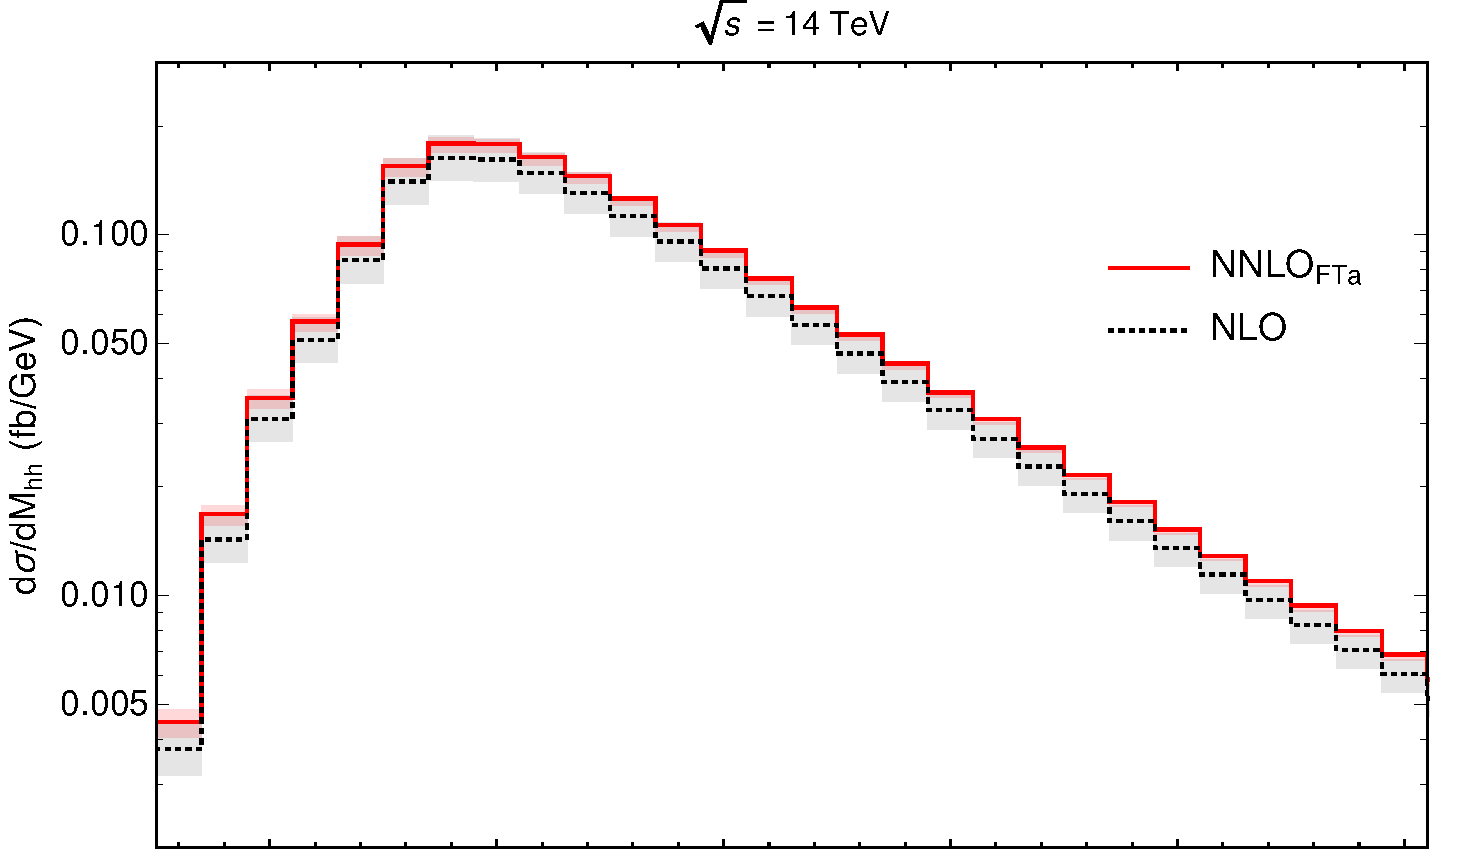
\includegraphics[width=.49\textwidth]{\main/section3/plots/14TeV_mhh}
\hfill
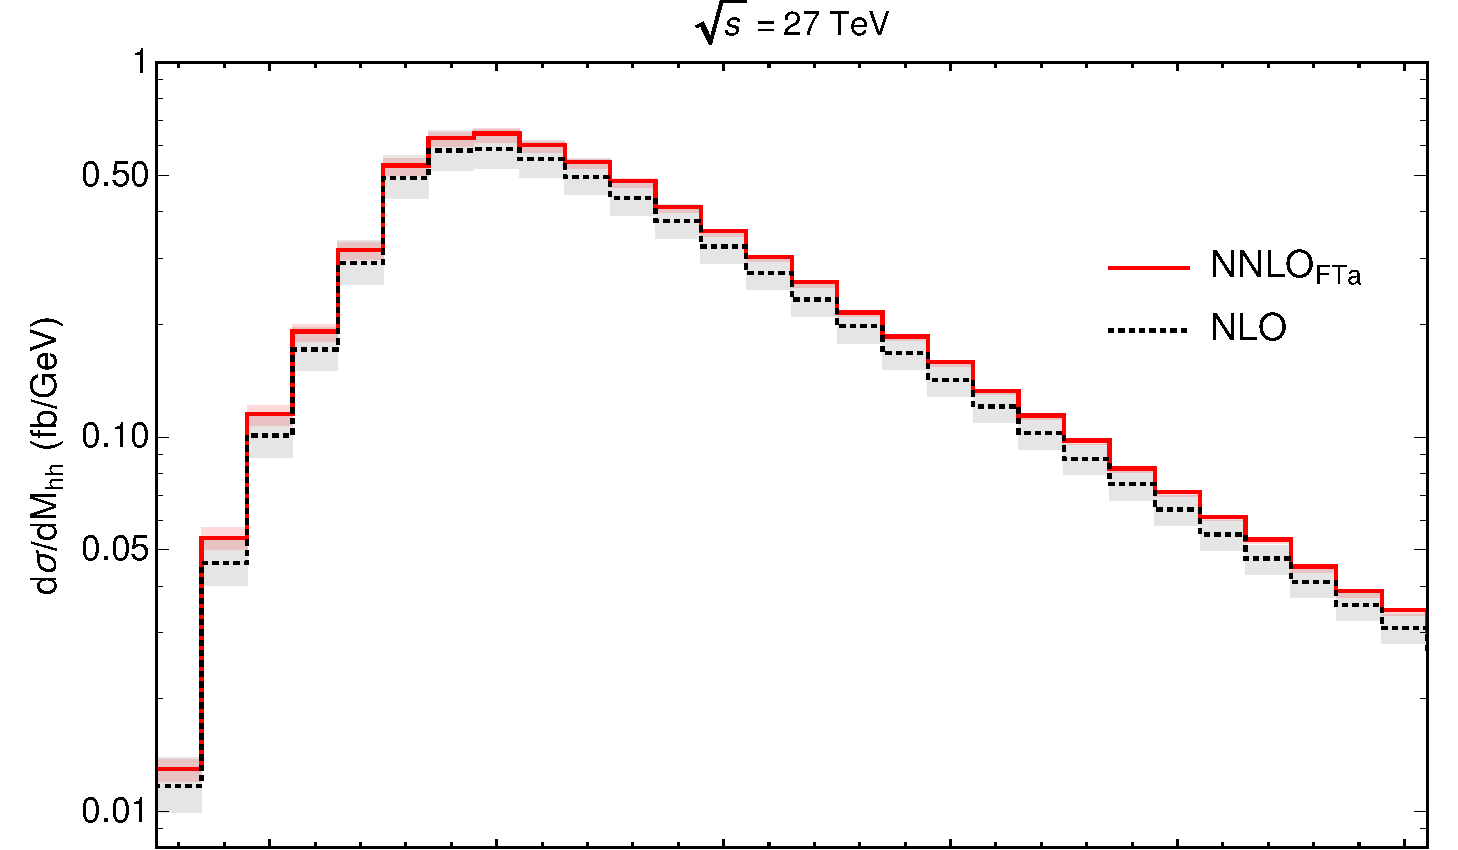
\includegraphics[width=.49\textwidth]{\main/section3/plots/27TeV_mhh}
\\
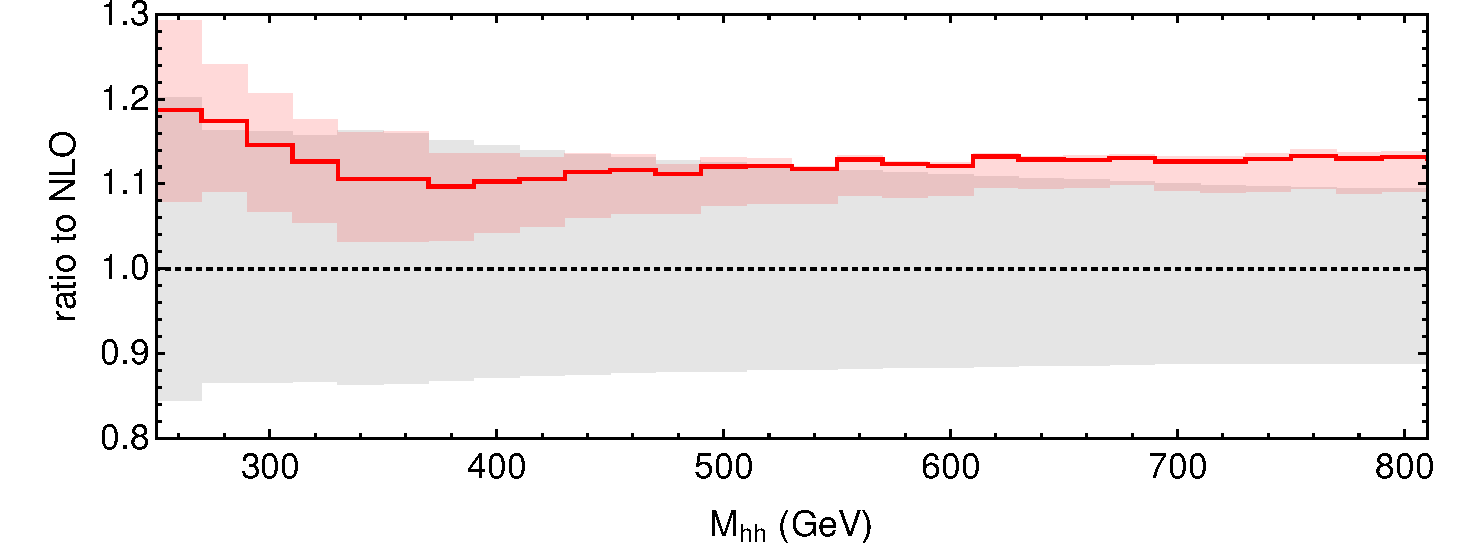
\includegraphics[width=.49\textwidth]{\main/section3/plots/14TeV_mhh_lower}
\hfill
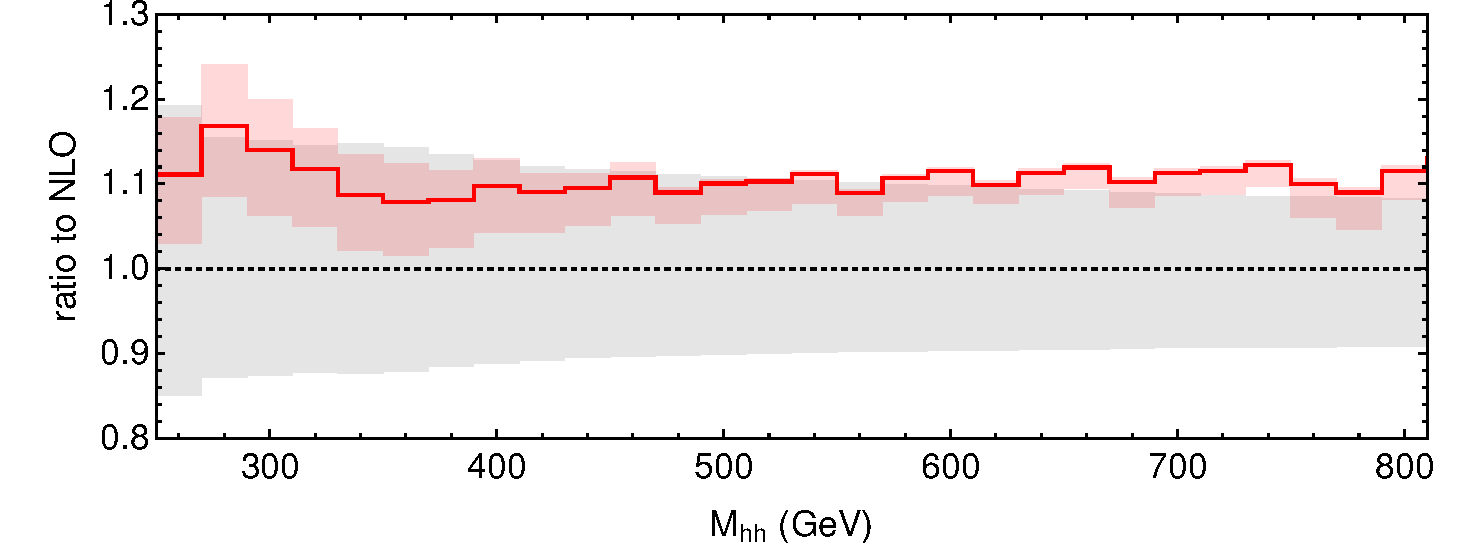
\includegraphics[width=.49\textwidth]{\main/section3/plots/27TeV_mhh_lower}
\end{center}
\vspace{-2ex}
\caption{\label{fig:mhh_NNLO}
Higgs boson pair invariant mass distribution at NNLO$_{\mathrm{FTa}}$, together with the NLO prediction, at $14\,$TeV (left) and $27\,$TeV (right). The lower panels show the ratio with respect to the NLO prediction, and the filled areas indicate the scale uncertainties.
}
\end{figure}
%%====================================


\subsubsubsection{HH production in subdominant channels}
\begin{center}
    \textit{by Eleni Vryonidou}
\end{center}

\begin{table}[h!]
\renewcommand{\arraystretch}{1.6}
\begin{center}
\resizebox{\textwidth}{!}_{-1.3\%}\pm 1.7\%$  &  $0.573^{+2.0\%}_{-1.4\%}\pm 1.9\%$  & $1.95^{+1.1\%}_{-1.5\%}\pm 2.0\%$ & $0.948^{+3.9\%}_{-13.5\%}\pm 3.2\%$& $0.0383^{+5.2\%}_{-3.3\%}\pm 4.7\%$ \\ \hline
  27 &  $0.963^{+2.1\%}_{-2.3\%}\pm 1.5\%$ & $1.48^{+2.3\%}_{-2.5\%}\pm 1.7\%$  & $8.21^{+1.1\%}_{-0.7\%}\pm 1.8\%$& $5.27^{+2.0\%}_{-3.7\%}\pm 2.5\%$&  $0.254^{+3.8\%}_{-2.8\%}\pm 3.6\%$ \\ \hline
\end{tabular}}
\end{center} 
\caption{Signal cross section (in fb) for HH production at NLO QCD.}  
\label{tab:HHxsecOthers}
\end{table}
Results  shown in Table~\ref{tab:HHxsecOthers} have been obtained within the {\sc MadGraph5\_aMC@NLO} \cite{Alwall:2014hca} framework, as in Ref. \cite{Frederix:2014hta}. The renormalisation and factorisation scale was set to $m_{HH}/2$ and varied up and down by a factor of two to obtain the scale uncertainties. The 5-flavour PDF4LHC NLO Monte Carlo PDF set was used to obtain the results (LHAPDF set number 90500, \textit {PDF4LHC15\_nlo\_mc}). The $WHH$ results are the sum of the $W^+$ and $W^-$ cross-sections. Similarly $tjHH$ involves both top and anti-top production. 

%%%%%%%%%%%%%%%%%%%%%%%%%%%%%%%%%%%%%%%%%%%%%%%%%%%%%%%%%%%%%%
%%%
%%%   subsection about variations of the trilinear coupling
%%%

\asubsubsubsection[G. Heinrich, S. Jones, M. Kerner, G. Luisoni, L. Scyboz]{Probing the Higgs boson self-coupling in di-Higgs
  production with full $m_t$-dependence at NLO QCD}
\label{subsec:varylambda}

%While the couplings of the Higgs boson to vector bosons are very well measured meanwhile, and the couplings to third generation fermions also start to be well constrained and seem to confirm the Standard Model, the Higgs boson self-coupling could still reveal clear signs of New Physics. As it is not too far-fetched to have BSM scenarios in mind where the trilinear Higgs boson coupling $\lambda$ is different from the SM value at the ${\cal O}(10\%)$ level, while the deviations in other Higgs boson couplings are at the percent level, we consider $\lambda$ variations only in this section.
In this section we consider the impact of varying the Higgs self-coupling $\lambda$ on the NLO computations of the HH production cross section.
In particular, we announce a version of the {\tt ggHH} code~\cite{Borowka:2016ypz,Heinrich:2017kxx,Borowka:2016ehy} implemented in the {\tt POWHEG-BOX-V2}~\cite{Alioli:2010xd} where variations of  $\lambda$ are accessible to the user in a parton shower Monte Carlo program at full NLO.

\asubsubsubsection{Total cross sections at different values of the trilinear coupling}

In Table \ref{tab:sigmatot} we list total cross sections at 14\,\UTeV and 27\,\UTeV for various values of the trilinear Higgs coupling $\lambda$. 
\begin{table}[htb]
\begin{center}
%\setlength{\extrarowheight}{3.0pt}
\begin{tabular}{| c | c | c |c|c|}
%\Xhline{2\arrayrulewidth}
\hline
&&&&\\
$\lambda_{\mathrm{BSM}}/\lambda_{\mathrm{SM}}$ & $\sigma_{\rm{NLO}}@14 \mathrm{\UTeV}$\,[fb] & $\sigma_{\rm{NLO}}@27 \mathrm{\UTeV}$\,[fb] &K-fac.@14TeV&K-fac.@27TeV\\
&&&&\\
\hline
1& 32.88$^{+13.5\%}_{-12.5\%}$&127.7$^{+11.5\%}_{-10.4\%}$ &1.66&1.62\\
\hline
2 & 14.91 &  59.10 & 1.58 & 1.52\\
\hline
2.4 & 13.81& 53.67 & 1.65 & 1.60\\
\hline
3& 19.82 & 69.84 & 1.97 & 1.89\\
\hline 
5 & 98.42& 330.61 & 2.21 & 2.18\\
\hline 
0 & 73.84& 275.29& 1.79 & 1.78 \\
\hline 
-1 & 137.69& 504.9 & 1.87 & 1.83\\
\hline
%\Xhline{2\arrayrulewidth}
\end{tabular}
\end{center}
\caption{Total cross sections for Higgs boson pair production at full NLO. The given uncertainties are scale uncertainties. 
\label{tab:sigmatot}}
\end{table}

The results have been obtained using the parton distribution functions PDF4LHC15\_nlo\_100\_pdfas~\cite{Butterworth:2015oua,CT14,MMHT14,Ball:2014uwa},
along with the corresponding value for $\alpha_s$ for both the NLO and
the LO calculation.
The masses have been set to $m_h=125$\,\UGeV, $m_t=173$\,\UGeV,
and the top quark width has been set to zero. 
The scale uncertainties are the result of a 7-point scale variation around the central scale $\mu_0 = m_{hh}/2$,
with $\mu_{R,F}=c_{R,F}\,\mu_0$, where 
$c_R,c_F\in \{2,1,0.5\}$, except that the extreme variations $(c_R,c_F)=(2,0.5)$ and $(c_R,c_F)=(0.5,2)$
are omitted. 

Table~\ref{tab:sigmatot} also shows that the K-factors do vary substantially as functions of the trilinear coupling.
This fact is illustrated in Fig.~\ref{fig:Kfacvariation}, where it is demonstrated that the K-factor takes values between 1.57 and 2.16.
%if the trilinear coupling is varied between $-5\leq \chhh\leq 12$.

\begin{figure}[htb]
  \centering
    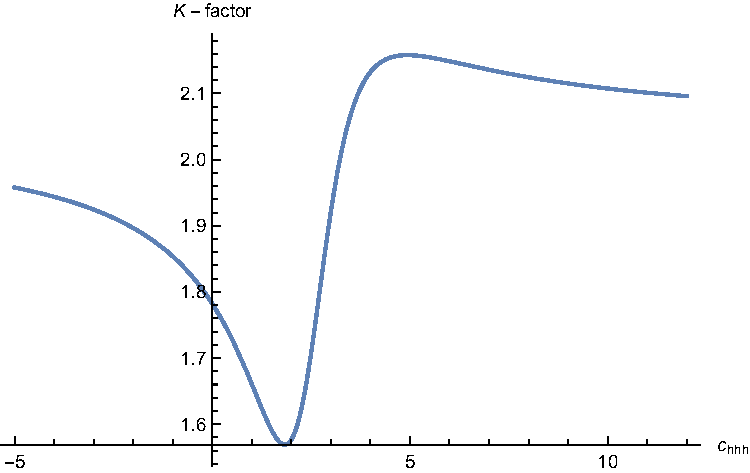
\includegraphics[width=0.4\textwidth]{\main/section3/plots/Kfac_varlambda.pdf}
%  \includegraphics[width=\textwidth]{plots/}
%    \caption{\label{fig:lambda_large_27}}
\caption{Variation of the NLO K-factor with the trilinear coupling, $\sqrt{s}=14$\,\UTeV.}
\label{fig:Kfacvariation}
\end{figure}


\asubsubsubsection{Differential cross sections  at 14 \UTeV and 27 \UTeV}

In Figs.~\ref{fig:lambda_small} and ~\ref{fig:lambda_large} we show the $\mhh$ distribution for various values of $\lambda=\lambda_{\mathrm{BSM}}/\lambda_{\mathrm{SM}}$ at 14 \UTeV.
Figs.~\ref{fig:lambda_small_27} and ~\ref{fig:lambda_large_27} 
 show results for the $\mhh$ distribution at 27 \UTeV. The scale variation band for $\lambda=1$ is also included.
 Note that $\lambda=2.4$ is the value where the cross section as a function of $\lambda$ goes through a minimum, due to maximal destructive interference between diagrams containing the trilinear coupling and diagrams which do not contain Higgs boson self-couplings.
 
\begin{figure}[htb]
  \centering
  \subfloat[]{\label{fig:lambda_small_14}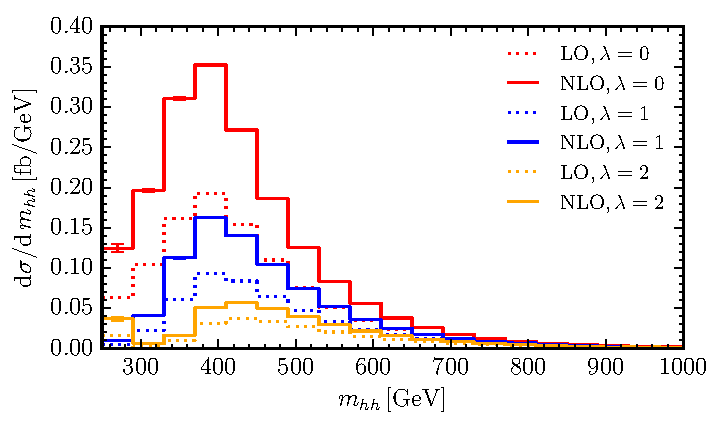
\includegraphics[width=0.6\textwidth]{\main/section3/plots/mhh_Kfac_14TeV_varylambda_small.pdf}}
  %\hfill
  %\subfloat[]{\label{fig:lambda_small_27}}
  %  \includegraphics[width=\textwidth]{plots/}
 \caption{Higgs boson pair invariant mass distributions for various values of $\lambda$ (relative to $\lambda_{\mathrm{SM}}$)  at 14\,\UTeV.}
\label{fig:lambda_small}
\end{figure}
%
\begin{figure}[htb]
  \centering
    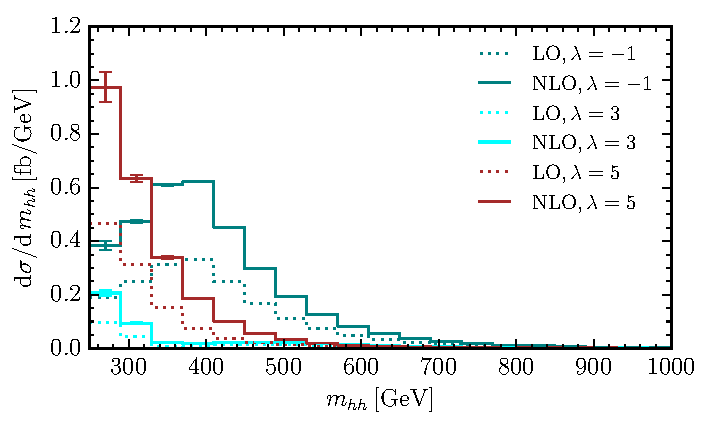
\includegraphics[width=0.6\textwidth]{\main/section3/plots/mhh_Kfac_14TeV_varylambda_large.pdf}
%  \includegraphics[width=\textwidth]{plots/}
%    \caption{\label{fig:lambda_large_27}}
\caption{Higgs boson pair invariant mass distributions for $\lambda=\lambda_{\mathrm{BSM}}/\lambda_{\mathrm{SM}}=-1,3,5$  at 14\,\UTeV.}
\label{fig:lambda_large}
\end{figure}

\begin{figure}[htb]
  \centering
    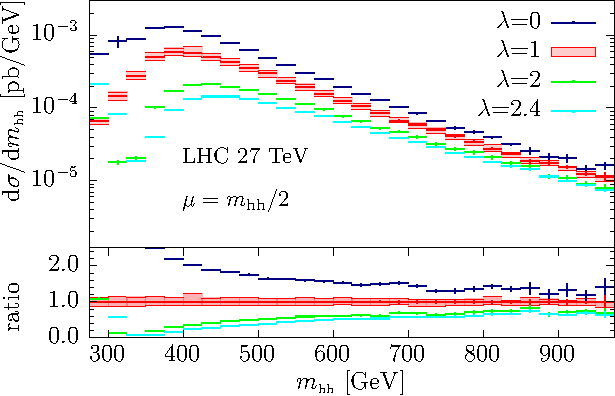
\includegraphics[width=0.6\textwidth]{\main/section3/plots/NLO_mHH_small_lambda_27TeV.pdf}
%  \includegraphics[width=\textwidth]{plots/}
%    \caption{\label{fig:lambda_large_27}}
\caption{Higgs boson pair invariant mass distributions for $\lambda=\lambda_{\mathrm{BSM}}/\lambda_{\mathrm{SM}}=0,1,2,2.4$  at 27\,\UTeV. The scale uncertainties for the SM value of $\chhh$ are shown as a red band.}
\label{fig:lambda_small_27}
\end{figure}

\begin{figure}[htb]
  \centering
    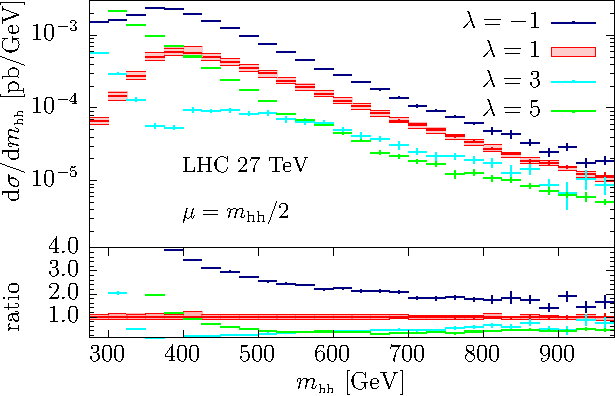
\includegraphics[width=0.6\textwidth]{\main/section3/plots/NLO_mHH_large_lambda_27TeV.pdf}
%  \includegraphics[width=\textwidth]{plots/}
%    \caption{\label{fig:lambda_large_27}}
\caption{Higgs boson pair invariant mass distributions for $\lambda=\lambda_{\mathrm{BSM}}/\lambda_{\mathrm{SM}}=-1,1,3,5$  at 27\,\UTeV. The scale uncertainties for the SM value of $\lambda$ are shown as a red band.}
\label{fig:lambda_large_27}
\end{figure}

\begin{figure}[ht]
\begin{center}
  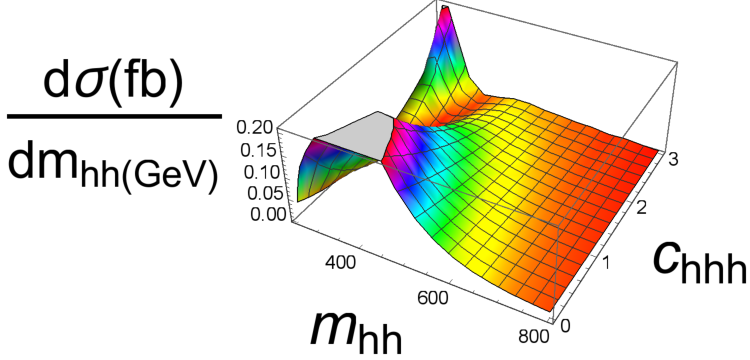
\includegraphics[width=0.45\textwidth]{\main/section3/plots/3D_mhh_chhh.pdf}    
\end{center}
\caption{3-dimensional visualisation of the $\mhh$ distribution at
  14\,\UTeV, as a function  $\lambda$.}
\label{fig:chhh_3D}
\end{figure}
Fig.~\ref{fig:chhh_3D} shows the Higgs boson pair invariant mass
distributions at NLO as a function of $\lambda=\chhh$  as a 3-dimensional heat map.
The dip in the distribution around $\chhh=2.4$ is clearly visible.
 
%\bibliography{bib/refs_HH_lambda}





%%%%%%%%%%%%%%%%%%%%%%%%%%%%%%%%%%%%%%%%%%%%%%%%%%%%%%%%%%%%%% 

%%%
%%%   nonlinear EFT subsection
%%%

\subsubsection{Di-Higgs production in the non-linear EFT with full $m_t$-dependence at NLO QCD}

\begin{center}
\textit{by Gerhard Buchalla, Alejandro Celis, Matteo Capozi, Gudrun Heinrich, Ludovic Scyboz}
\end{center}


\subsubsubsection{The Higgs sector in the non-linear EFT framework}
\label{sec:EWChL.double.h}

Below we will describe  the potential impact of physics
beyond the Standard Model through a non-linear Effective Field Theory,
also called the electroweak chiral Lagrangian
including a light Higgs 
boson~\cite{Buchalla:2013rka,Buchalla:2013eza,Buchalla:2017jlu}.
This framework provides us with a consistent EFT
for New Physics in the Higgs sector, where the Higgs field is an electroweak singlet $h$,
independent of the Goldstone matrix $U = \exp(2i\varphi^a T^a/v)$.
The latter transforms as $U\to g_L U g^\dagger_Y$ under the SM gauge group.
The symmetry is non-linearly realised on the Goldstone fields
$\varphi^a$, therefore the name non-linear EFT.
More details about this framework already have been given in
Section~\ref{sec:2:kappavsEFT}.
Therefore we restrict ourselves to stating the part of the Lagrangian
relevant for our study of anomalous Higgs couplings:
\begin{align}
{\cal L}\supset 
-m_t\left(c_t\frac{h}{v}+c_{tt}\frac{h^2}{v^2}\right)\,\bar{t}\,t -
c_{hhh} \frac{m_h^2}{2v} h^3+\frac{\alpha_s}{8\pi} \left( c_{ggh} \frac{h}{v}+
c_{gghh}\frac{h^2}{v^2}  \right)\, G^a_{\mu \nu} G^{a,\mu \nu}\;.
\label{eq:ewchl}
\end{align}
To lowest order in the SM $c_t=c_{hhh}=1$ and $c_{tt}=c_{ggh}=c_{gghh}=0$.
In general, all couplings may have arbitrary values of ${\cal O}(1)$.
Note that we have extracted a loop factor from the definition of the
Higgs-gluon couplings.  


The leading-order diagrams are shown in Fig.~\ref{fig:hprocess}.
\begin{figure}[htb]
\begin{center}
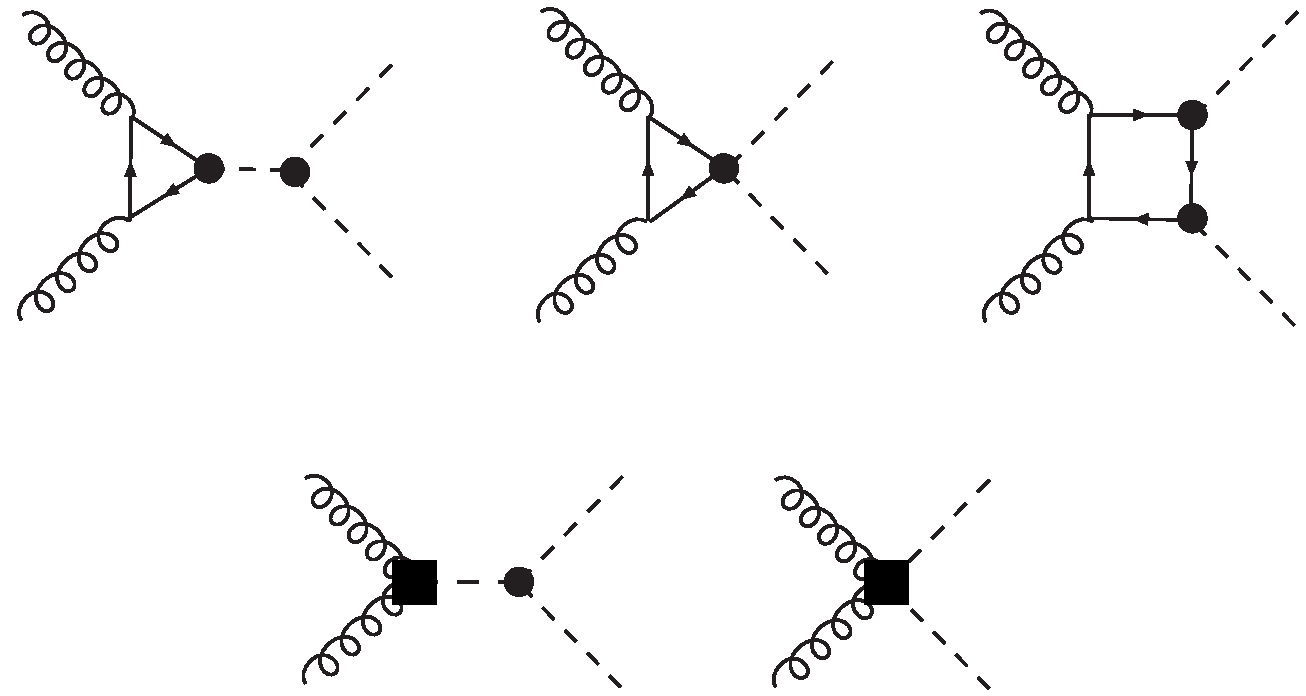
\includegraphics[width=7.5cm]{\main/section3/plots/hprocess.pdf}
\end{center}
\caption{Higgs-pair production in gluon fusion at leading order
in the non-linear EFT Lagrangian.}
\label{fig:hprocess}
\end{figure}
Examples for virtual diagrams at NLO are shown in
Fig.~\ref{fig:virt_examples}.
For further details we refer to Ref.~\cite{Buchalla:2018yce}.
\begin{figure}[htb]
\begin{center}
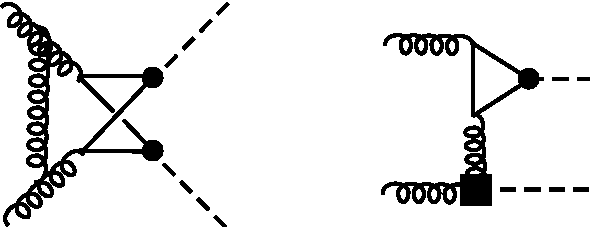
\includegraphics[width=6cm]{\main/section3/plots/hpnloyr1.pdf}
\end{center}
\caption{Examples of virtual diagrams contributing at NLO QCD.}
\label{fig:virt_examples}
\end{figure}


\subsubsubsection{Total cross sections for 14 and 27 TeV at some benchmark points}

In the following we will show results for some benchmark points, specified in Table~\ref{tab:benchmarks}, 
some of them having been first defined in Refs.~\cite{Carvalho:2015ttv}.
The results at 14\,TeV and 27\,TeV are given in Table~\ref{sigmatot}.
Note that our conventions for $\cg$ and $\cgg$ differ from the ones in
Ref.~\cite{Carvalho:2015ttv,Carvalho:2016rys}, the relations are $c_{ggh}= \frac{2}{3}c_g $
and $c_{gghh}=-\frac{1}{3}c_{2g}$, where $c_g,c_{2g}$ are the
couplings defined in Refs.~\cite{Carvalho:2015ttv,Carvalho:2016rys}.
We also take into account recent constraints on $\cg$ from
Refs.~\cite{CMS-PAS-HIG-17-031,deBlas:2018tjm}
and the  limits on the Higgs boson pair production cross section
from Refs~\cite{CMS-PAS-HIG-17-030,ATLAS-CONF-2018-043}.
This is why we do not show results for the original benchmark point 5
anymore, as its value for $\cg$ is outside the 2-sigma band of a
combined fit of $\cg,\ct$ from single Higgs production
data~\cite{CMS-PAS-HIG-17-031,deBlas:2018tjm}.
Benchmark point 6 is interesting because its value for $\chhh$ is near
the point where maximal destructive interference takes place between
triangle-type and box-type contributions if the other couplings are SM-like, leading to a total cross
section which is below the SM value.

\begin{table}[htb]
\begin{center}
%\setlength{\extrarowheight}{3.0pt}
%\scalebox{1.}{%
\begin{tabular}{| c | c  c  c  c  c |}
%\Xhline{2\arrayrulewidth}
\hline
Benchmark & $c_{hhh}$ & $c_t$ & $c_{tt}$ & $c_{ggh}$ & $c_{gghh}$ \\
\hline
5a & 1 & 1 & 0 &   $2/15$ & $4/15$\\
\hline
6 & 2.4 & 1 & 0 & $2/15$ & $1/15$  \\
\hline
7 & 5 & 1 & 0 & $2/15$ & $1/15$  \\
\hline
8a & 1 & 1 & 1/2 & $4/15$ & 0\\
\hline
SM & 1 & 1 & 0 & 0 & 0 \\
\hline
%\Xhline{2\arrayrulewidth}
\end{tabular}
\end{center}
\caption{Benchmark points used for the distributions shown below.\label{tab:benchmarks}}
\end{table}
%
\begin{table}[htb]
\begin{center}
\begin{tabular}{|c|c|c|c|c|c|}
\hline
&&&&&\\
Benchmark & $\sigma_{NLO}$ [fb] & K-factor & scale uncert.  &
stat. uncert.   &$\frac{\sigma_{NLO}}{\sigma_{NLO,SM}}$ \\ 
&&&[\%] &[\%] &\\
\hline
$    B_{5a}$ [14 TeV] & 38.64 & 1.78& ${+3.7, \; -12}$ &0.24  &1.17  \\ 
$    B_{5a}$ [27 TeV] & 198.64 & 1.75 & ${+2.1, \; -10}$ & 0.43 & 1.56  \\ 
\hline
$    B_{6}$ [14 TeV] &  24.69 & 1.89 & ${+2, \; -11}$ & 2.1 & 0.75 \\ 
$    B_{6}$ [27 TeV] &  97.25 &  1.58& ${+0.53, \; -5.6}$ &1.63  & 0.76  \\ 
\hline
$   B_7$ [14 TeV] & 169.41 & 2.07& ${+9, \; -12}$ & 2.2 & 5.14 \\
$   B_7$ [27 TeV] & 598.20 & 2.11 & ${+8, \; -10}$ & 2.0 &  4.68\\
\hline 
$   B_{8a}$ [14 TeV] & 41.70 & 2.34& ${+6, \; -9}$ & 0.63 & 1.27 \\
$   B_{8a}$ [27 TeV] & 179.52 & 2.33 & ${+4, \; -7}$ & 0.49 & 1.40 \\
\hline 
$   SM $ [14 TeV] & 32.95 & 1.66 & ${+14, \; -13}$ & 0.1 & 1\\
$   SM $ [27 TeV] & 127.7&  1.62 & ${+12, \; -10}$ & 0.1 & 1\\
\hline
\end{tabular}
\end{center}
\caption{Total cross sections at 14 and 27 TeV at NLO (2nd column),
K-factor $\sigma_{NLO}/\sigma_{LO}$ (3rd column),
scale uncertainty (4th column), statistical uncertainty (5th column)
and the ratio to the SM total cross section at NLO (6th column).\label{sigmatot}}
\end{table}
%
% \begin{table}[htb]
% \begin{center}
% \begin{tabular}{|c|c|c|c|c|}
% \hline
%  & $B_5$ & $B_7$ & $B_{8a}$& SM\\
% \hline
% $\frac{\sigma_{NLO}[27\,\mathrm{TeV}]}{\sigma_{NLO}[14\,\mathrm{TeV}]}$& 5.10& 3.53& 4.31& 3.88\\
% \hline
% \end{tabular}
% \end{center}
% \caption{Ratios of total cross sections at 14\,TeV and 27\,TeV at NLO.\label{energy_ratios}}
% \end{table}
Table~\ref{sigmatot} shows that the total cross sections increase by a factor of 3.5-5 when increasing the centre-of-mass energy from 14\,TeV to 27\,TeV. The increase for $B_{5a}$ is largest because of the large value of $\cgg$, which yields a contribution growing linearly with energy.

%\clearpage


\subsubsubsection{HH  invariant mass distributions at 14 and 27 TeV at some benchmark points}

In Figs.~\ref{fig:benchmark7} and \ref{fig:benchmark8a} we show Higgs boson pair invariant mass distributions for the benchmark points 7 and 8a. 
For both of them the shape of the distribution is very different from the SM one, and the K-factor is non-homogeneous over the whole $\mhh$-range. Benchmark point 7 is characterised by a large enhancement of the low $\mhh$ region, induced by the large value of $\chhh$. The lower ratio plot shows the ratio of the two approximations ``Born-improved HEFT" and ``FT$_{\rm{approx}}$" to the full NLO, where the former denotes the $m_t\to\infty$ limit rescaled by the $m_t$-dependent LO, while FT$_{\rm{approx}}$ includes the Born-improved $m_t\to\infty$ limit for the virtual part and the full $m_t$-dependence for the real radiation part. One can see from Fig.~\ref{fig:benchmark7} that these approximations are off by about 20\% even below the $2m_t$ threshold. Therefore one cannot claim that the $m_t\to \infty$ limit works well in the region below $\sim 400$\,GeV. As the triangle-type contributions are dominating for $\chhh=5$, their full $m_t$-dependence plays a significant role. 

Benchmark point 8a shows a characteristic dip near $\mhh=2\,m_t$ and an enhancement in the tail compared to the SM. 
As the total cross section for $B_{8a}$ is very similar to the SM one, both at 14\,TeV and at 27\,TeV, this is an example where the discriminating power of differential information is very important.

\begin{figure}[htb]
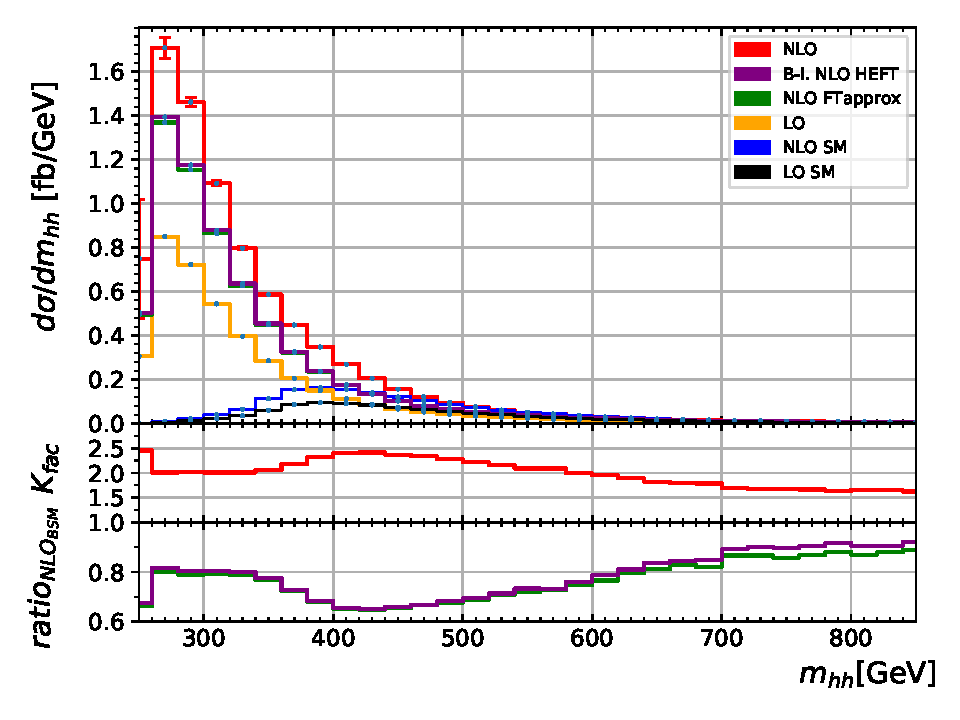
\includegraphics[width=0.48\textwidth]{\main/section3/plots/Ben_7_mhh.pdf}
~
 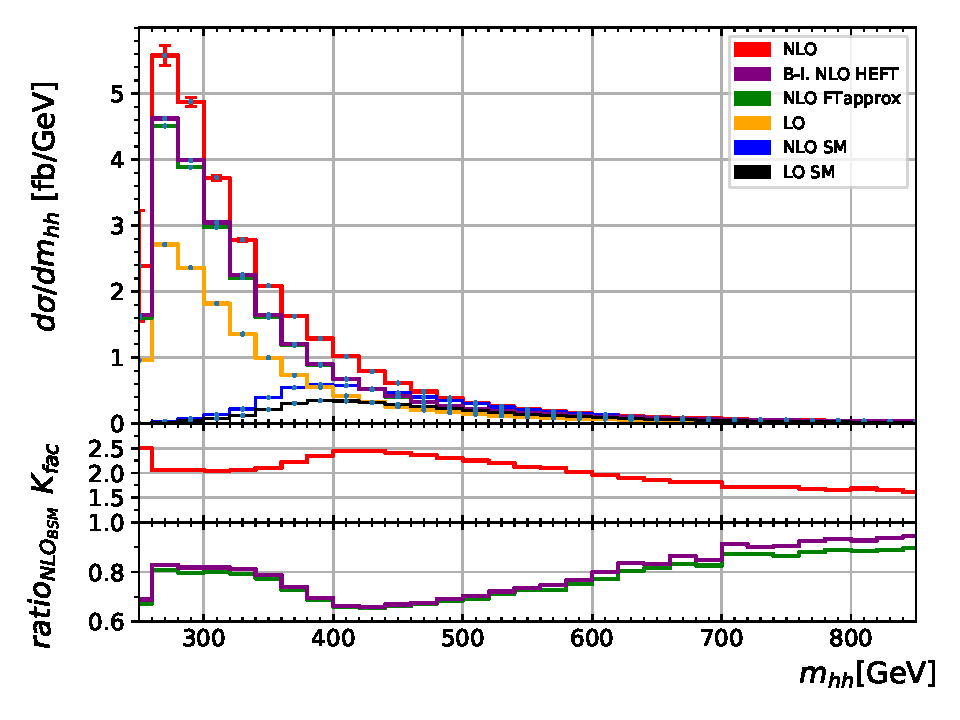
\includegraphics[width=0.48\textwidth]{\main/section3/plots/Ben_7_mhh_27TeV.pdf}
\caption{Higgs boson pair invariant mass distributions  for benchmark point 7, $\chhh=5,\ct= 1, \ctt=0, \cg=2/15,\cgg=1/15$, at 14\,TeV (left) and 27\,TeV (right).}
\label{fig:benchmark7}
\end{figure}
%
\begin{figure}[htb]
  \centering
  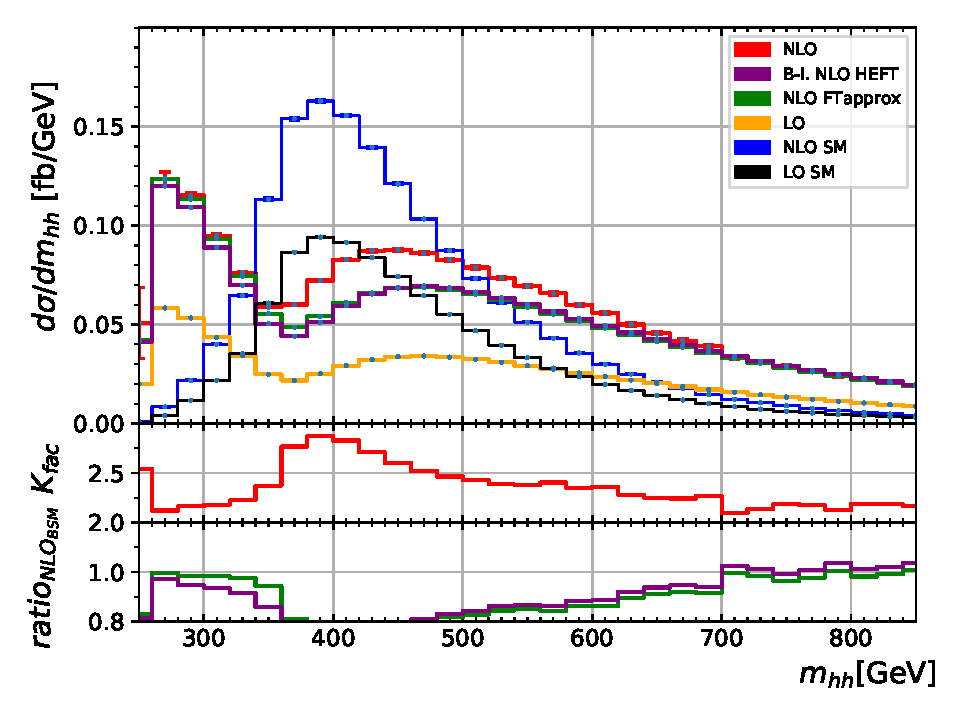
\includegraphics[width=0.48\textwidth]{\main/section3/plots/Ben_8a_mhh.pdf} 
~
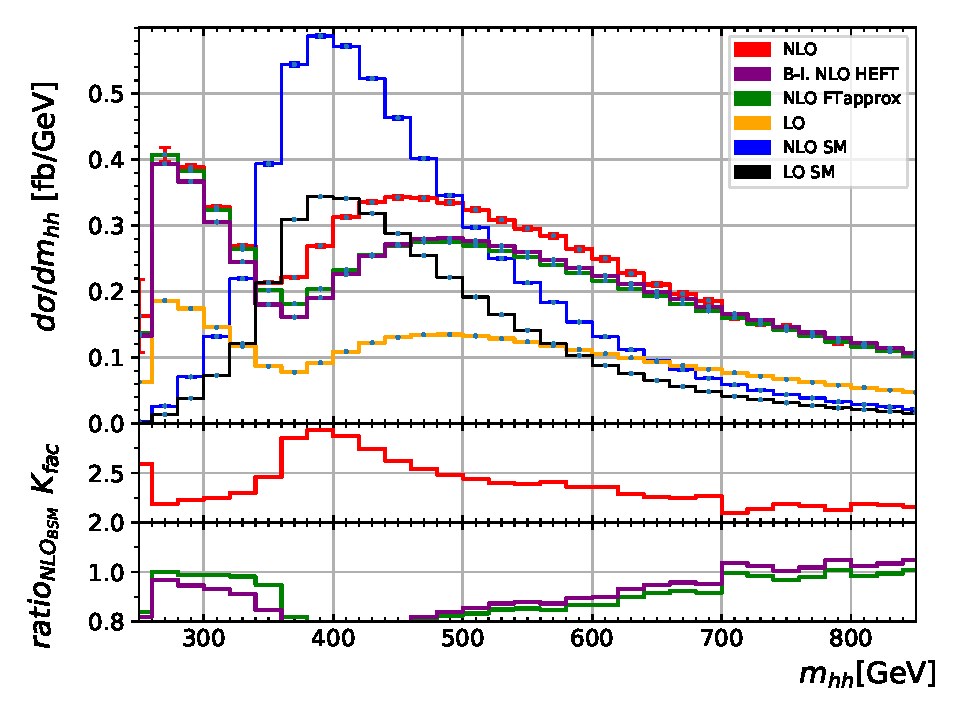
\includegraphics[width=0.48\textwidth]{\main/section3/plots/Ben_8a_mhh_27TeV.pdf}
\caption{Higgs boson pair invariant mass distributions  for benchmark point 8a, $\chhh=1,\ct= 1, \ctt=0.5, \cg=4/15,\cgg=0$, at 14\,TeV (left) and 27\,TeV (right).}
\label{fig:benchmark8a}
\end{figure}
%



\subsubsubsection{Characterising the BSM parameter space}

The total cross section can be written in terms of the 15 coefficients 
$A_1, \ldots, A_{15}$, at LO~\cite{Carvalho:2015ttv,Azatov:2015oxa} and in terms of 23 coefficients at NLO~\cite{Buchalla:2018yce}.
%
\begin{align}
\label{eq:Acoeffs_all}
&\sigma^{\rm{NLO}}/\sigma^{\rm{NLO}}_{SM}  =\nn\\
& \quad  A_1\, c_t^4 + A_2 \, c_{tt}^2  + A_3\,  c_t^2 \chhh^2  + 
A_4 \, \cg^2 \chhh^2  + A_5\,  \cgg^2  + 
A_6\, c_{tt} c_t^2 + A_7\,  c_t^3 \chhh \nn\\
& + A_8\,  c_{tt} c_t\, \chhh  + A_9\, c_{tt} \cg \chhh + A_{10}\, c_{tt} \cgg + 
A_{11}\,  c_t^2 \cg \chhh + A_{12}\, c_t^2 \cgg \nn\\
& + A_{13}\, c_t \chhh^2 \cg  + A_{14}\, c_t \chhh \cgg +
A_{15}\, \cg \chhh \cgg \nn\\ 
& + A_{16}\, c^3_t \cg + A_{17}\,  c_t c_{tt} \cg 
+ A_{18}\, c_t \cg^2 \chhh + A_{19}\, c_t \cg \cgg 
\nn\\
&+ A_{20}\,  c_t^2 \cg^2 + A_{21}\, c_{tt} \cg^2 
+ A_{22}\, \cg^3 \chhh + A_{23}\, \cg^2 \cgg\,.
\end{align}
Based on our results for $A_1,\ldots, A_{23}$, we produce heat maps for the ratio $\sigma/\sigma_{SM}$, 
varying two of the five parameters, while for the fixed parameters the SM values are used, along with
$\sigma_{SM}^{\rm{LO}}[14\,\mathrm{TeV}]=19.85$\,fb,
$\sigma_{SM}^{\rm{NLO}}[14\,\mathrm{TeV}]=32.95$\,fb.
The couplings are varied in a range which seems reasonable when taking into account the current constraints on the 
Higgs coupling measurements
%~\cite{Khachatryan:2016vau}, 
as well as recent limits on the di-Higgs production cross
section~\cite{CMS-PAS-HIG-17-030,ATLAS-CONF-2018-043}.

%
\begin{figure}[ht]
\begin{center}
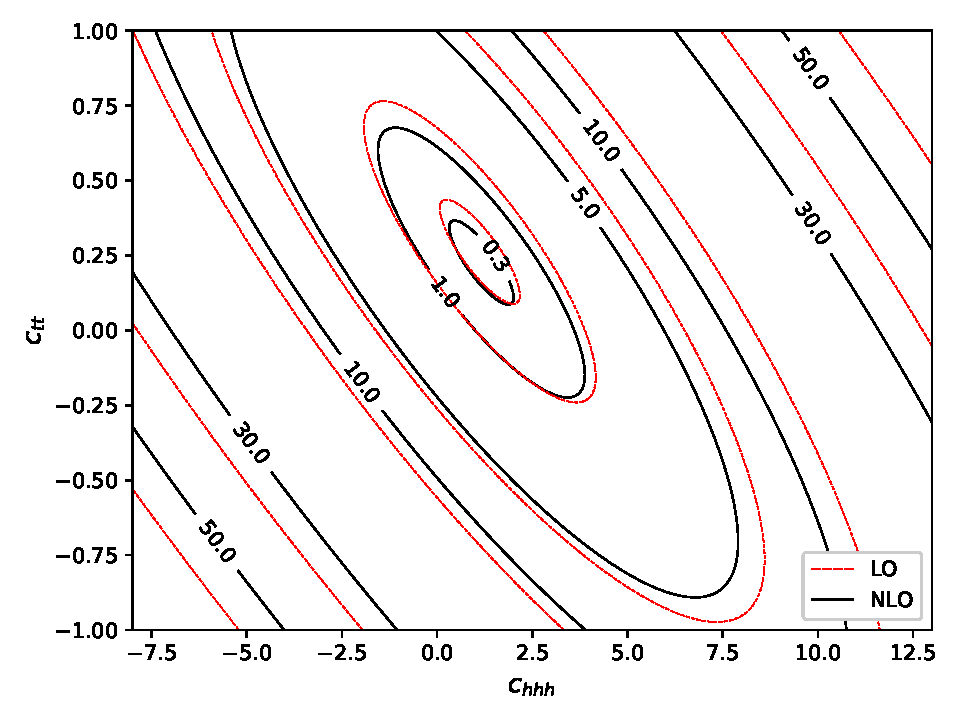
\includegraphics[width=0.45\textwidth]{\main/section3/plots/plot_chhh_ctt.pdf}    
~
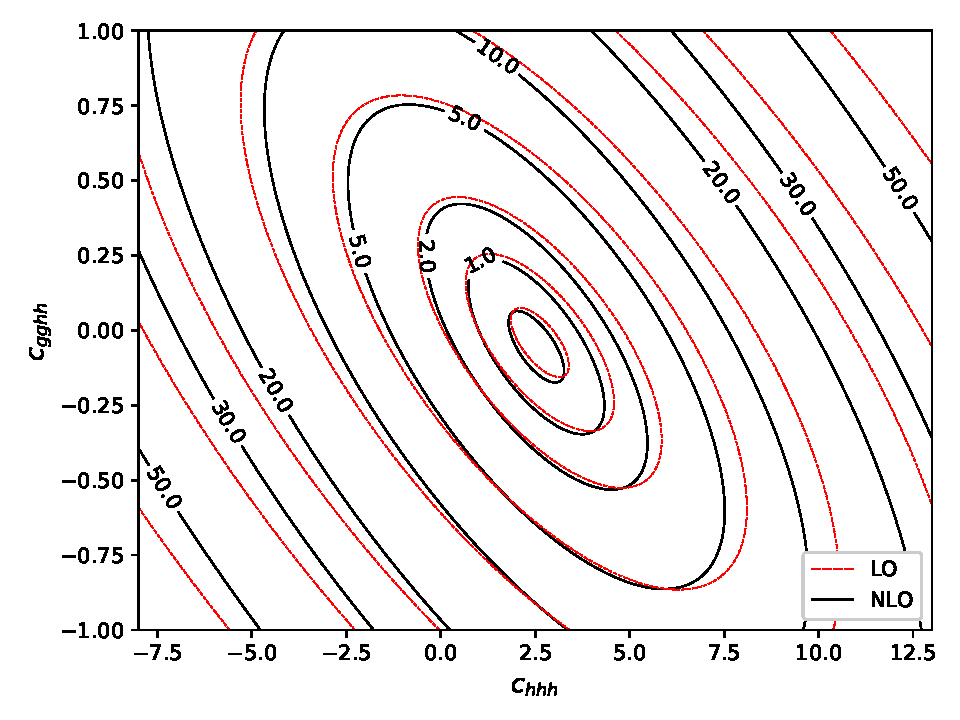
\includegraphics[width=0.45\textwidth]{\main/section3/plots/plot_chhh_cgghh.pdf}
\end{center}
\caption{Iso-contours of $\sigma/\sigma_{SM}$: (a) $\chhh$ versus $\ctt$ and (b) $\chhh$ versus $\cgg$  at $\sqrt{s}=14$\,TeV.}
\label{fig:chhh_ctt_cgg}
\end{figure}

Fig.~\ref{fig:chhh_ctt_cgg} shows variations of the triple Higgs coupling $\chhh$ in combination with $\ctt$ and $\cgg$ at $\sqrt{s}=14$\,TeV.
%The range for $\chhh$ is chosen according to the most recent experimental constraints~\ref{Aaboud:2018ft}.
We observe that the deviations from the SM cross section can be substantial.
%
\begin{figure}[ht]
\begin{center}
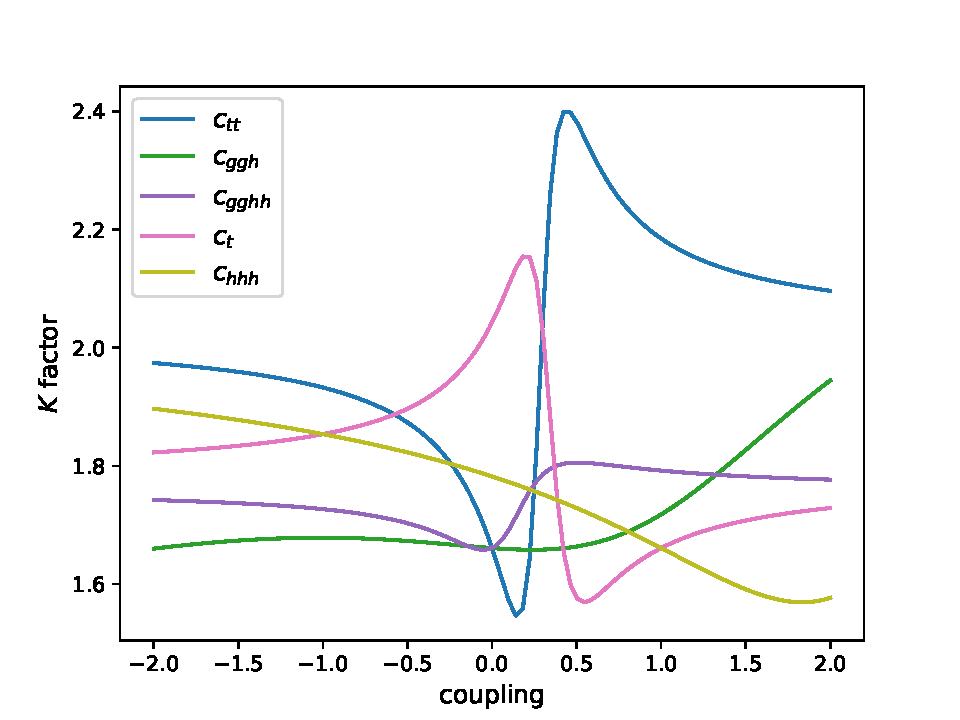
\includegraphics[width=9cm]{\main/section3/plots/Kplot.pdf}
\end{center}
\caption{K-factors for the total cross section at $\sqrt{s}=14$\,TeV as a function of the
  different couplings.}
\label{fig:project_ctt}
\end{figure}
%
In Fig.~\ref{fig:project_ctt} we show the K-factors as a function of
the coupling parameters, with the others fixed to their SM values. 
It shows that the K-factors exhibit a much stronger dependence on the
coupling parameters once the full top quark mass dependence is taken into account when compared to 
the results in the $m_t\to\infty$ limit~\cite{Grober:2015cwa,deFlorian:2017qfk}.
%

Fig.~\ref{fig:ctt_3D} shows the Higgs boson pair invariant mass
distributions as a function of (a) $\ctt$ and (b) $\cgg$ as 3-dimensional heat maps.
In case (a) the other couplings are fixed to their SM values.
We can see that large values of $|\ctt|$ lead to a substantial increase of the cross section, in particular at low $\mhh$ values.
%  
\begin{figure}[ht]
\begin{center}
  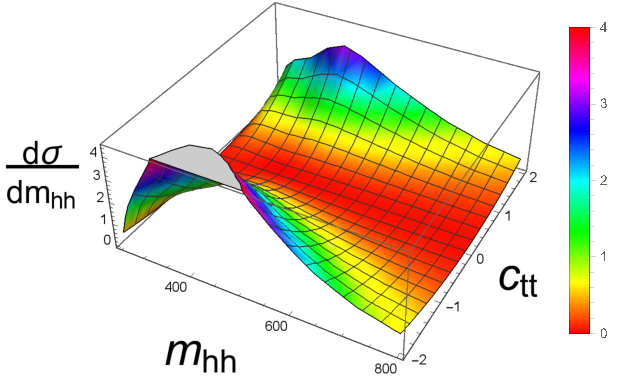
\includegraphics[width=0.45\textwidth]{\main/section3/plots/3D_mhh_ctt.pdf}    
~
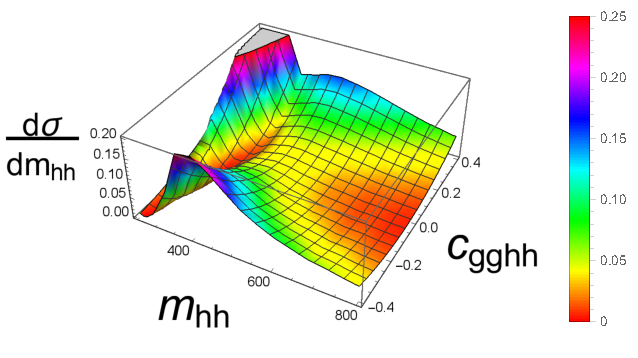
\includegraphics[width=0.5\textwidth]{\main/section3/plots/3D_mhh_cgghh_lam24.pdf}
\end{center}
\caption{3-dimensional visualisation of the $\mhh$ distribution (in units of fb/GeV) at 14\,TeV as a function of (a) $\ctt$  and (b) $\cgg$.  In case (a) all
other couplings are fixed to their SM values, in case (b) $\chhh= 2.4$.}
\label{fig:ctt_3D}
\end{figure}
In case (b) the other couplings are fixed to their SM values except for $\chhh$, which is fixed to $\chhh=2.4$
in order to demonstrate the following point: varying only $\chhh$, the $\mhh$ distribution shows a dip in the differential cross section just below $\mhh\sim 2m_t$ for $\chhh\sim 2.4$, while the low $\mhh$ region gets enhanced for larger values of $\chhh$, see Section~\ref{subsec:varylambda}.
 However, this pattern can get destroyed by non-zero
 Higgs-gluon contact interactions. While $\cg$ is increasingly well constrained meanwhile,
 $\cgg$ still could be relatively large. We can see from Fig.~\ref{fig:ctt_3D}(b) that the dip is not present for very low (negative) $\cgg$ values and also gets very shallow for values of $\cgg\sim 0.4$.
 Therefore it would be premature to conclude that a dip in the $\mhh$ distribution points to a value of $\chhh$ close to 2.4.

We also point out that the LO and NLO $A_i$ coefficients for both the total cross
section and the $\mhh$ distributions at both 14\,TeV and 27\,TeV are
available as ancillary files coming with Ref.~\cite{Buchalla:2018yce}. These data files allow to reconstruct the full NLO result for any point in the 5-dimensional parameter space.


%\clearpage

%\subsubsubsection{Conclusions}


%%%%%%%%%%%%%%%%%%% 
%%%%%%%%%%%%%%%%%%%%%%%%%%%%%%%%%%%%%%%%%%%
\subsection{Double Higgs measurements and trilinear coupling: experimental prospects}
\label{sec:HH_meas_exp}

The current Run 2 measurements of the Higgs-boson-pair production are performed with approximately 36~$fb^{-1}$ of collision data at a centre-of-mass energy of 13~TeV, combining different decay channels~\cite{ATLAS-CONF-2018-043, Sirunyan:2018two}. 
The ATLAS collaboration reports the combined observed (expected) limit on the non-resonant Higgs-boson-pair production cross-section of 6.7 (10.4) times the SM expectation. The ratio of the Higgs boson self-coupling to its SM expectation is observed (expected) to be constrained at 95\% CL to $-5.0<\kappa_{\lambda}<12.1$ ($-5.8<\kappa_{\lambda}<12.0$). 
The reported combined observed (expected) limit on the non-resonant Higgs-boson-pair production cross-section by the CMS collaboration is 22.2 (12.8) times the predicted Standard Model cross-section. The ratio of the Higgs boson self-coupling to its SM expectation is observed (expected) to be constrained at 95\% CL to $-11.8<\kappa_{\lambda}<18.8$ ($-7.1<\kappa_{\lambda}<13.6$). 

Either those measurements were extrapolated to the centre-of-mass energy of 14~TeV and integrated luminosity of 3000~\ifb, either dedicated samples were used. Parameterised functions were used to estimate the response of the upgraded ATLAS and CMS detectors at the HL-LHC. The average number of additional proton-proton interactions (pile-up) per bunch crossing is assumed to be $<\mu>$ = 200.

Only the production of HH pairs through gluon-gluon fusion is considered, with an expected cross-section of 36.69$^{+2.1\%}_{-4.9\%}$ fb at 14 TeV~\cite{Grazzini:2018bsd}. The state of the art NNLO/NNLL calculation with finite top mass effects included at NLO in QCD is used, for a Higgs boson mass of 125 \UGeV. Scale uncertainties are reported as superscript/subscript. The estimated top quark mass uncertainty of the NNLOFTapprox predictions is also presented, together with PDF and $\alpha_{S}$ uncertainties. PDF uncertainties are estimated within the Born-improved approximation. The calculation is performed in the on-shell top quark mass scheme, and studies of the uncertainty related to the scheme choice are in progress. 

\subsubsection{Measurements with the ATLAS experiment}
\label{sec:HH_ATLAS}

\subfile{\main/section3/HHmeasurement_ATLAS}

\subsubsection{Measurements with the CMS experiment}
\label{sec:HH_CMS}

\begin{center}
\textit{by A. Benaglia, M. Bengala, O. Bondu, L. Borgonovi, S. Braibant, L. Cadamuro, A. Carvalho, C. Delaere, M. Delcourt, N. de Filippis, E. Fontanesi, M. Gallinaro, M. Gouzevitch, J. R. Komaragiri, D. Majumder, K. Mazumdar, F. Monti, G. Ortona, L. Panwar, N. Sahoo, R. Santo, G. Strong, M. Vidal, S. Wertz}
\end{center}

The work described in this section studies the prospects for \HH production at the HL-LHC with the CMS experiment.
The five decay channels \bbbb, \bbtt, \bbWW ($\PW\PW\to\ell\nu\ell'\nu'$ with $\ell,\ell' = \Pe,\Pgm$), \bbgg, and \bbZZ ($\PZ\PZ\to\ell\ell\ell'\ell'$ with $\ell,\ell' = \Pe,\Pgm$) are explored.
The corresponding branching fractions and the total number of \HH events expected to be produced at the HL-LHC assuming $\sqrt{s} = 14\TeV$ and an integrated luminosity of $3000\fbi$ are reported in Table~\ref{sec3:CMSHH:tab:br_nevent}.

A short description of the analysis strategy and of the results is given here, and further details can be found in Ref.~\cite{CMS-PAS-FTR-18-019}.

\begin{table}[h]
  \begin{center}
    \caption{Branching fraction of the five decay channels considered in the CMS \HH prospects, and corresponding number of events produced at the end of HL-LHC operations assuming $\sqrt{s} = 14\TeV$ and an integrated luminosity of $3000\fbi$. The symbol $\ell$ denotes either a muon or an electron. In the \bbWW decay channel, $\ell$ from the intermediate production of a $\tau$ lepton are also considered in the branching fraction.}
    \label{sec3:CMSHH:tab:br_nevent}
    \begin{tabular}{l  ccccc}
        \hline
        Channel            & $\bbbb$ & $\bbtt$ & $\bbWW(\ell\nu\ell\nu)$ & $\bbgg$ & $\bbZZ(\ell\ell\ell\ell)$ \\
        $\mathcal{B}$ [\%] & 33.9    & 7.3     & 1.7                    & 0.26    & 0.015\\
        Number of events   & 37000   & 8000    & 1830                   & 290     & 17\\
        \hline      
    \end{tabular}
  \end{center}
\end{table}

A parametric simulation based on the \delphes~\cite{deFavereau:2013fsa} software is used to model the CMS detector response in the HL-LHC conditions.
The \delphes simulation accounts for the effects of multiple  hadron interactions (``pileup'') by overlaying simulated minimum-bias events with on average 200 interactions per bunch crossing.
The performance of reconstruction and identification algorithms for electrons, muons, tau decays to hadrons (\tauh) and a neutrino, photons, jets (including the identification of those containing heavy flavour particles), and the missing transverse momentum vector \ptvecmiss is parametrised based on the  results obtained with a full simulation of the CMS detector and dedicated reconstruction algorithms.


\paragraph{The $\HH\to\bbbb$ channel}

While characterised by the largest branching fraction among the $\HH$ final states, the \bbbb decay channel suffers from a large contamination from the multi-jet background that makes it experimentally challenging.
Two complementary strategies are explored here to identify the signal contribution.
For those events where the four jets from the $\HH\to\bbbb$ decay can all be reconstructed separately, also referred to as the ``resolved'' topology, the usage of multivariate methods is explored to efficiently identify the signal contribution in the overwhelming background.
In cases where the invariant mass of the $\HH$ system, $m_{\HH}$, is large, the high Lorentz boost of both Higgs bosons may results in a so-called ``boosted'' event topology where the two jets from a $\Hbb$ decay overlap and are reconstructed as a single, large-area jet.
Resolved topologies correspond to the large majority of SM \HH events, giving the largest sensitivity on this signal.
Boosted topologies help to suppress the multi-jet background and provide sensitivity to BSM scenarios where the differential \HH production cross section is enhanced at high $m_{\HH}$ by the presence of $\Pg\Pg\HH$ and $\PQt\PQt\HH$ effective contact interactions.

In the resolved topology, events are pre-selected by requiring four jets with $\pt > 45~\GeV$ and $|\eta| <$ 3.5 that satisfy the medium b-tagging working point, corresponding to a b jet identification efficiency of approximately 70\% for a light  flavour and gluon jet mis-identification rate of  1\%.
Triggers are assumed to be fully efficient in the phase space defined by this selection.
In scenarios where the minimal jet trigger \pt threshold is increased the loss in sensitivity to the SM signal amounts to approximately 10\% and 25\% for a 10 and 30\GeV increase, respectively.

The four selected b tagged jets are combined into the two Higgs boson candidates $\PH_1$ and $\PH_2$, choosing the pairs of jets with the minimal invariant mass difference.
The invariant mass of the two Higgs candidates is required to satisfy the relation:
\begin{equation}
\sqrt{ \left( \text{m}_{\PH_1} - 120\GeV\right)^2 + \left( \text{m}_{\PH_2} - 120\GeV\right)^2 } < 40\GeV
\end{equation}
i.e. a circular selection where the centre and radius are chosen based on the expected response and resolution of the CMS detector, accounting for the energy loss from undetected neutrinos from B hadron decays.

Because of the very large QCD multi-jet background, a multivariate discriminant, in the form of a boosted decision tree, is trained to identify the \HH signal contribution and used as the discriminant variable.
Other background processes considered are \ttbar and single Higgs boson production.
The output of the BDT discriminant is shown in Fig.~\ref{sec3:CMSHH:fig:bbbb_BDT}.

\begin{figure}[!htb]
\centering 
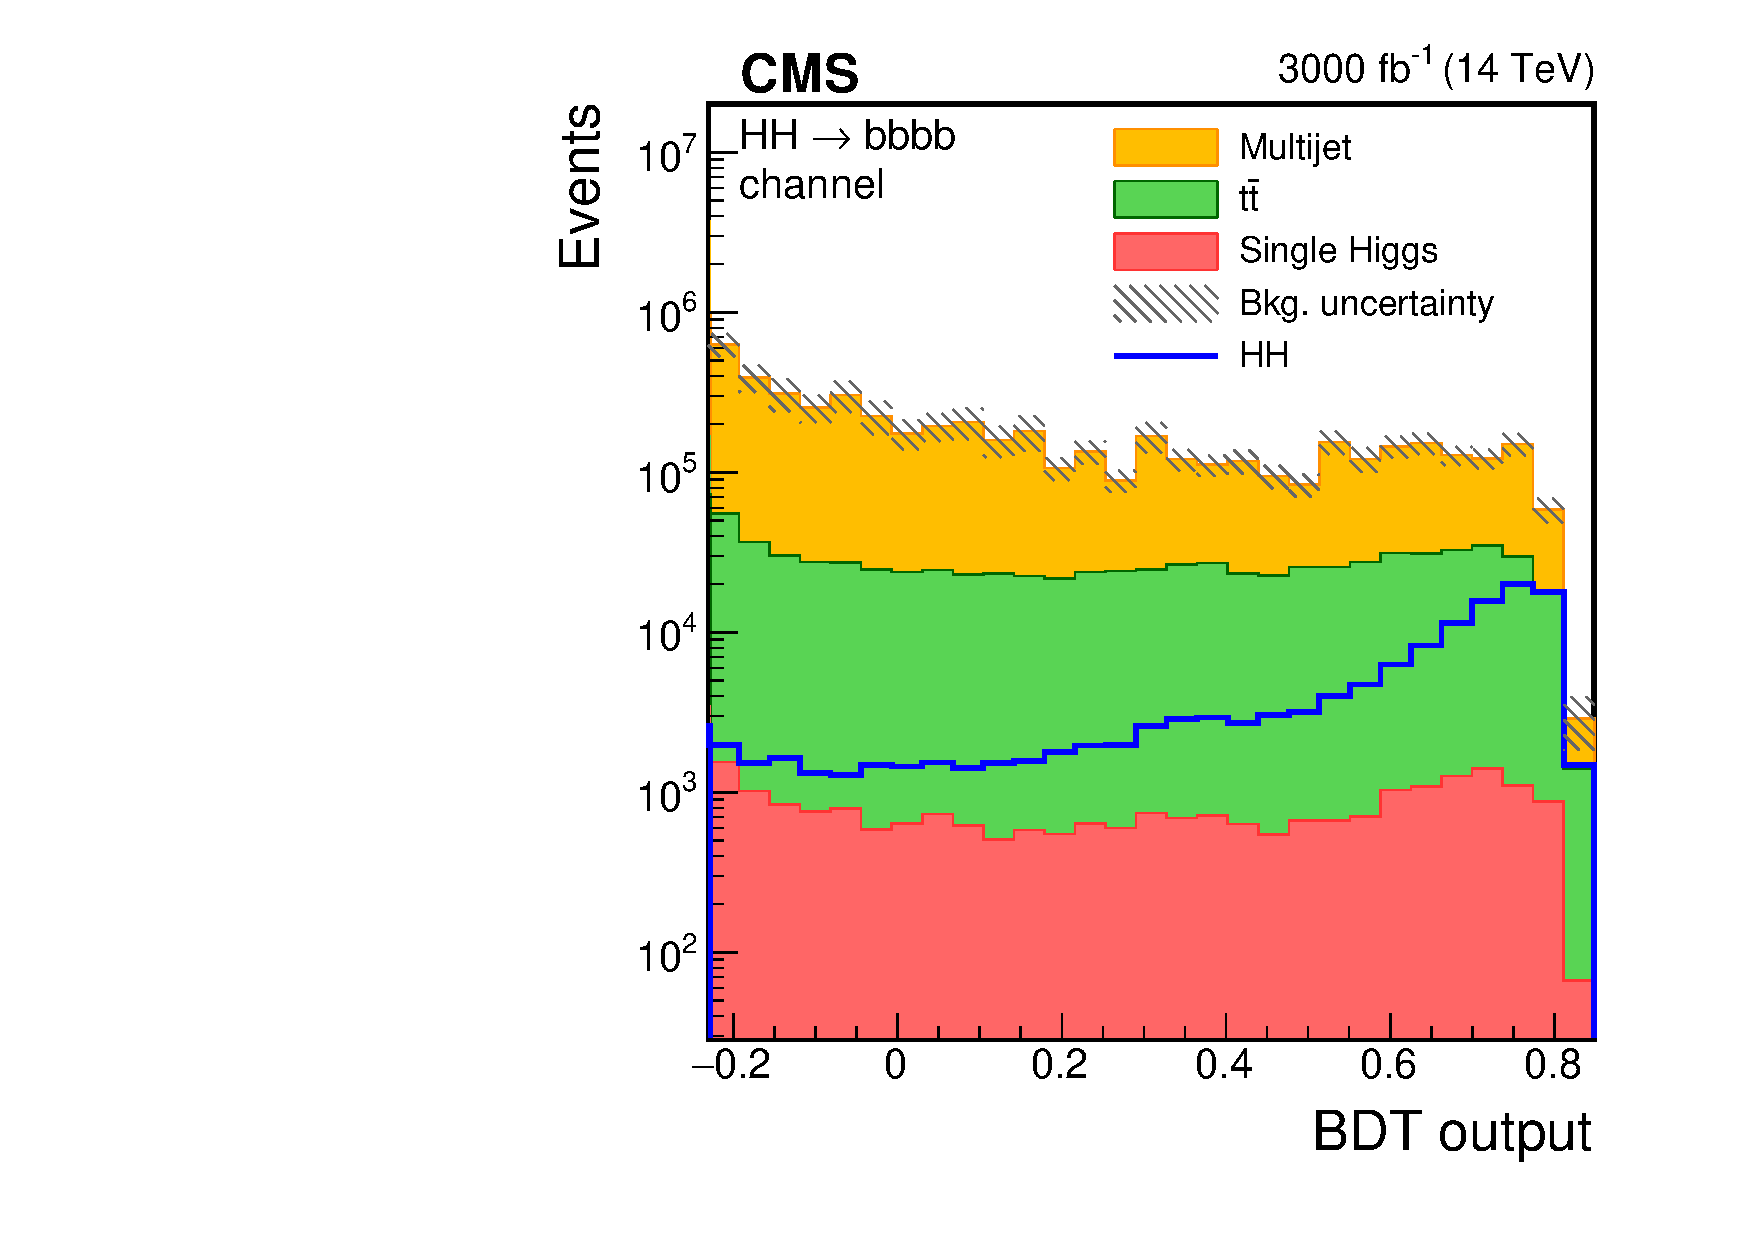
\includegraphics[width=0.5\textwidth]{\main/section3/plots/CMS/plot_BDTG_6_masscut_finalsel_log.pdf}
\caption{BDT output distribution for the signal and background processes considered in the \bbbb resolved search.} 
\label{sec3:CMSHH:fig:bbbb_BDT} 
\end{figure}

The boosted topology offers a good handle to investigate effective Higgs boson contact interactions predicted in BSM scenarios that enhance the \HH production cross section at high $m_{\HH}$ values.
For that reason, the prospects in this channels focus on anomalous couplings and make use of the shape benchmarks signals described in Ref.~\cite{Carvalho2016}.
Large radius jets, clustered with the anti-$k_\text{T}$ algorithm with a cone radius of 0.8 (AK8 jets), are used to identify the  overlapping b jets.
The event is required to contain at least two AK8 jets with $\pt > 300\GeV$ and $|\eta| < 3$.
The two highest $\pt$ jets are chosen in case multiple candidates satisfy such requirements.
The soft drop~\cite{Dasgupta:2013ihk,Larkoski:2014wba} jet grooming algorithm is used to remove soft and collinear components of the jet and retain the two sub-jets associated with the showering and hadronisation of the two b quarks from the $\PH\to\PQb\PAQb$ decay.
A selection is applied on the N-sub-jettiness variable~\cite{Thaler:2011gf} to reduce the background contamination, mostly represented by di-jet production from QCD interactions.
Algorithms for the b jet identification are applied on the sub-jets with a working point corresponding to an efficiency of about 49\% for genuine b jets for a mis-identification rate of light flavour and gluon jets of about 1\%.
Events are divided in two categories if they contain exactly three (3b category) or exactly four (4b category) b-tagged sub-jets.

The invariant mass of the two selected AK8 , $M_{JJ}$, is used to look for the presence of a signal. Its distribution is shown in Fig.~\ref{sec3:CMSHH:fig:bbbb_boosted} for the two event categories.

\begin{figure}[!htb]
\centering 
    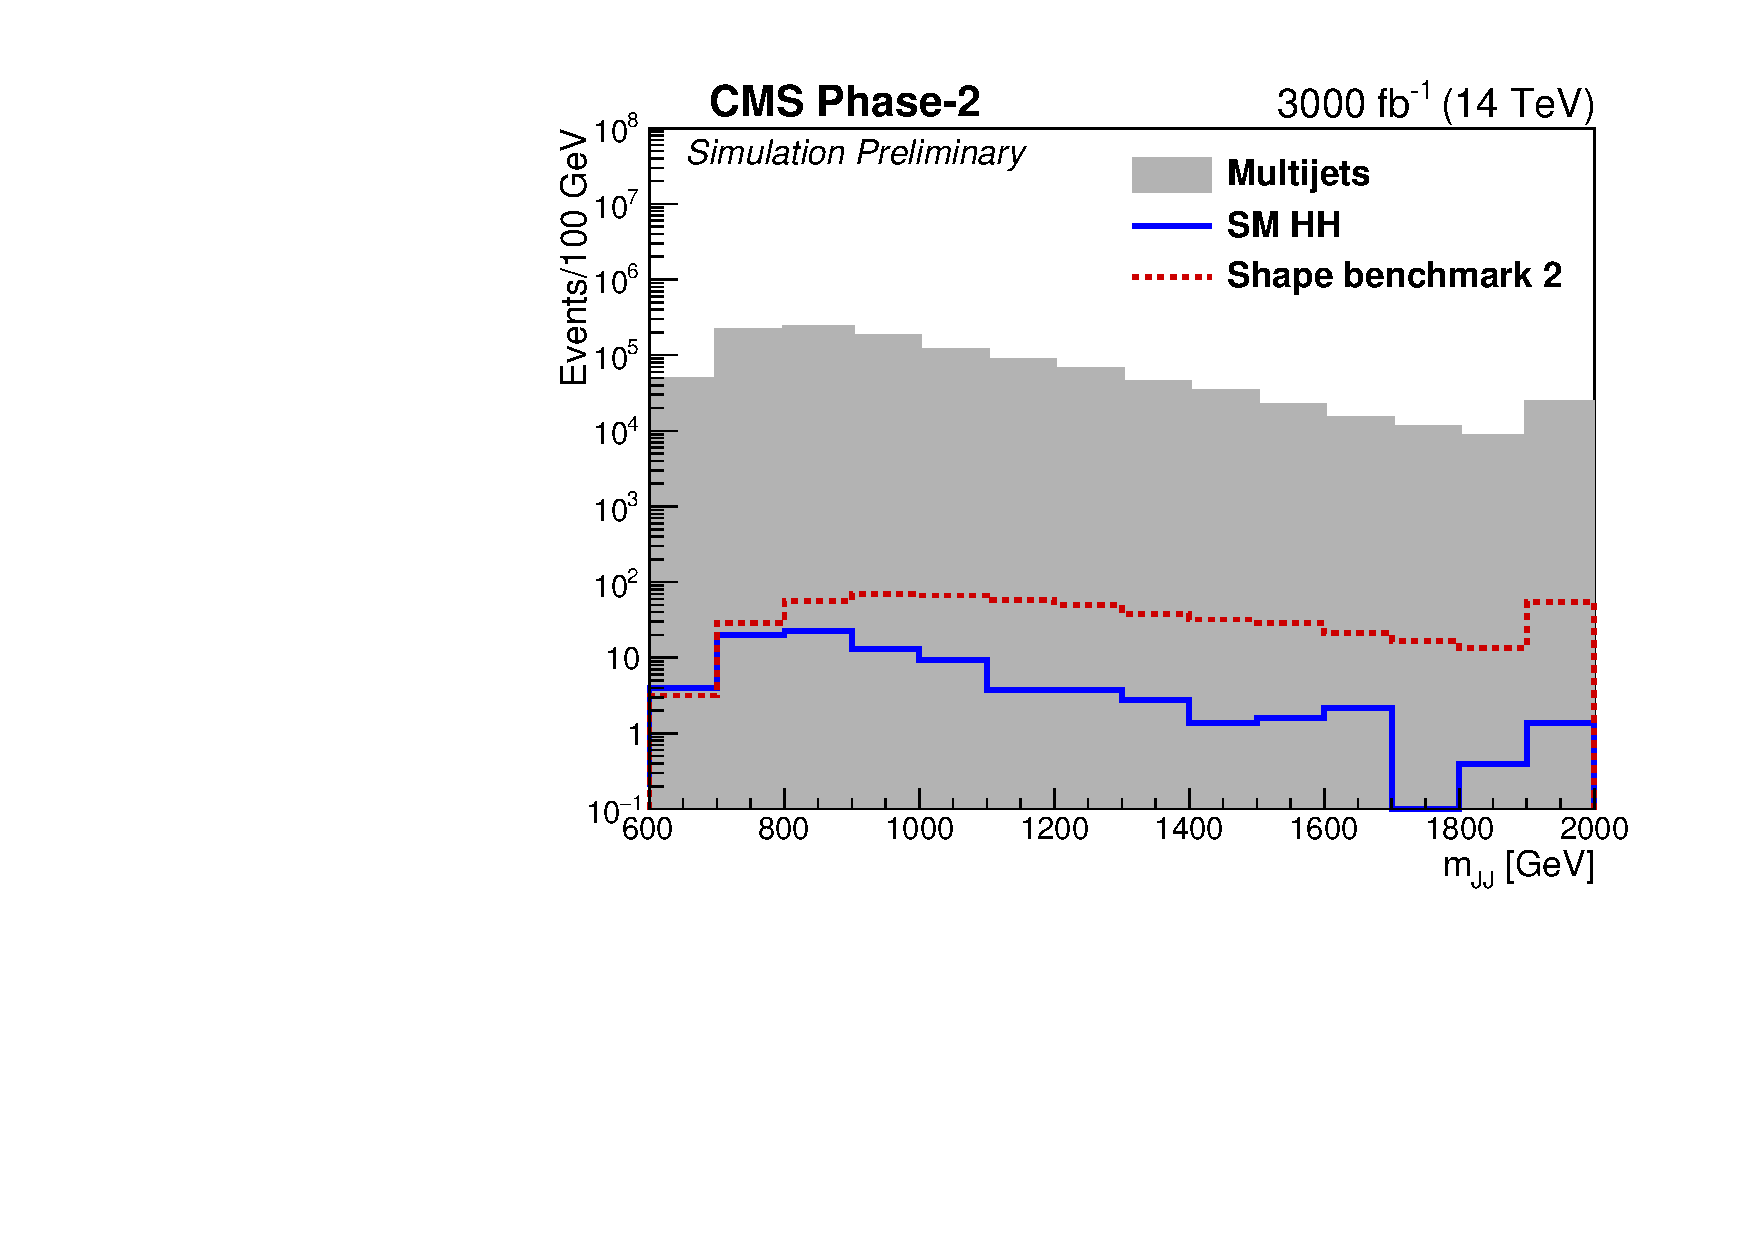
\includegraphics[width=0.495\textwidth]{\main/section3/plots/CMS/c_compare_h_mjj_3b_200_Logy1.pdf}
    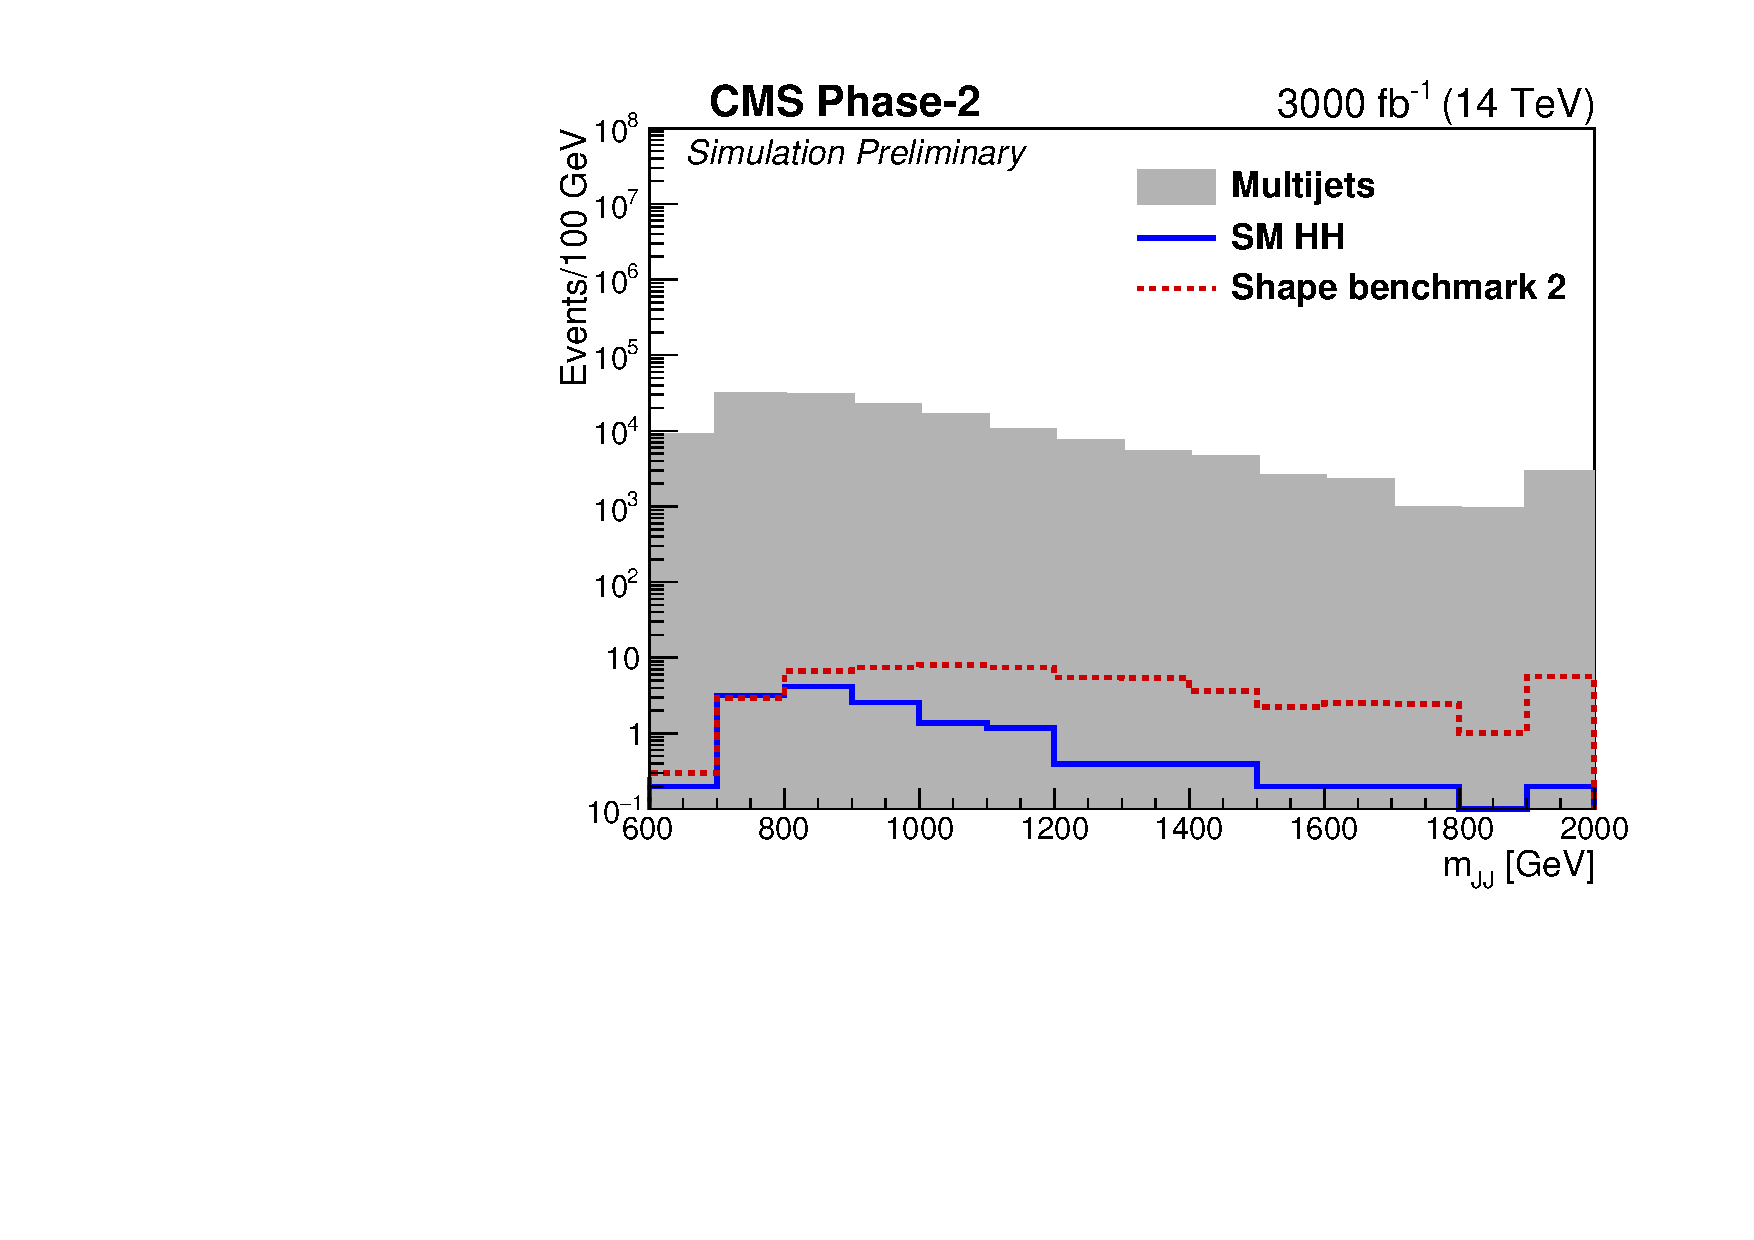
\includegraphics[width=0.495\textwidth]{\main/section3/plots/CMS/c_compare_h_mjj_4b_200_Logy1.pdf}
\caption{Invariant mass of the two selected AK8 jets in the boosted \bbbb \HH search for the multi-jet background and the SM (blue) and shape benchmark 2 (red) signals.
    The distributions on the left are for the $3\PQb$ and those on the right are for the $4\PQb$ sub-jet $\PQb$-tagged categories.
    Both signals are normalised to the SM $\PH\PH$ production cross section for visualisation.} 
\label{sec3:CMSHH:fig:bbbb_boosted} 
\end{figure}



\paragraph{The $HH \rightarrow \bbtt$ channel}

The $\bbtt$ decay channel is experimentally favourable thanks to its sizeable branching fraction of 7.3\% and the moderate background contamination.
Out of the six possible decay channels of the $\tau\tau$ system, the $\mu\tauh$, $\Pe\tauh$, and $\tauh\tauh$ final states are considered here, corresponding together to about 88\% of the total branching ratio.
Events in the three channels are selected requiring the presence of a \tauh candidate in association to an isolated muon, electron, or another \tauh\ depending on the final state considered.
Events in all the three categories above are then required to contain at least two b-tagged jets with $\pt > 30\GeV$ and $|\eta| < 2.4$. 

The main backgrounds are \ttbar and Drell-Yan production of $\tau$ pairs.
Their separation is experimentally challenging because of the incomplete reconstruction of the event due to the presence of neutrinos from $\tau$ decays that escape detection.

A multivariate analysis method is thus used to identify the signal contribution and separate if from the large background.
The usage of state-of-the-art machine learning techniques is studied in this work.
The discriminant consists of a pair of ensembles of ten fully connected deep neural networks (DNN), each with three hidden layers of 100 neurons, trained to separate the \HH signal from the background processes using a wide set of kinematic variables, a few of which are shown for illustration in Fig.~\ref{sec3:CMSHH:fig:bbttinputs}.
Each network is trained using events from all three $\tau\tau$ decay channels, and advanced optimisation techniques are explored and applied to maximise the expected sensitivity.

\begin{figure}[!htb]
\centering 
    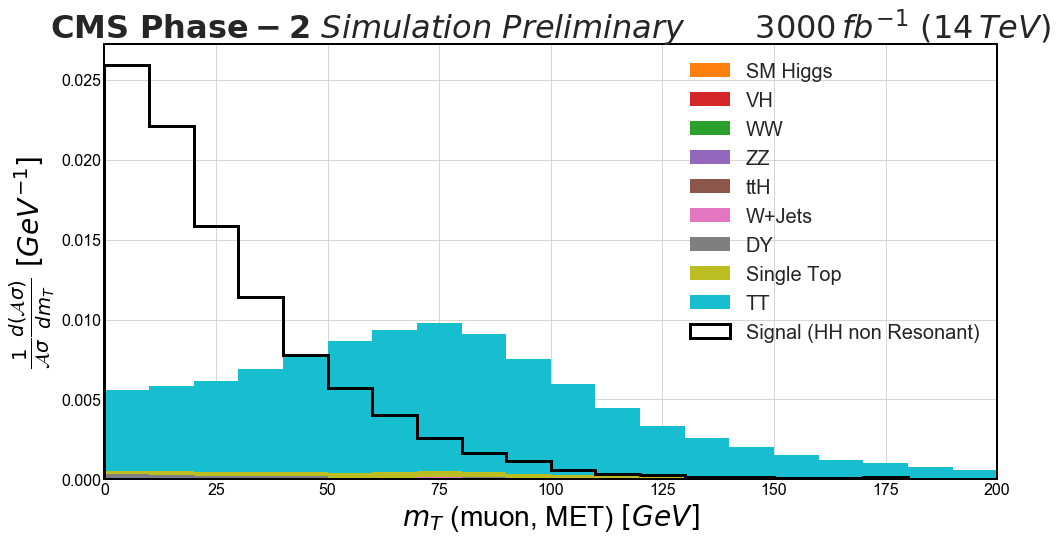
\includegraphics[width=0.495\textwidth]{\main/section3/plots/CMS/figure5a.png}
    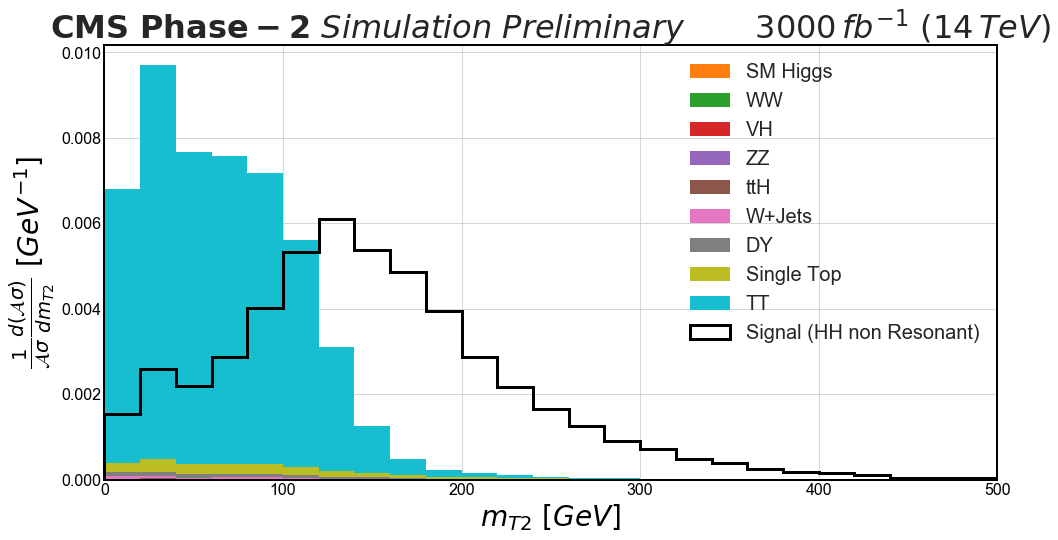
\includegraphics[width=0.495\textwidth]{\main/section3/plots/CMS/figure5e.png}\\
    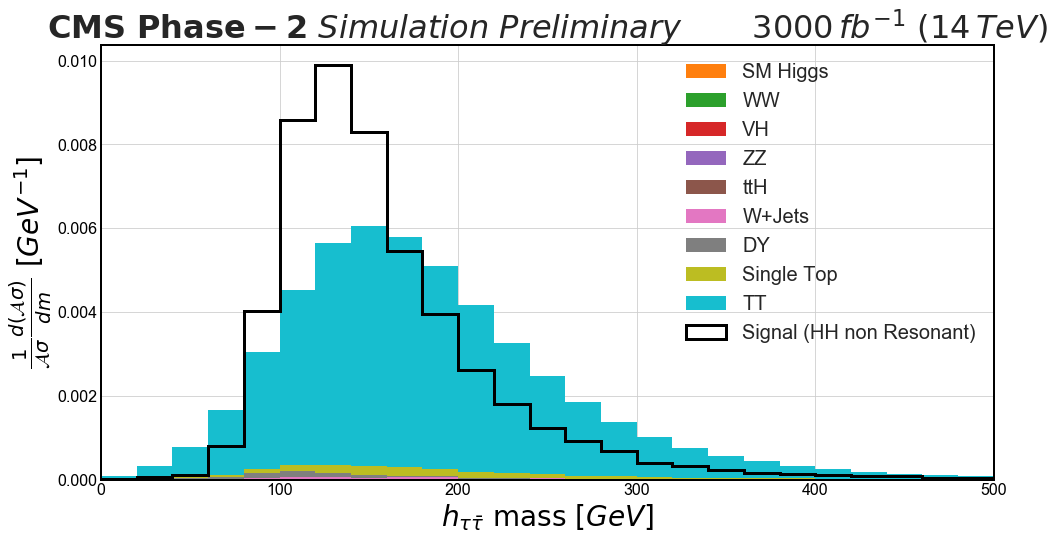
\includegraphics[width=0.495\textwidth]{\main/section3/plots/CMS/figure5c.png}
    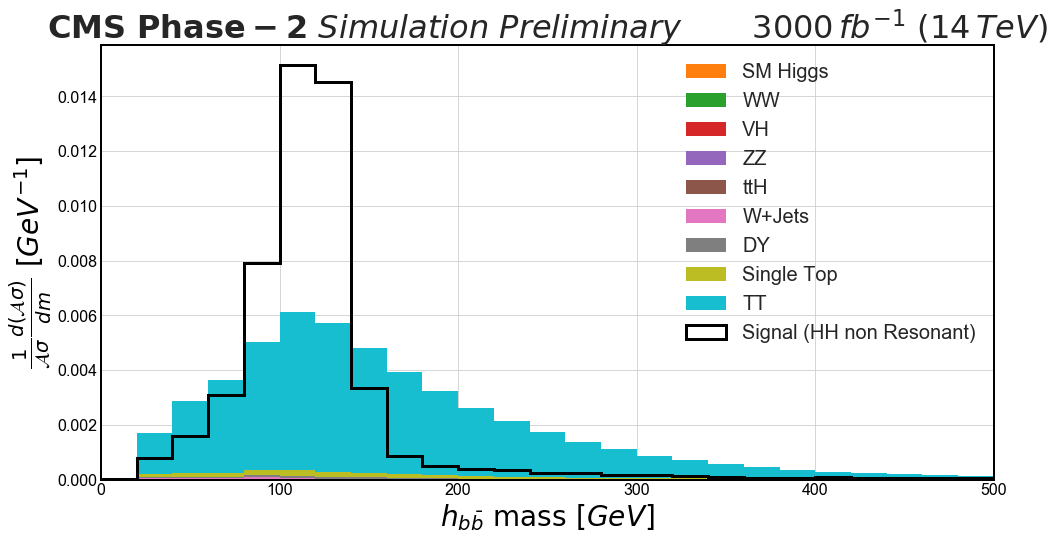
\includegraphics[width=0.495\textwidth]{\main/section3/plots/CMS/figure5d.png}\\    
\caption{Example distributions for some of the discriminant variables used as input of the \bbtt deep neural network for the $\mu\tauh$ final-state: muon transverse mass (top left), system transverse mass $m_\text{T2}$ (top right), and invariant mass of the $\tau\tau$ (bottom left) and bb (bottom right) systems.} 
\label{sec3:CMSHH:fig:bbttinputs} 
\end{figure}


\paragraph{The $HH \rightarrow b\bar{b}\gamma\gamma$ channel}

Despite its low branching fraction, the \bbgg decay channel is one of the most sensitive to \HH production.
It benefits of an excellent di-photon invariant mass ($m_{\gamma\gamma}$) resolution and on the possibility to fully reconstruct all final state objects.
The analysis strategy combines these two aspects and uses a multivariate kinematic discriminant to suppress the background contributions, and the $m_{\gamma\gamma}$ signature to look for the presence of a signal.

The $\PH\to\gamma\gamma$ candidate is built from two photons in the collision event that satisfy identification, isolation, and quality criteria.
Only events where the two photons satisfy $|\eta| < 2.5$ and $100 < m_{\gamma\gamma} < 150$ are considered.
%The photons are  $p_{T,1} > m_{\gamma\gamma}/3$~GeV and $p_{T,2} > m_{\gamma\gamma}/4$~GeV and $|\eta| <$ 2.5 are selected  and we constraint $ 100 < m_{\gamma\gamma} < 150$~GeV. Fiducial region between the barrel and endcap calorimeters is rejected. For this selection defined as is Run II \cite{???} the trigger is expected to be fully efficient.
%The working point chosen for photon identification and isolation selects about 90\% of photons within the required kinematic region. 
The $\PH\to\text{bb}$ candidate is built from the two highest $\pt$ jets that satisfy $\pt > 25\GeV$ and $|\eta| < 2.5$.
%The Phase II tracker allows to extend the b-tagging region up to $|\eta| = 4$, but the impact on this analysis is very limited.
The background from light flavour jets is suppressed by requiring both jets to satisfy a loose working point of the  b tagging algorithm, corresponding to a 90\% efficiency for a genuine b-jet and 10\% mis-identification rate.
The di-jet invariant mass is required to be between 80 and 190\GeV. 

The backgrounds mainly consist of non-resonant $\gamma\gamma$ production in association with heavy flavour jets, with a smaller contribution from $\gamma\gamma$ plus light flavour jets, and single Higgs boson production in association with top quark ($\Ptop\Ptop\PH$, with $\PH\to\gamma\gamma$).
%A contribution of $\approx$ 10\% of the events is expected, for the photon identification working point chosen in this analysis, from 
%$\gamma$ jet $+ 2$~jets where a jet is identified as photon 

A multivariate discriminant  in the form of a BDT is used to suppress the $\Ptop\Ptop\PH$ background.
%This latter contribution is the dominant source of single $H \rightarrow \gamma\gamma$ background that have the same properties than HH production for the main discriminating variable $m_{\gamma\gamma}$.
The BDT is trained to identify the presence of decay products from $\PW$ bosons originating from top quark decays, and combines the information on the presence and properties of leptons, additional jets, and helicity angles of the $\HH$ system and its decay products.
A selection on the discriminant is applied, rejecting approximately 75\% of the $\Ptop\Ptop\PH$ events for a 90\% signal efficiency.

A second BDT classifier is trained to separate the $\HH$ signal from the non-resonant di-photon background.
Several variables related to the kinematic properties of the event and to the quality of the selected objects are combined, and background-like events with a low BDT scores are rejected.

Events thus selected are simultaneously classified based on the value of the BDT discriminant described above and on the reduced mass of the four objects selected, defined as:
\begin{equation}
    M_\text{X} = m_{\gamma\gamma\text{jj}} - m_{\gamma\gamma} - m_\text{jj} + 250\GeV,
\end{equation}
where $m_{\gamma\gamma\text{jj}}$, $m_{\gamma\gamma}$, and $m_\text{jj}$ refer respectively to the four body, di-photon, and di-jet invariant masses.
The definition of $M_\text{X}$ mitigates resolution effects by using the expected Higgs boson mass.
Two intervals of the BDT scores are used to define medium and high purity categories (MP and HP), and events in each category are further divided in a low, medium, and high mass category if $250 < M_\text{X} < 350\GeV$, $350 < M_\text{X} < 380\GeV$, or $480 < M_\text{X}~\GeV$, respectively.
While the high mass category is the most sensitive to SM \HH production, low mass categories are important to constrain anomalous values of the Higgs boson self-coupling, that enhance the cross section at the $m_{\HH}$ threshold.

The signal is extracted from a simultaneous fit in each of the $3 \times 2$ categories defined above.
A parametric maximum likelihood fit of the signal and background in the $(m_{\gamma\gamma}, m_\text{jj})$ is used.
An example of the expected event distributions in the high mass and high purity category for the two variables is shown in Fig.~\ref{sec3:CMSHH:fig:bbgg_events}.

\begin{figure}[!htb]
\centering 
    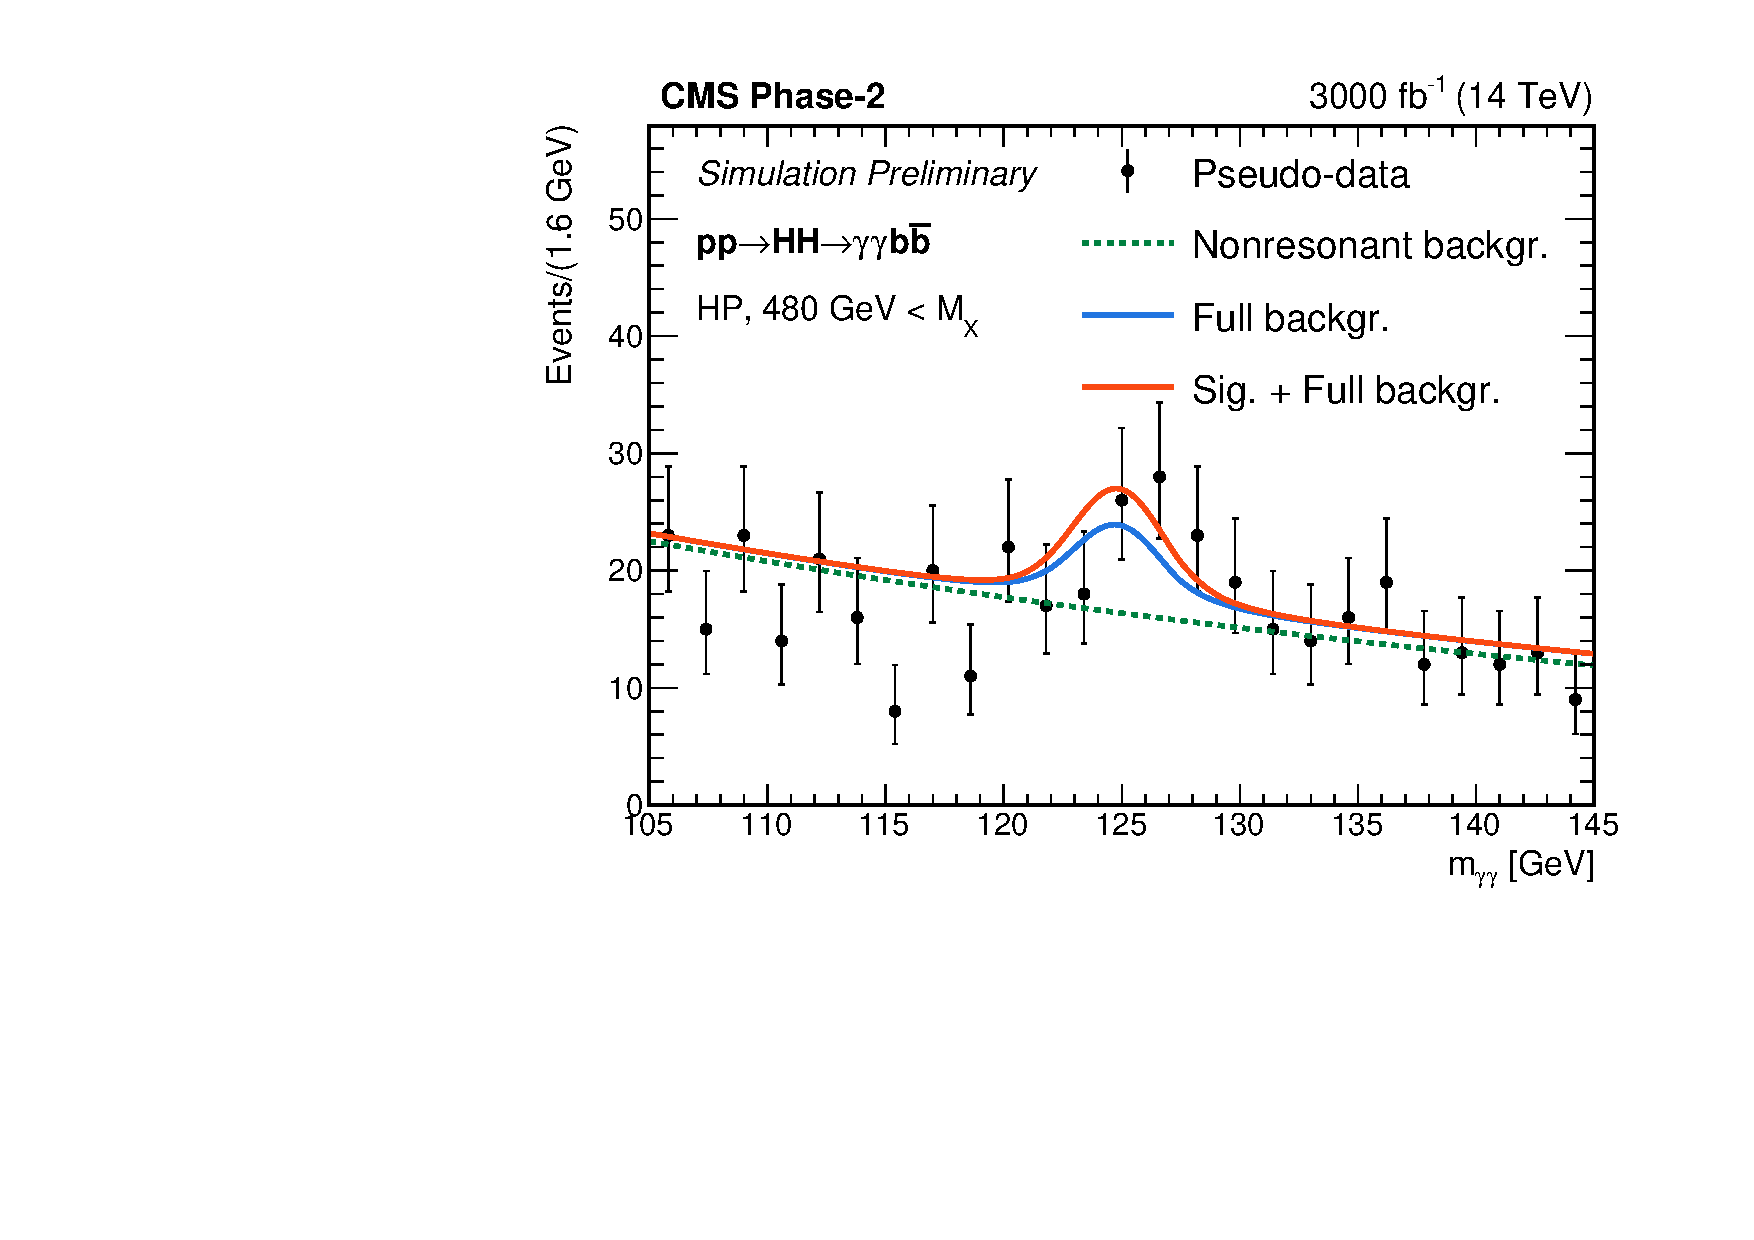
\includegraphics[width=0.495\textwidth]{\main/section3/plots/CMS/Cat4_mgg_poiss.pdf}
    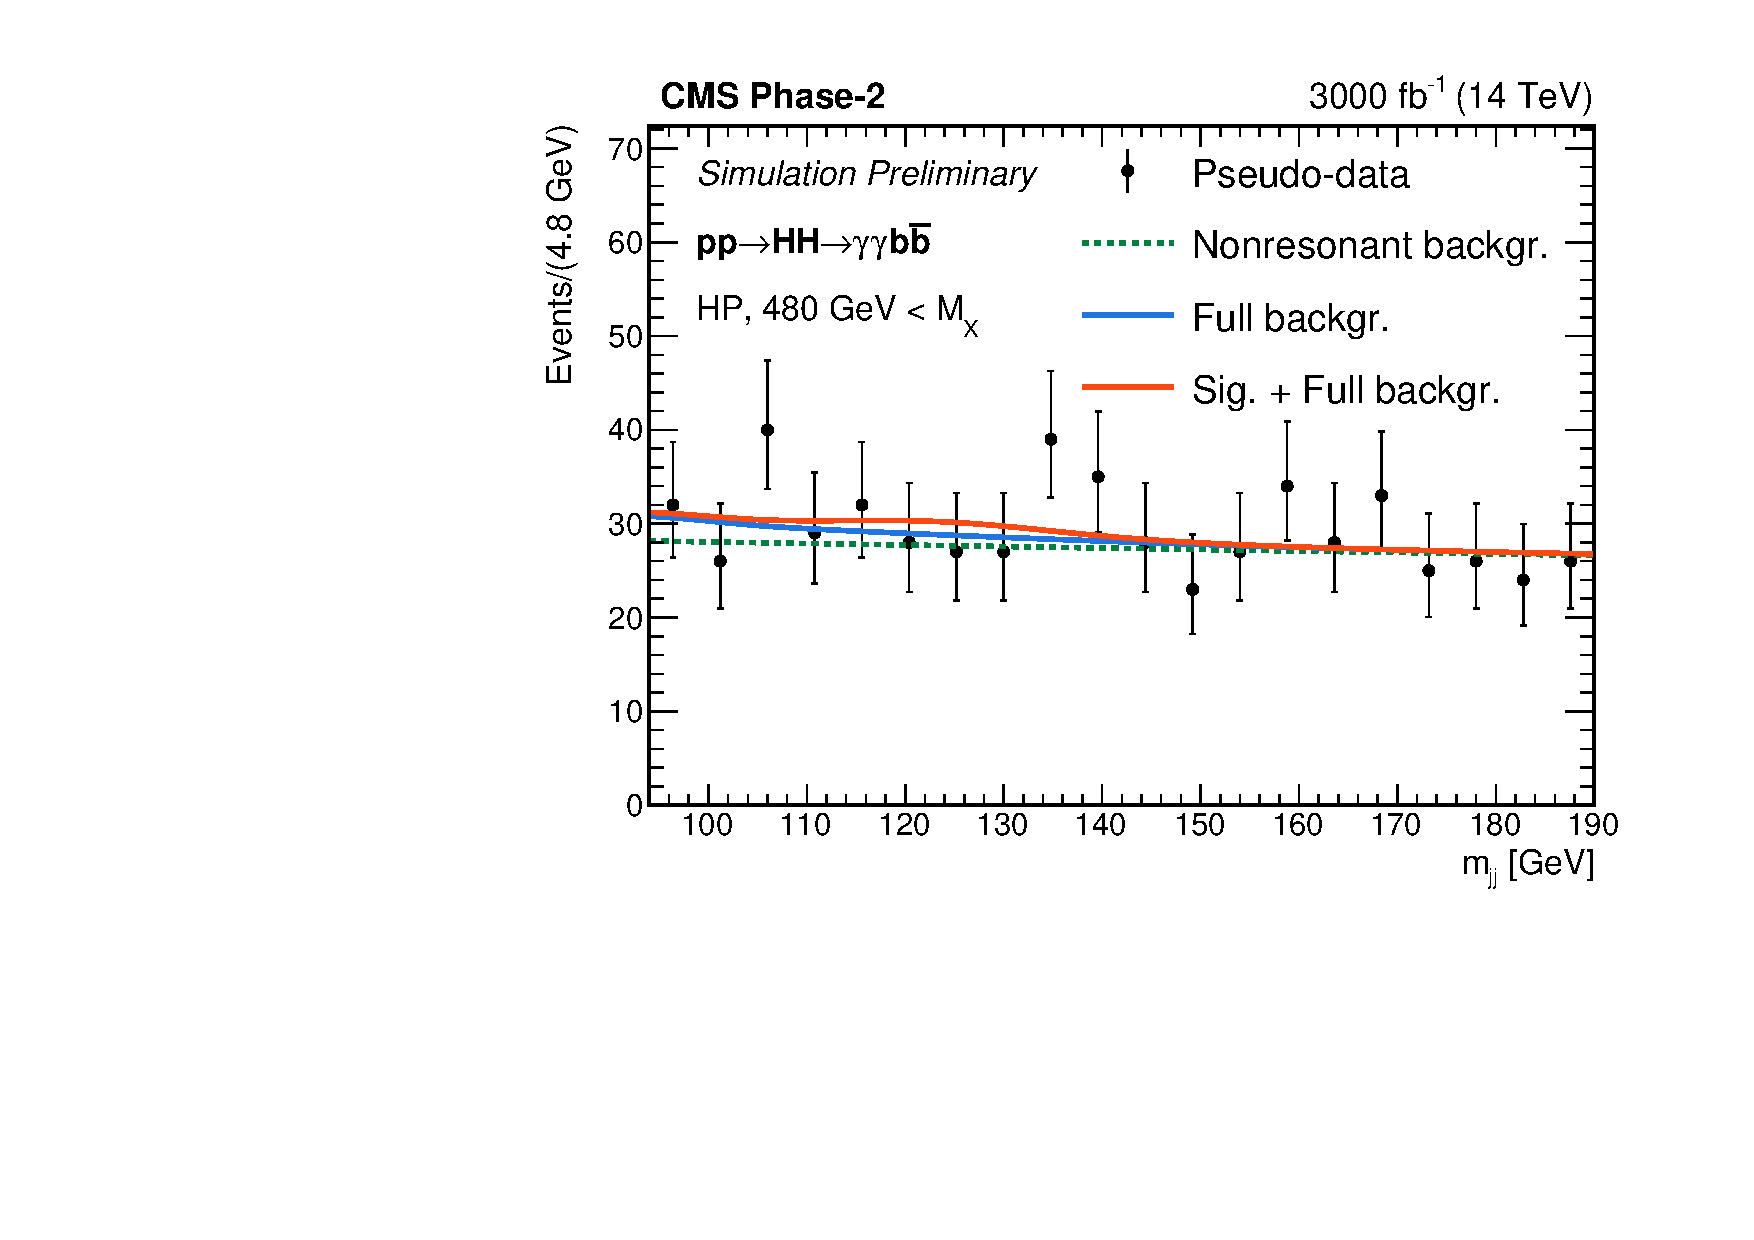
\includegraphics[width=0.495\textwidth]{\main/section3/plots/CMS/Cat4_mjj_poiss.pdf}
\caption{Expected distribution of events in the photon (left column) and jet (right column) pair invariant mass for the high mass and high purity event category. The full circles denote pseudo-data obtained from the expected events yields for the sum of the signal and background processes for $3000\fbinv$.} 
\label{sec3:CMSHH:fig:bbgg_events} 
\end{figure}

\paragraph{The $HH \rightarrow \bbWW \to \PQb\PQb\ell\nu\ell\nu$ channel}

We consider here \HH final states containing two \PQb jets  and two neutrinos and two leptons, either electrons or muons.
The decay channels involved are thus $\PH\to\bb$ in association with either a $\PH\to\PZ(\ell\ell)\PZ(\nu\nu)$ or a $\PH \to \PW(\ell\nu)\PW(\ell\nu)$ decay.
While the analysis described in the following is optimised for $\HH\to\bbWW$ decays, that provide the largest branching fraction, the contribution of Higgs boson decays to both $\PW\PW$ and $\PZ\PZ$, globally denoted as $\text{VV}$, is considered.
Decays of the $\text{VV}$ system to tau leptons subsequently decaying to electrons or muons with the associated neutrinos are also considered in the simulated signal samples.
The corresponding branching fraction for the $\text{VV}\to\ell\nu_\ell\ell\nu_\ell$ decay is 1.73~\%.

The dominant and sub-dominant background processes are
the $\ttbar$ production in its fully leptonic decay mode, and
Drell-Yan production of lepton pairs in association with jets.
As both are irreducible background processes, \ie they result in the same final state as the signal, the kinematic properties of the signal and background events are used and combined in an artificial Neural Network (NN) discriminant to enhance the sensitivity.

Events are required to contain two isolated leptons of opposite electric charge, with an invariant mass $m_{\ell\ell} > 12
\UGeV$ to suppress leptonia resonances and $m_{\PZ} - m_{\ell\ell} > 15\GeV$ to suppress Drell-Yan lepton pair production.
The $\PH\to\PQb\PQb$ decay is reconstructed by requiring the presence of two b-tagged jets in the event with $\pt > 20$~\UGeV and $| \eta | < 2.8$, separated from the selected leptons by a distance of $\Delta \text{R} = \sqrt{\Delta \phi^2 + \Delta \eta^2} > 0.3$.

% Events are required to contain two leptons of opposite electric charge
% ($\Pe^{+}\Pe^{-}, \mu^{+}\mu^{-}, \Pe^{\pm}\mu^{\mp}$), and with \pt greater than 25~GeV and 15~GeV for
% $\Pe\Pe$ events, 20~GeV and 10~GeV for $\mu\mu$ events, 25~GeV and 15~GeV for
% $\mu\Pe$ events, 25~GeV and 10~GeV for $\Pe\mu$ events, for the higher and lower \pt lepton,
% respectively. Electrons and muons in the pseudo-rapidity range
% $| \eta | < 2.8$ are considered, except the $ 1.444 < | \eta | < 1.5666$ being rejected for electrons.
% A dilepton mass requirement of $m_{\ell\ell} > 12$~GeV is applied to all flavour combinations in
% order to suppress lepton onia resonances.


% Jets are required to have
% $\pt > 20$~GeV, $| \eta | < 2.8$, and be separated from identified leptons
% by a distance of $\Delta \text{R} = \sqrt{\Delta \phi^2 + \Delta \eta^2} > 0.3$.
% The magnitude of the negative vector sum of all PF candidates is referred
% to as $\ptmiss$. 
% Selected jets must also satisfy the medium working point of the b tagging algorithm.

% A neural network (NN) discriminant is used to improve the signal-to-background
% separation.
The NN discriminant utilises information related
to object kinematics.
The variables provided as input to the NN exploit the presence of two Higgs  bosons decaying into two b-jets on the one hand, and two leptons and two neutrinos on the other hand, 
which results in different kinematics for the di-lepton and di-jet systems between signal and 
background processes.
The set of variables used as input is:$ m_{\ell\ell}$, $m_\text{jj}$,
$\Delta R_{\ell\ell}$, $\Delta R_{\text{j}\text{j}}$, $\Delta \phi_{\ell\ell, \text{j}\text{j}}$, defined as 
the $\Delta \phi$ between the di-jet and the di-lepton systems, $\pt^{\ell\ell}$, $\pt^{\text{j}\text{j}}$,
min$\left(\Delta R_{\text{j}, \ell}\right)$, and $\mathrm{M}_\mathrm{T}$, defined as
$\mathrm{M}_\mathrm{T} = \sqrt{2 \pt^{\ell\ell} \ptmiss (1 - \cos(\Delta \phi(\ell\ell, \ptmiss)))}$.

The output of the NN is used as the discriminant variable in the three decay channels studied, and its distribution is reported in Fig.~\ref{sec3:CMSHH:fig:bbWW_events}.

\begin{figure}[!htb]
  \begin{center}
    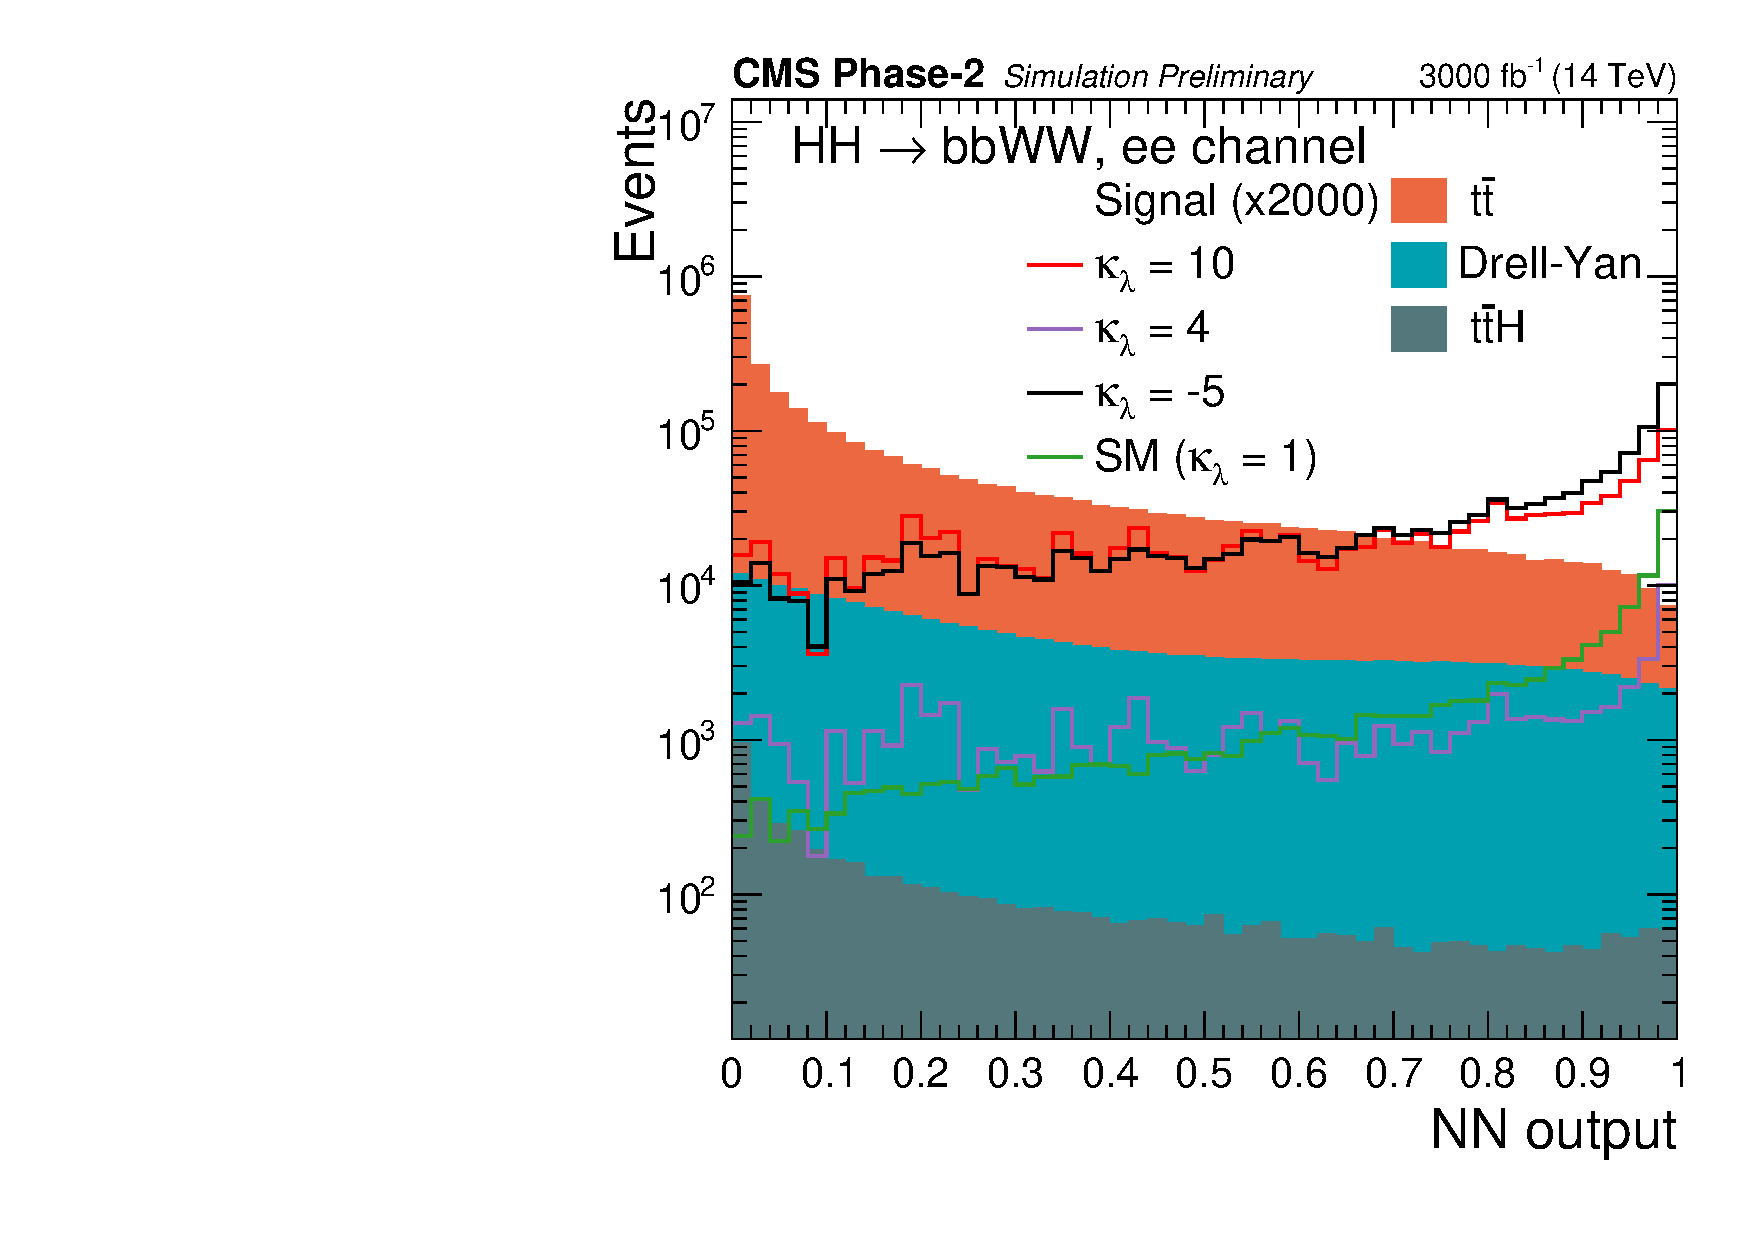
\includegraphics[width=0.32\textwidth]{\main/section3/plots/CMS//NN_nonresonant_point_1p00_1p00_ElEl_hh_llmetjj_HWWleptons_btagM_cmva_mll_cut_rebin_final_logy.pdf}
    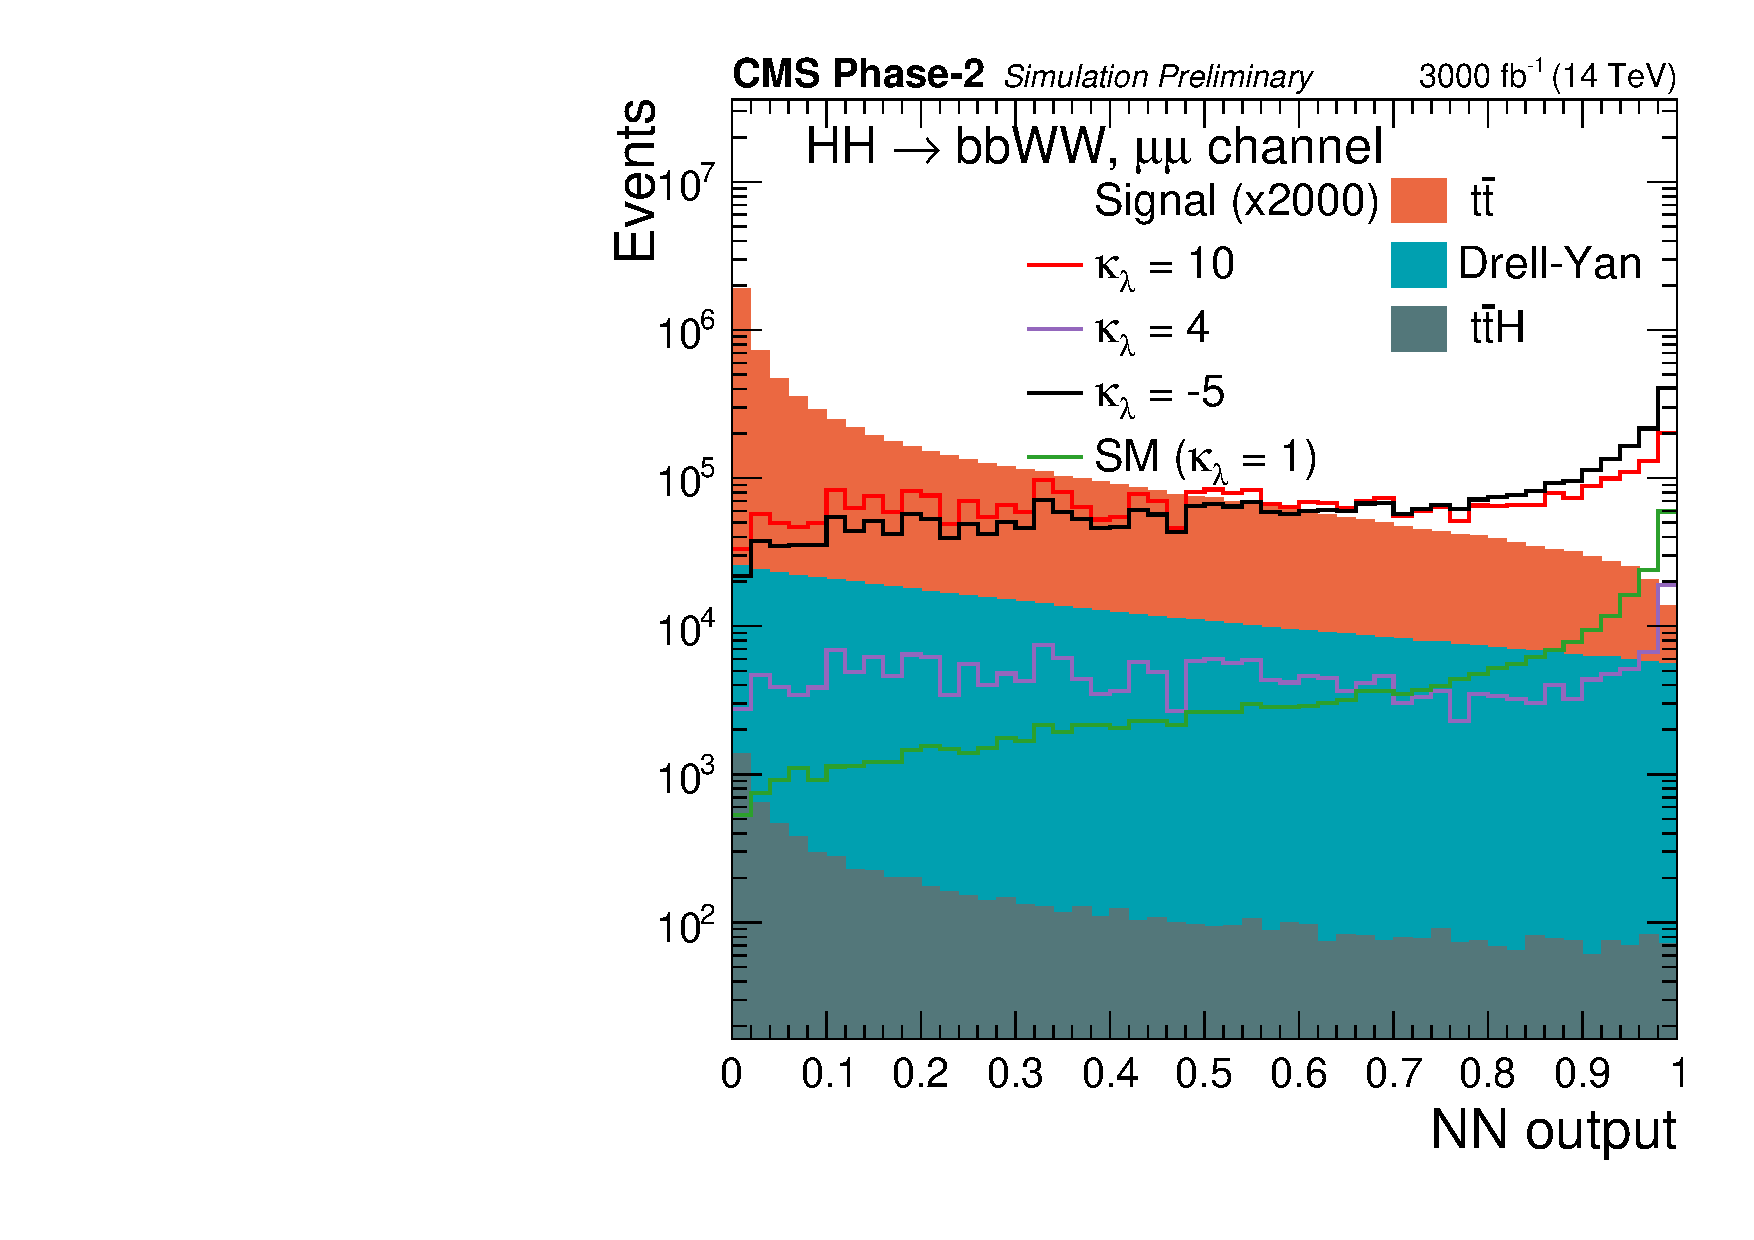
\includegraphics[width=0.32\textwidth]{\main/section3/plots/CMS//NN_nonresonant_point_1p00_1p00_MuMu_hh_llmetjj_HWWleptons_btagM_cmva_mll_cut_rebin_final_logy.pdf}
    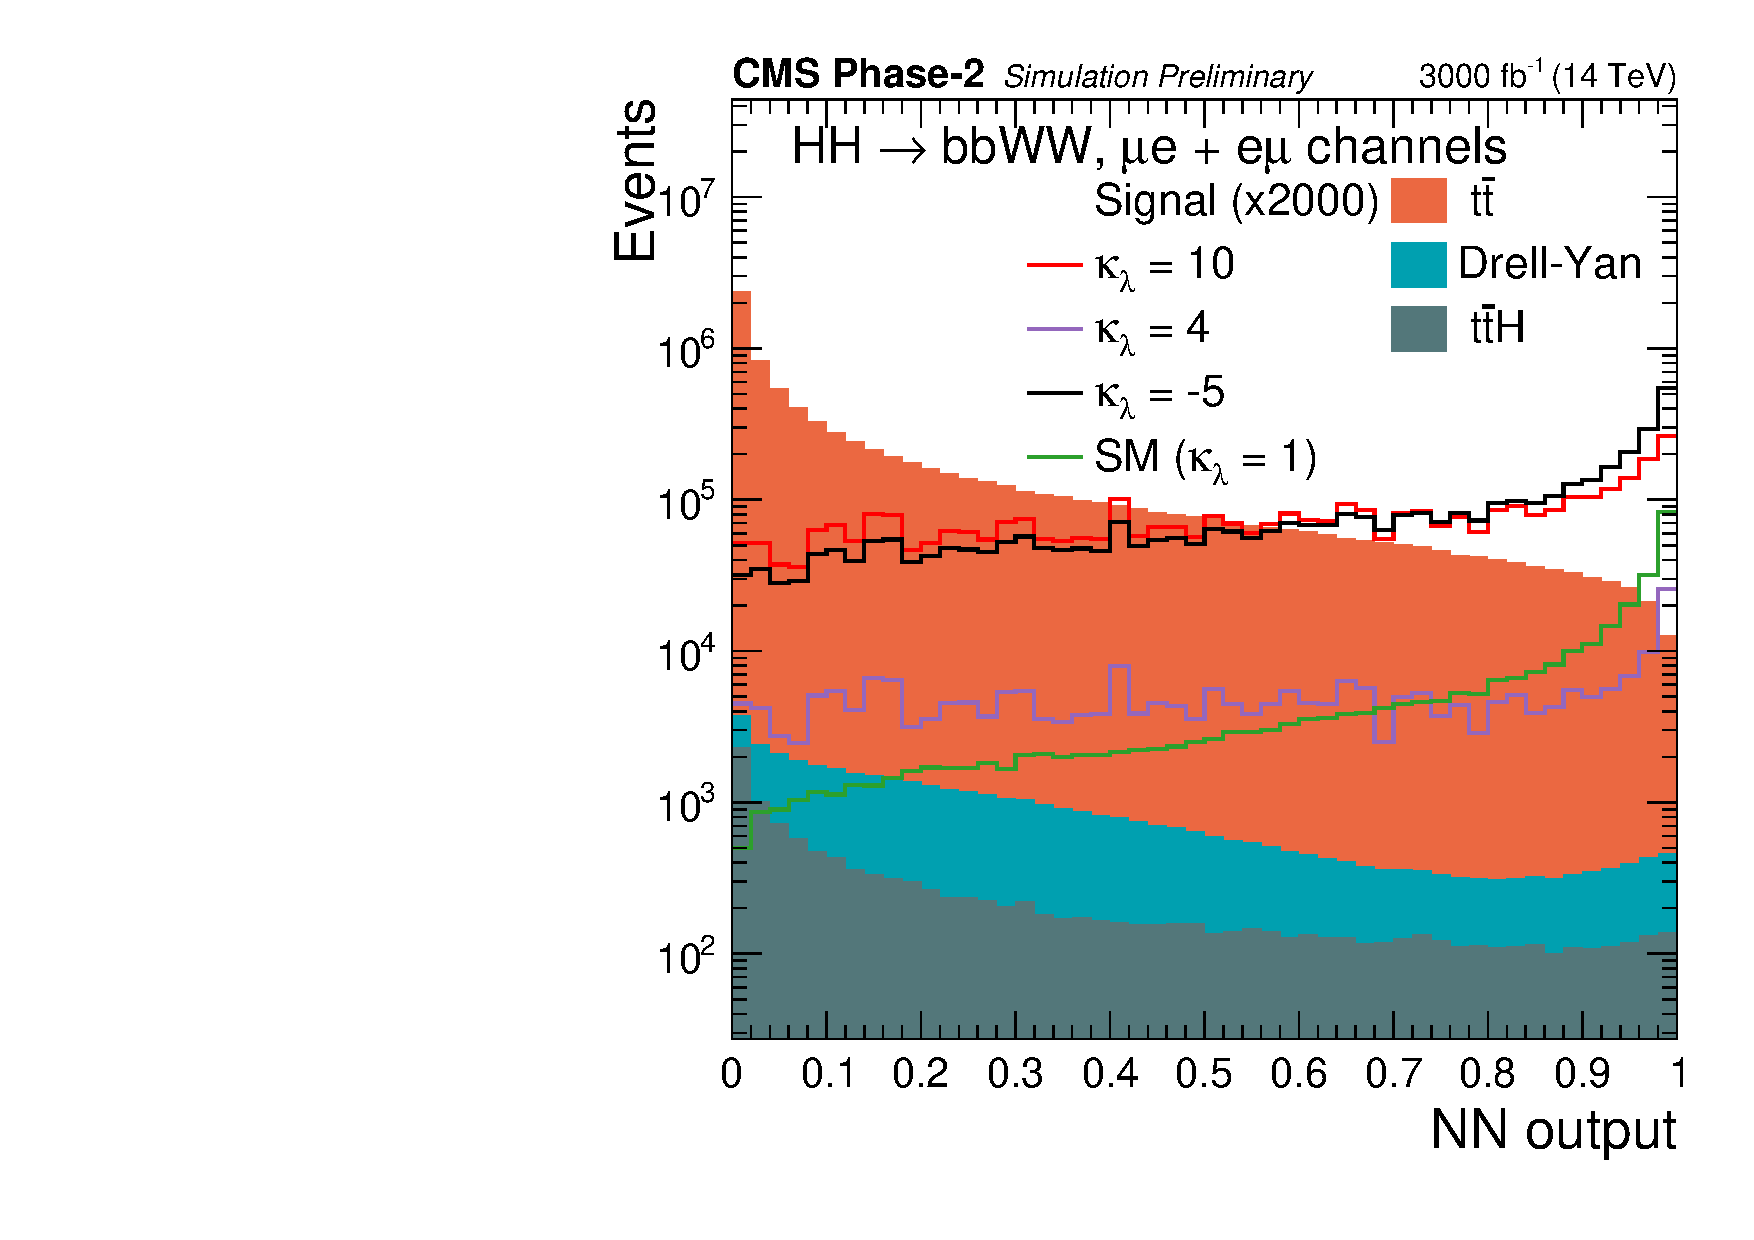
\includegraphics[width=0.32\textwidth]{\main/section3/plots/CMS//NN_nonresonant_point_1p00_1p00_MuEl_hh_llmetjj_HWWleptons_btagM_cmva_mll_cut_rebin_final_logy.pdf}
    \caption{
      The output of the $\bbWW$ NN after the selections, evaluated in the
      $\Pe^{+}\Pe^{-}$~(left) , $\mu^{+}\mu^{-}$~(middle),
      $\Pe^{\pm}\mu^{\mp}$~(right) channels.
    }
    \label{sec3:CMSHH:fig:bbWW_events}
  \end{center}
\end{figure}


\paragraph{The $\HH\to\bbZZ\to \PQb\PQb 4\ell$ channel}

The \HH searches at the LHC have so far focused on final states with a sizeable branching ratio because of the small cross section of this process.
The HL-LHC will open the possibility to study rare but clean decay channels thanks to the large dataset available.
The $\bbZZ(4\ell)$ channel, that is investigated in this work, benefits from the clean four lepton signature to clearly identify signal events in the busy pileup environment of the HL-LHC.

Events are required to have at least four identified and isolated (isolation < 0.7) muons (electrons) with $\pt > 5(7)\GeV$ and $|\eta|< 2.8$. 
The two $\PZ$ boson candidates are formed from pairs of opposite-charge leptons
The $\PZ$ candidate with the invariant mass closest to the nominal Z mass is denoted as $\PZ_1$, while the other one is labelled as $\PZ_2$.
$\PZ$ candidates are required to have an invariant mass in the range [40, 120] \UGeV ($\PZ_1$) and [12, 120] \UGeV ($\PZ_2$), respectively.
%At least one lepton is required to have $p_T >$ > 20 GeV and a second is required to have $p_T >$ > 10 GeV.
%On figure~\ref{fig:CMS_HH4l} we show the resolution of the reconstructed $H \rightarrow ZZ \rightarrow 4l$ after baseline selections.
The four leptons invariant mass is requested to be in the range [120,130] \UGeV.
At least two (but not more than three) b-tagged jets are also required to be  present  and have an invariant mass.
The jet pair is required to have an invariant mass in the range [80, 160] \UGeV and an angular distance between the 2 jets between 0.5 and 2.3.
The number of events thus selected are used to look for the presence of a signal on top of the background processes, mostly constituted of single Higgs boson production in the $4\ell$ final state.
The distribution of the four lepton invariant mass is shown in  Fig,~\ref{sec3:CMSHH:fig:bbZZ_events}.


\begin{figure}[!htb]
  \begin{center}
    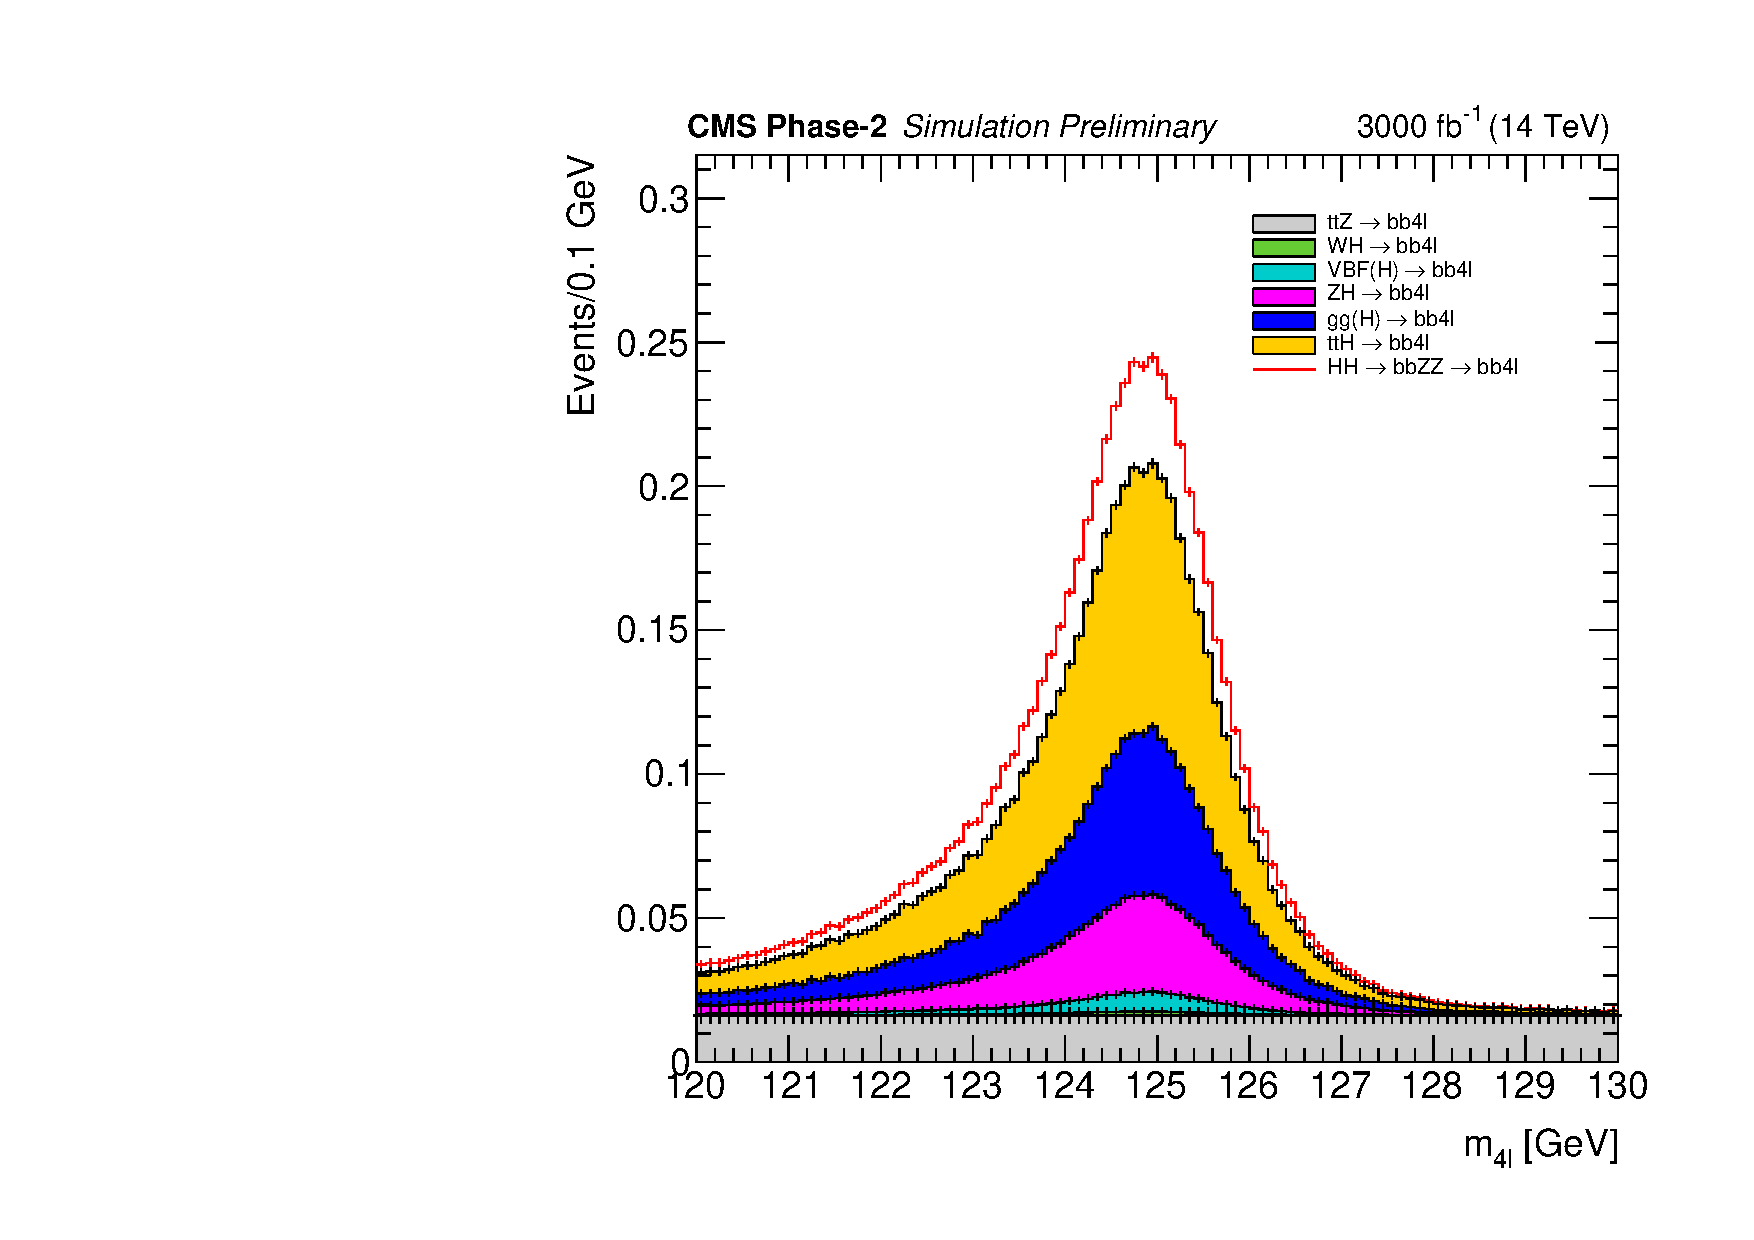
\includegraphics[width=0.49\textwidth]{\main/section3/plots/CMS/Mass_4l.pdf}
    \caption{Invariant mass distribution of the four leptons selected at the end of the analysis for the $\PQb\PQb 4\ell$ final state.}
    \label{sec3:CMSHH:fig:bbZZ_events}
  \end{center}
\end{figure}


\paragraph{Combined results}

The five decay channels are combined statistically assuming the SM Higgs boson branching fractions.
Assuming the presence of a signal with the properties predicted by the SM, its total expected  significance is $2.6\sigma$.
If instead the background only hypothesis is assumed, an expected upper limit on the SM \HH signal cross section can be set to 0.77 times the SM prediction.
The contributions from the five decay channels and the combined expected sensitivities are reported in Tab.~\ref{sec3:cMSHH:tab:comb}.

\begin{table}[htp]
\centering
\caption{Upper limit at the 95\% confidence level, significance, projected measurement at 68\% confidence level of the Higgs boson self coupling $\lambdahhh$ for the five channels studied and their combination. Systematic and statistical uncertainties are considered.}
\label{sec3:cMSHH:tab:comb}
\begin{tabular}{l c c c c}
    \toprule
    \multirow{2}{*}{Channel} & \multicolumn{2}{c}{Significance} & \multicolumn{2}{c}{95\% CL limit on $\sigma_{\HH}/\sigma_{\HH}^\text{SM}$} \\
    % \cmidrule(lr){2-3}
    % \cmidrule(lr){4-5}
                             & Stat. + syst.  & Stat. only &  Stat. + syst. & Stat. only \\
    \cmidrule(lr){2-3}
    \cmidrule(lr){4-5}
    % \midrule
    \bbbb                     & 0.95 & 1.2  & 2.1  & 1.6 \\
    \bbtt                     & 1.4  & 1.6  & 1.4  & 1.3 \\
    $\bbWW(\ell\nu\ell\nu)$   & 0.56 & 0.59 & 3.5  & 3.3 \\
    \bbgg                     & 1.8  & 1.8  & 1.1  & 1.1 \\
    $\bbZZ(\ell\ell\ell\ell)$ & 0.37 & 0.37 & 6.6  & 6.5\\
    \midrule
    Combination               & 2.6  & 2.8  & 0.77 & 0.71 \\
    \bottomrule
\end{tabular}
\end{table} 

% In case a \HH signal is found at the HL-LHC with a signifance compatible with the one detailed above, the observation can be used to constrain the trilinear Higgs boson self-coupling \lambdahhh.
% Assuming that no \HH signal exists, the expected dependence of the likelihood function on $k_\lambda = \lambdahhh / \lambdahhh^\text{SM}$ is shown in Fig.~\ref{}\fixme{placeholder}.
% The reader can observe the presence of two minims, one corresponding to $k_\lambda = 1$ and the second at larger $k_\lambda$ values.
% The latter is a consequence of the dependence of the total \HH production cross section as a function of $k_\lambda$, that is symmetric around $k_\lambda \approx 2.5$.
% The degeneracy is reduced once differential information on the $m_{\HH}$ distribution are used, as done with the mass categorisation used in the $\bbgg$ search.
% The projected measurement of the Higgs boson self-coupling corresponds to [xxx, yyy] at 68\% CL and to [xxx, yyy] at 95\% CL.

% Similarly, assuming the absence of any \HH signal, it is possible to exclude at the 95\% CL values of $k_\lambda$ below xxx or above yyy, as shown in Fig.~\ref{}\fixme{placeholder}.
% In particular, the enhanced \HH cross section for $k_\lambda = 0$ will allow to establish the existence of a Higgs boson self coupling at the HL-LHC, as this hypothesis will be excluded at the 95\% CL.

Prospects for the measurement of the Higgs boson self coupling are also studied.
Under the assumption that no \HH signal exists, 95\% CL upper limits on the SM \HH production cross section are derived as a function $\kappa_\lambda = \lambdahhh/\lambdahhh^\text{SM}$, where $\lambdahhh^\text{SM}$ denotes the SM prediction. 
The result is illustrated in Fig.~\ref{sec3:CMSHH:fig:comb_plots}.
A variation of the excluded cross section, directly related to changes in the \HH kinematic properties, can be observed as a function of $\kappa_\lambda$.

% \begin{figure}[htbH]
%   \centering
%     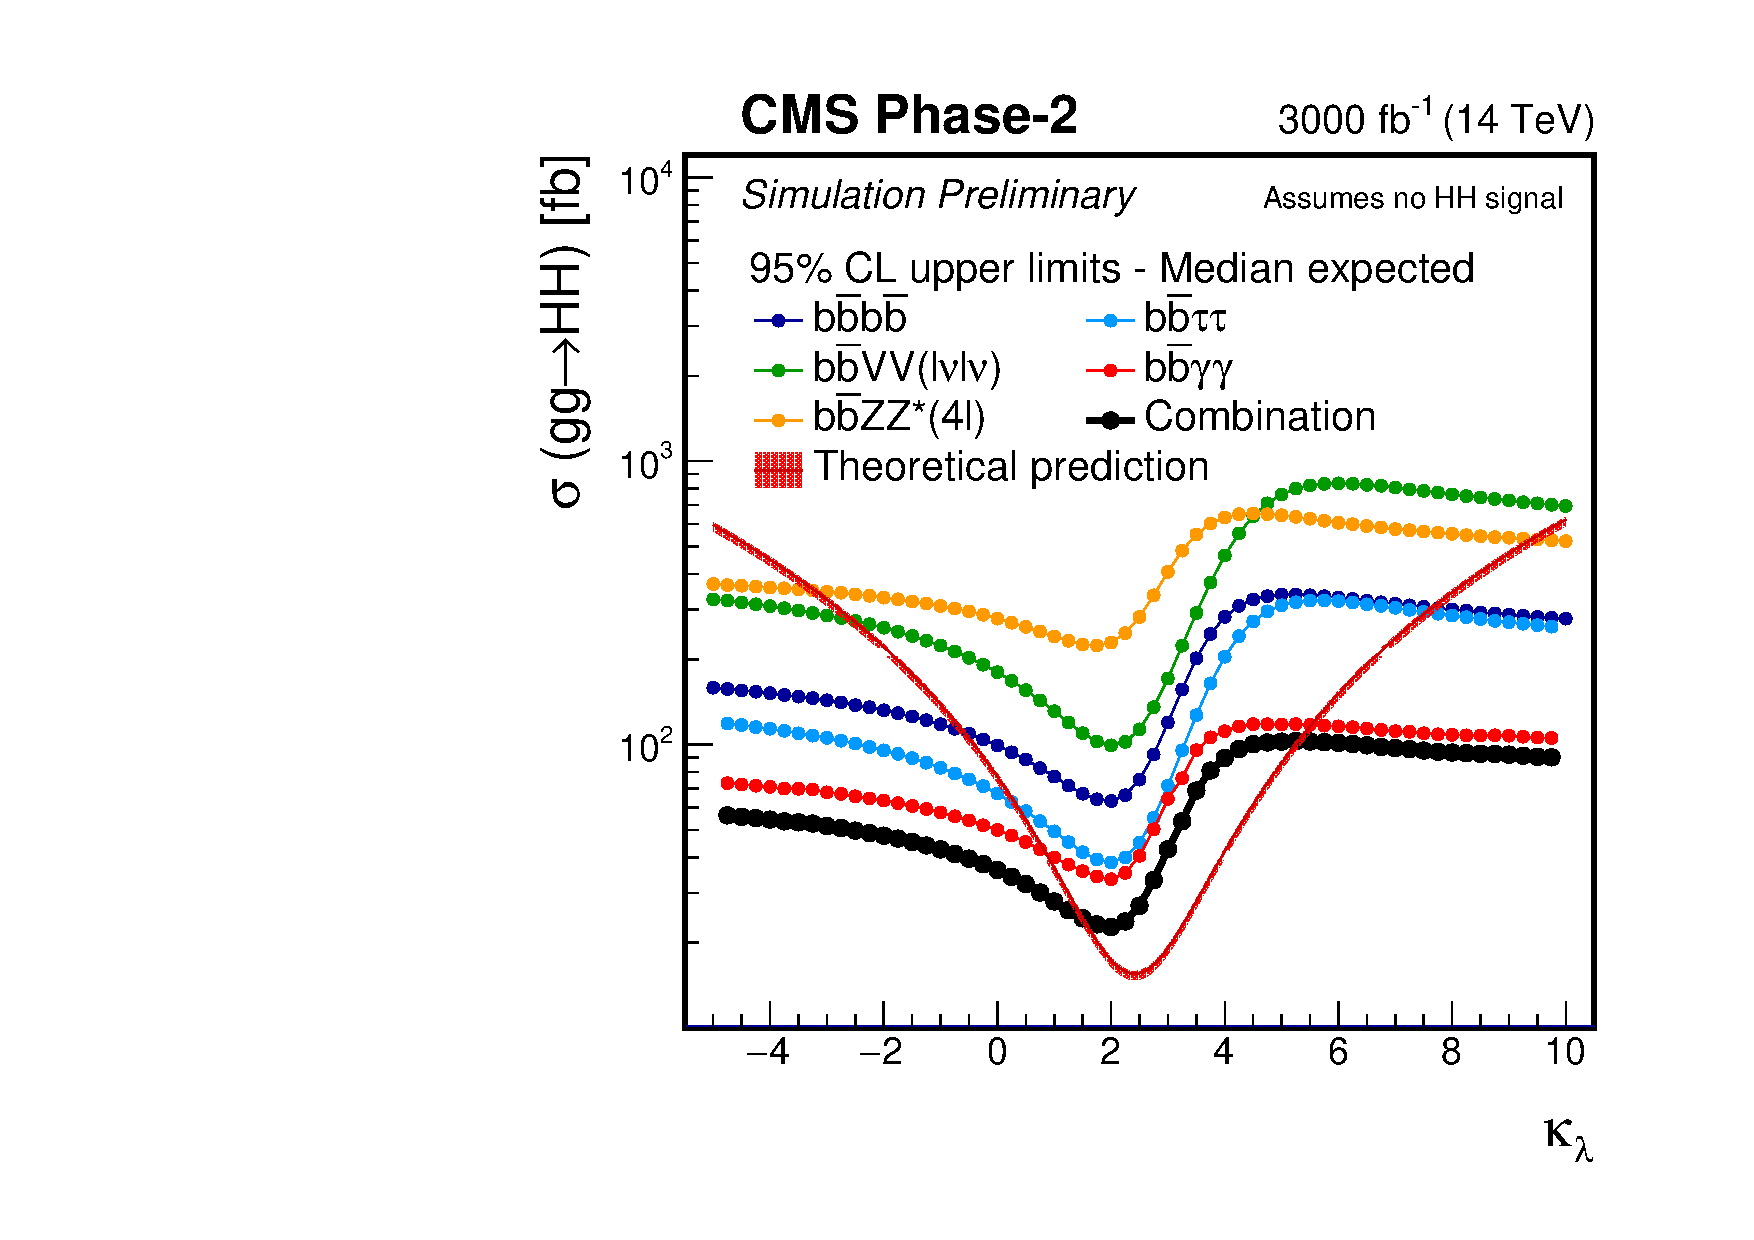
\includegraphics[width=0.6\textwidth]{\main/section3/plots/CMS/limit_comparison.pdf}
%     \caption{Upper limit at the 95\% CL on the \HH production cross section as a function of $\kapl = \lambdahhh/\lambdahhh^\text{SM}$ for the five decays channels investigated and their combination. The red band indicated the theoretical production cross section.}
%     \label{fig:comb:limit_scan}
% \end{figure}

Assuming instead that a \HH signal exists with the properties predicted by the SM, prospects for the measurement of the \lambdahhh are derived.
The scan of the likelihood as a function of the \kapl coupling is shown in Fig.~\ref{sec3:CMSHH:fig:comb_plots}.
The projected confidence interval on this coupling corresponds to $[0.35, 1.9]$ at the 68\% CL and to $[-0.18, 3.6]$ at the 95\% CL.
The peculiar likelihood function structure, characterised by two local minimums, is related to the dependence of the total cross section and \HH kinematic properties on $\kapl$, while the relative height of the two minimums depends to the capability of the analyses to access differential $m_{\HH}$ information.
The degeneracy of the second minimum is largely removed thanks to the $\bbgg$ analysis and its $m_{\HH}$ categorisation.


% \begin{figure}[htbH]
%   \centering
%     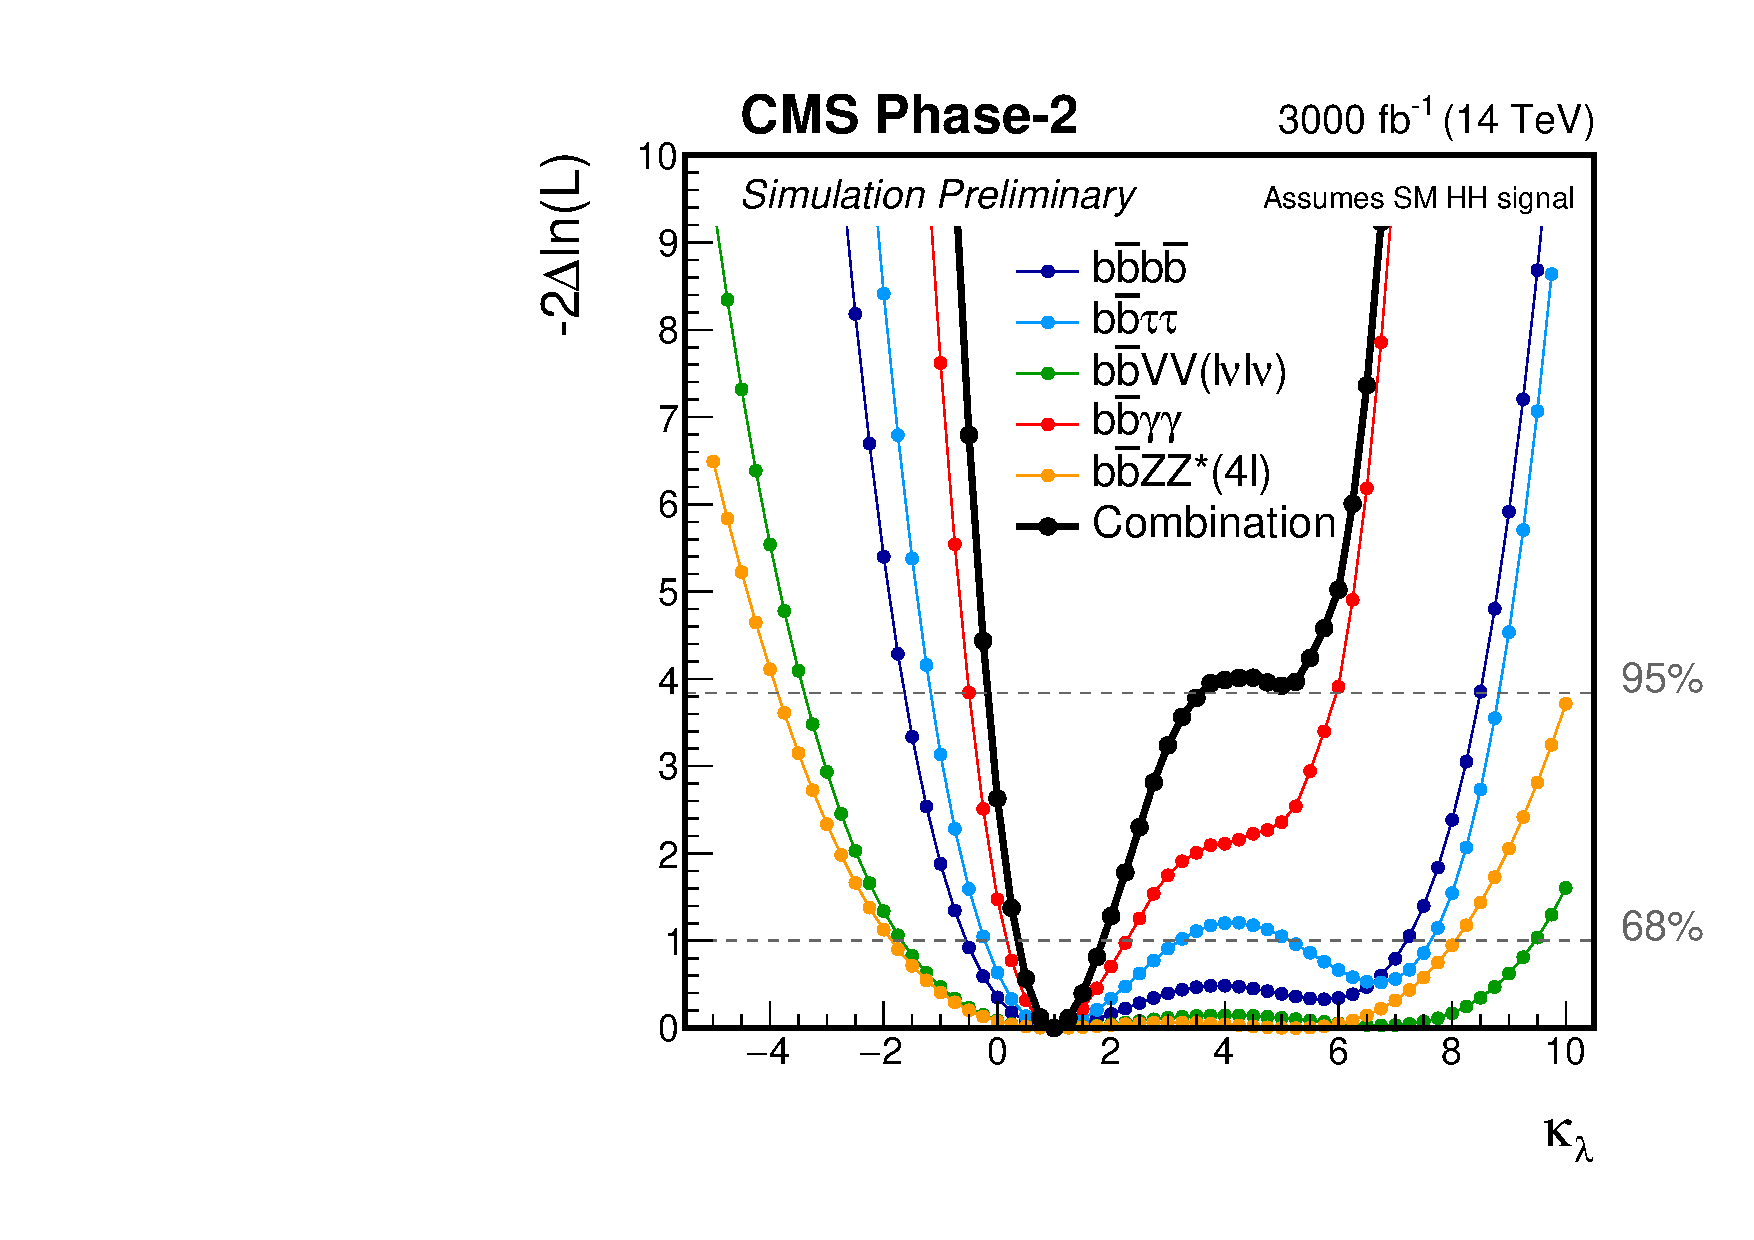
\includegraphics[width=0.6\textwidth]{\main/section3/plots/CMS/likelihood_comparison.pdf}
%     \caption{Expected likelihood scan as a function of $\kappa_\lambda = \lambdahhh/\lambdahhh^\text{SM}$. The functions are shown separately for the five decay channels studied and for their combination.}
%     \label{fig:comb:likelihood_scan}
% \end{figure}

\begin{figure}[htb]
  \centering
   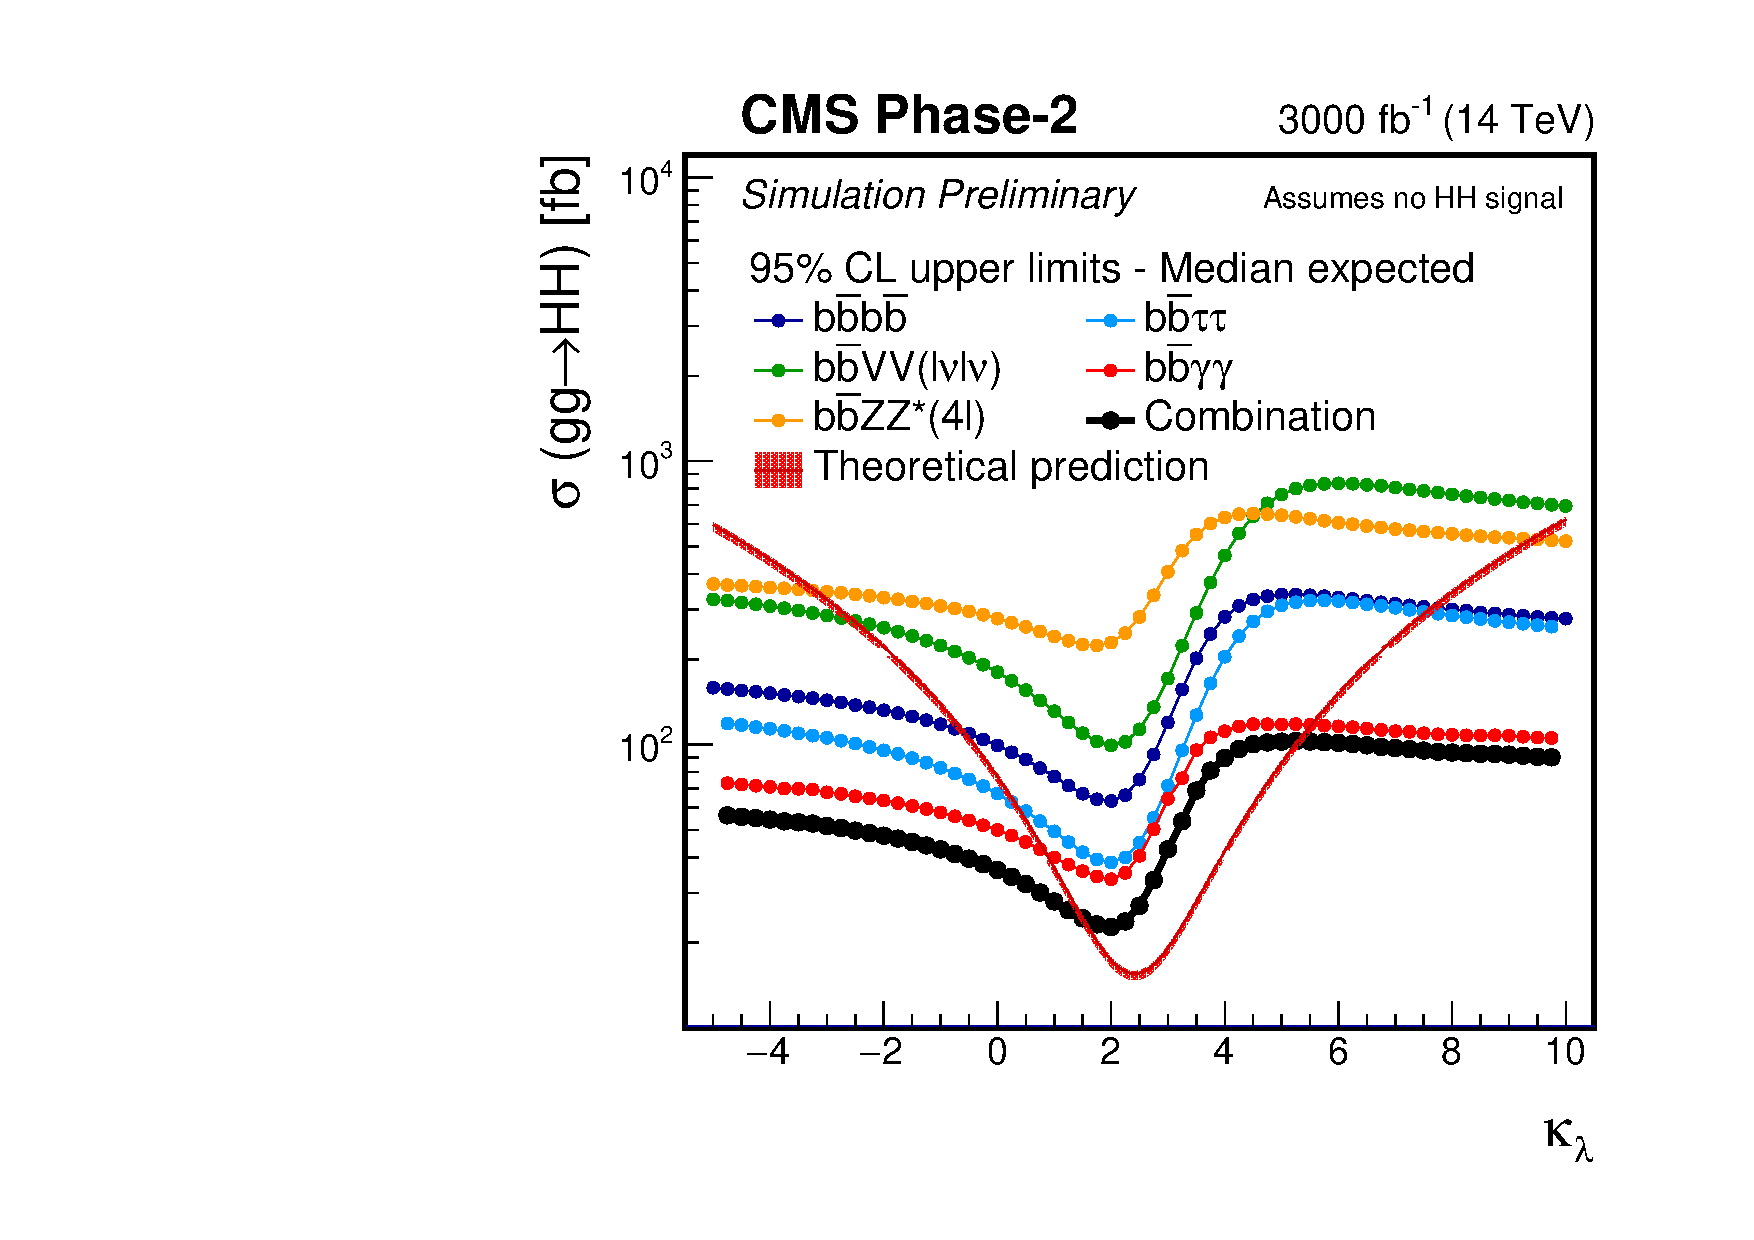
\includegraphics[width=0.48\textwidth]{\main/section3/plots/CMS/limit_comparison.pdf}
    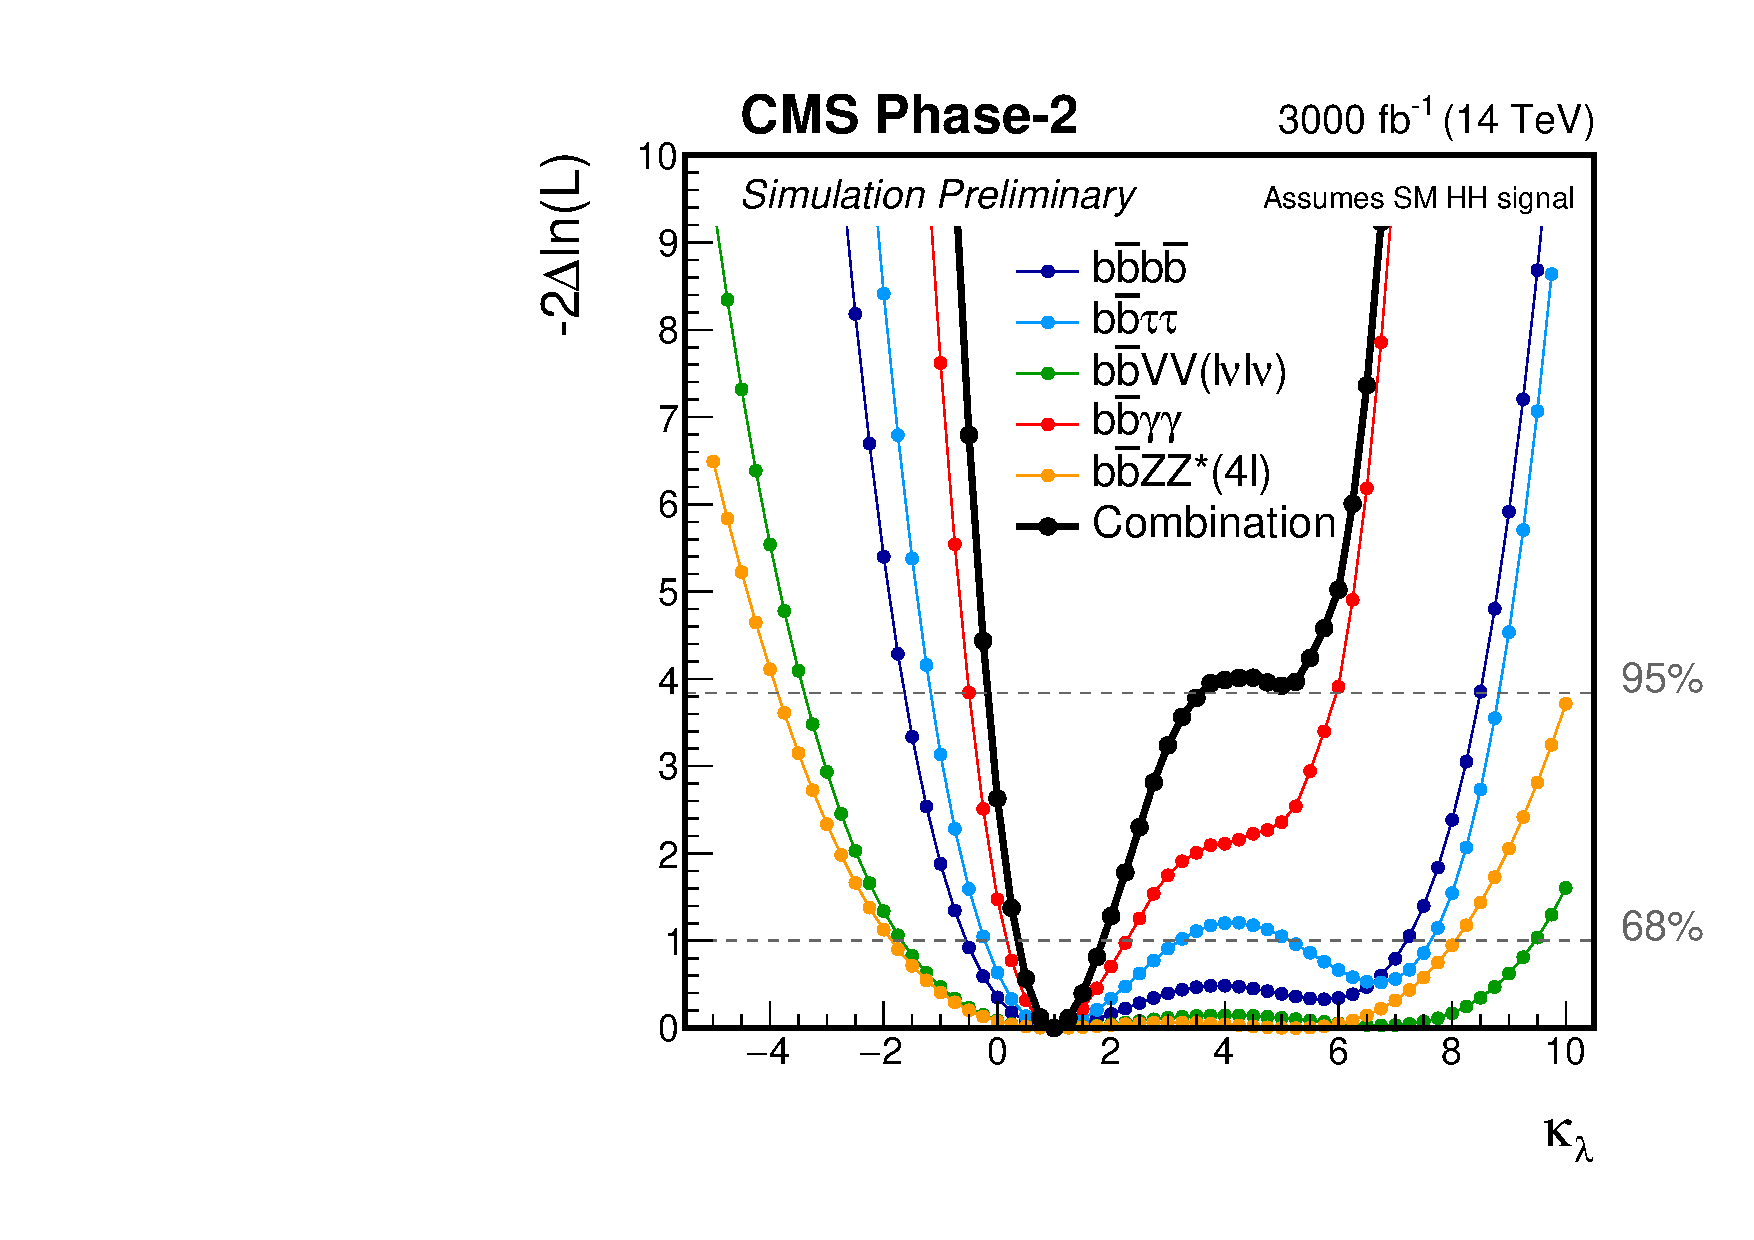
\includegraphics[width=0.48\textwidth]{\main/section3/plots/CMS/likelihood_comparison.pdf}
    \caption{Left: upper limit at the 95\% CL on the \HH production cross section as a function of $\kapl = \lambdahhh/\lambdahhh^\text{SM}$. The red band indicated the theoretical production cross section. Right: expected likelihood scan as a function of $\kappa_\lambda = \lambdahhh/\lambdahhh^\text{SM}$. In both figures the results are shown separately for the five decay channels studied and for their combination.}
    \label{sec3:CMSHH:fig:comb_plots}
\end{figure}


\subsubsection{Combination of measurements}
\label{sec:HH_Combination}

\subfile{\main/section3/HHmeasurement_Combination}

%%%%%%%%%%%%%%%%%%% 
%%%%%%%%%%%%%%%%%%%%%%%%%%%%%%%%%%%%%%%%%%%
\subsection{Double Higgs measurements and trilinear coupling: alternative methods}
\label{sec:HH_meas_th}

%%%%%%%%%%%%%%%%%%% 
%%%%%%%%%%%%%%%%%%%%%%%%%%%%%%%%%%%%%%%%%%%
\subsubsection{Prospects for $hh \to (b \bar b)(WW^*) \to (b \bar b)( \ell^+\ell^- \nu_\ell \bar\nu_\ell)$}
\subfile{\main/section3/bbWW}



%%%%%%%%%%%%%%%%%%% 
%%%%%%%%%%%%%%%%%%%%%%%%%%%%%%%%%%%%%%%%%%%

\subsubsection{Prospects for $bb\gamma\gamma $: Bayesian optimization and BDT}

\subfile{\main/section3/HHbbgammagamma}

%%%%%%%%%%%%%%%%%%% 
%%%%%%%%%%%%%%%%%%%%%%%%%%%%%%%%%%%%%%%%%%%

%%%%%%%%%%%%%%%%%%% 
%%%%%%%%%%%%%%%%%%%%%%%%%%%%%%%%%%%%%%%%%%%


%%%%%%%%%%%%%%%%%%% 
%%%%%%%%%%%%%%%%%%%%%%%%%%%%%%%%%%%%%%%%%%%






\subsection{HE-LHC prospects}
\label{sec:HH_HE}

\subsubsection{Theory studies}
\subfile{\main/section3/HEproj_theory}

\subsubsection{ATLAS studies}
\subfile{\main/section3/HH_HE-LHC_ATLAS}

%%%%%%%%%%%%%%%%%%% 
%%%%%%%%%%%%%%%%%%%%%%%%%%%%%%%%%%%%%%%%%%%


\subsection{Indirect probes}
\label{sec:HH_indirect}

In this section we discuss the possibility of indirectly extract information on the trilinear self interaction of the Higgs boson via precise measurements of single-Higgs production~\cite{McCullough:2013rea,Gorbahn:2016uoy,Degrassi:2016wml,Bizon:2016wgr,DiVita:2017eyz,Barklow:2017awn,Maltoni:2017ims,DiVita:2017vrr,Maltoni:2018ttu} at the HL-LHC and HE-LHC. This strategy is complementary to the direct measurement via double-Higgs production, which already at leading order,~i.e.~at one loop in the case of $gg \to HH$, depends on the trilinear Higgs self interaction. In the case of single-Higgs production, on the contrary, the Higgs self interactions enter only via one-loop corrections, i.e., at the two-loop level for the gluon-fusion ($ggF$) production mode. The effects of modified Higgs self interactions are therefore generically much smaller, but for single-Higgs production processes the precision of the experimental measurements is and will be much better than for double-Higgs production. This, and the fact that for single-Higgs production many different final states and both inclusive as well as  differential measurements are possible will lead to competitive indirect determinations of the trilinear Higgs self coupling. In \cite{Degrassi:2017ucl,Kribs:2017znd} also electroweak precision observables have been considered to this purpose.

\subsubsection{Indirect probes through single Higgs boson production}

\subfile{\main/section3/HL-HE-tril_indirect_computation}

\subsubsection{Indirect probes of the trilinear coupling through differential distributions measurements}

\subfile{\main/section3/HL_CMS_FTR_18_020}


\subsubsection{Global fit}
\label{sec:HH_Global_fit}
\subfile{\main/section3/HL-HE-tril_indirect_globalfit}

\subsection{Implications of the HH measurements}
\label{sec:HH_implications}

\subsubsection{Implications for flavor models}
\begin{center}
\textit{by Martin Bauer, Marcela Carena and Adri\'an Carmona}
\end{center}

In the Two-Higgs-Doublet Model (2HDM), the term $H_1 H_2\equiv H_1^T (i\sigma_2) H_2 $ is a SM singlet which can however be charged under an additional $U(1)$ flavor symmetry. This is an interesting possibility that allows to generate the different fermion masses with a Froggatt-Nielsen (FN) mechanism where the flavon is replaced by the $H_1 H_2$ operator. In this way, the new physics scale $\Lambda$ where the higher dimensional FN operators are generated is tied to the electroweak scale, leading to much stronger phenomenological consequences. Let us assume for concreteness a type-I like 2DHM with the following Yukawa Lagrangian 
\begin{align}
\label{eq:yuk1}
\mathcal{L}_Y&\supset  y^u_{ij} \left(\frac{H_1 H_2}{\Lambda^2}\right)^{n_{u_{ij}}}\bar{q}_L^{i}H_1 u_{R}^j+y^d_{ij} \left(\frac{H_1^{\dagger} H_2^{\dagger}}{\Lambda^2}\right)^{n_{d_{ij}}}\bar{q}_L^{i}\tilde{H}_1 d_{R}^j+y_{ij}^{\ell}\left(\frac{H_1^{\dagger}H_2^{\dagger}}{\Lambda^2}\right)^{n_{e_{ij}}}\bar{\ell}_{L}^i\tilde{H}_1 e_R^j
+\mathrm{h.c.}\,,
\end{align}
where $\tilde{H}_1\equiv i\sigma_2 H^{\ast}_1$ as usual and the charges $n_{u,d,e}$ are a combination of the $U(1)$ charges of $H_1$, $(H_1H_2)$ and the different SM fermion fields. For simplicity, we set the flavor charges of $(H_1 H_2)$ and $H_2$ to $0$ and $1$, respectively, such that  
\begin{align}
n_{u_{ij}}=a_{q_i}-a_{u_j},\quad n_{d_{ij}}=-a_{q_i}+a_{d_j},\quad n_{e_{ij}}=-a_{\ell_i}+a_{e_j},
\end{align}
if we denote by $a_{q_i},a_{u_i}, \ldots,$ the $U(1)$ charges of the SM fermions. In general, the fermion masses are given by
\begin{align}\label{eq:epsilon}
m_\psi=y_{\psi} \varepsilon^{n_\psi} \frac{v}{\sqrt{2}}, \quad \varepsilon = \frac{v_1 v_2}{2\Lambda^2}=\frac{t_\beta}{1+t_\beta^2}\frac{v^2}{2\Lambda^2},
\end{align}
with the vacuum expectation values $\langle H_{1, 2}\rangle=v_{1, 2}$ and $t_\beta \equiv v_1/v_2$. Besides being able to accommodate the observed hierarchy of SM fermion masses and mixing angles for the right assignment of flavor charges \cite{Bauer:2015fxa, Bauer:2015kzy}, this framework can lead to enhanced diagonal Yukawa couplings between the Higgs and the SM fermions while having suppressed flavour changing neutral currents (FCNCs). If we denote by $h$ and $H$ the two neutral scalar mass eigen-states, with $h$ being the observed $125$ \UGeV Higgs, the couplings between the scalars $\varphi=h,H$ and SM fermions $\psi_{L_i, R_i}= P_{L,R} \psi_i$ in the mass eigen-basis read 
\begin{equation}\label{eq:newlagrangian}
\mathcal{L}= g_{\varphi \psi_{L_i} \psi_{R_j} }\, \varphi \,\bar \psi_{L_i} \psi_{R_j}+\mathrm{h.c.}
\end{equation}
with $i$, such that $u_i=u, c,t$,\,  $d_i=d,s,b$ and $e_i=e,\mu,\tau$. This induces 
flavor-diagonal couplings 
\begin{align}\label{eq:diagocoup}
g_{\varphi \psi_{L_i}\psi_{R_i}}= \kappa^\varphi_{\psi_i}\, \frac{m_{\psi_i}}{v} =\left(g^{\varphi}_{\psi_i}(\alpha,\beta)+n_{\psi_i}\, f^\varphi(\alpha, \beta)\right)\frac{m_{\psi_i}}{v},
\end{align}
as well as flavor off-diagonal couplings
 \begin{align}\label{eq:foffc}
g_{\varphi \psi_{L_i}\psi_{R_j}}&=  f^\varphi(\alpha, \beta)\left(\mathcal{A}_{ij}\frac{m_{\psi_j}}{v}-\frac{m_{\psi_i}}{v}\mathcal{B}_{ij} \right)\,.
\end{align}
The flavor universal functions in \eqref{eq:diagocoup} and \eqref{eq:foffc} read
\begin{align}
g^h_{\psi_i}=\frac{c_{\beta-\alpha}}{t_\beta}+s_{\beta-\alpha}\,,\qquad g^H_{\psi_i}=c_{\beta-\alpha}-\frac{s_{\beta-\alpha}}{t_\beta}\,,
\end{align}
and
\begin{align}\label{eq:fFs}
f^h(\alpha,\beta)&=c_{\beta-\alpha}\Big(\frac{1}{t_\beta}-t_\beta\Big)+2s_{\beta-\alpha}\,,\quad f^H(\alpha,\beta)=-s_{\beta-\alpha}\Big(\frac{1}{t_\beta}-t_\beta\Big)+2c_{\beta-\alpha}\,,
\end{align}
where $c_{x}\equiv \cos x$, $s_x\equiv \sin x$. One can see that, unless all flavor charges for a given type of fermions are equal, the off-diagonal elements in matrices $\mathcal{A}$ and $\mathcal{B}$ lead to FCNCs which are chirally suppressed by powers of the ratio~$\varepsilon$, see \cite{Bauer:2017cov} for more details.

The scalar couplings to the different gauge bosons are the same as in a normal type-I 2HDM while the scalar coupling between the heavy Higgs $H$ and two SM Higgs scalars $h$, as well as the triple Higgs coupling can be expressed as \cite{Boudjema:2001ii, Gunion:2002zf}
\begin{align}
\label{eq:mainn1}
g_{Hhh}&=\frac{c_{\beta-\alpha}}{v}\!\left[\big(1\!-\!f^h(\alpha,\beta)s_{\beta-\alpha}\big)\big(3M_A^2\!-\!2m_h^2\!-\!M_H^2\big)\!-\!M_A^2\right],\\
g_{hhh}&= -\frac{3}{v}\!\left[f^h(\alpha,\beta)c_{\beta-\alpha}^2(m_h^2-M_A^2)+m_h^2s_{\beta-\alpha}\right],\label{eq:mainn2}
\end{align}
where $M_A$ is the pseudoscalar mass. The $U(1)$ flavor symmetry restricts the number of allowed terms in the scalar potential forbidding e.g. terms proportional to $H_1 H_2$. The interesting feature is that one can rewrite such self scalar interactions with the help of the function $f^h(\alpha,\beta)$, since it is somehow related to the combination $H_1 H_2^{\dagger}$ appearing in both the scalar potential and the higher dimensional operators generating the different Yukawa couplings. Therefore, the parameter space for which $f^h(\alpha,\beta)\gg 1$ and  $c_{\beta-\alpha}\neq 0$ leads to maximally enhanced diagonal couplings of the SM Higgs to fermions \eqref{eq:diagocoup} as well as to an enhancement of the trilinear couplings \eqref{eq:mainn1} and \eqref{eq:mainn2}. For maximally enhanced Yukawa couplings, the mass of the heavy Higgs $H$ cannot be taken arbitrarily large and resonant Higgs pair production has to be present. This correlation between the enhancement of the Higgs Yukawa couplings $\kappa^h_{\psi}$ and $\text{Br}(H \to hh)$ is illustrated for $M_H=M_A=M_{H^\pm}=500$ \UGeV in Fig. \ref{fig:BRvskappa} where we plot the dependence of $\text{Br}(H \to hh)$ on $c_{\beta-\alpha} $ and $ t_\beta$.  The dashed contours correspond to constant values of $|\kappa_{\psi}^h|$ for $n_{\psi}=1$. This correlation does not dependent of the factor $n_\psi$, although  $n_\psi > 1$ leads to a larger enhancement. The two exceptions for which this correlation breaks down are the limits $c_{\beta-\alpha}\approx 0$ and $c_{\beta-\alpha}\approx \pm 1$. Whereas the second case is strongly disfavoured by SM Higgs couplings strength measurements, the first one (which corresponds to the decoupling limit) is at odds with the flavor model, for it requires large values of the spurion $\mu_3\propto M_A$ which softly breaks the $U(1)$ flavor symmetry. 




%
 \begin{figure}
 \begin{center}
 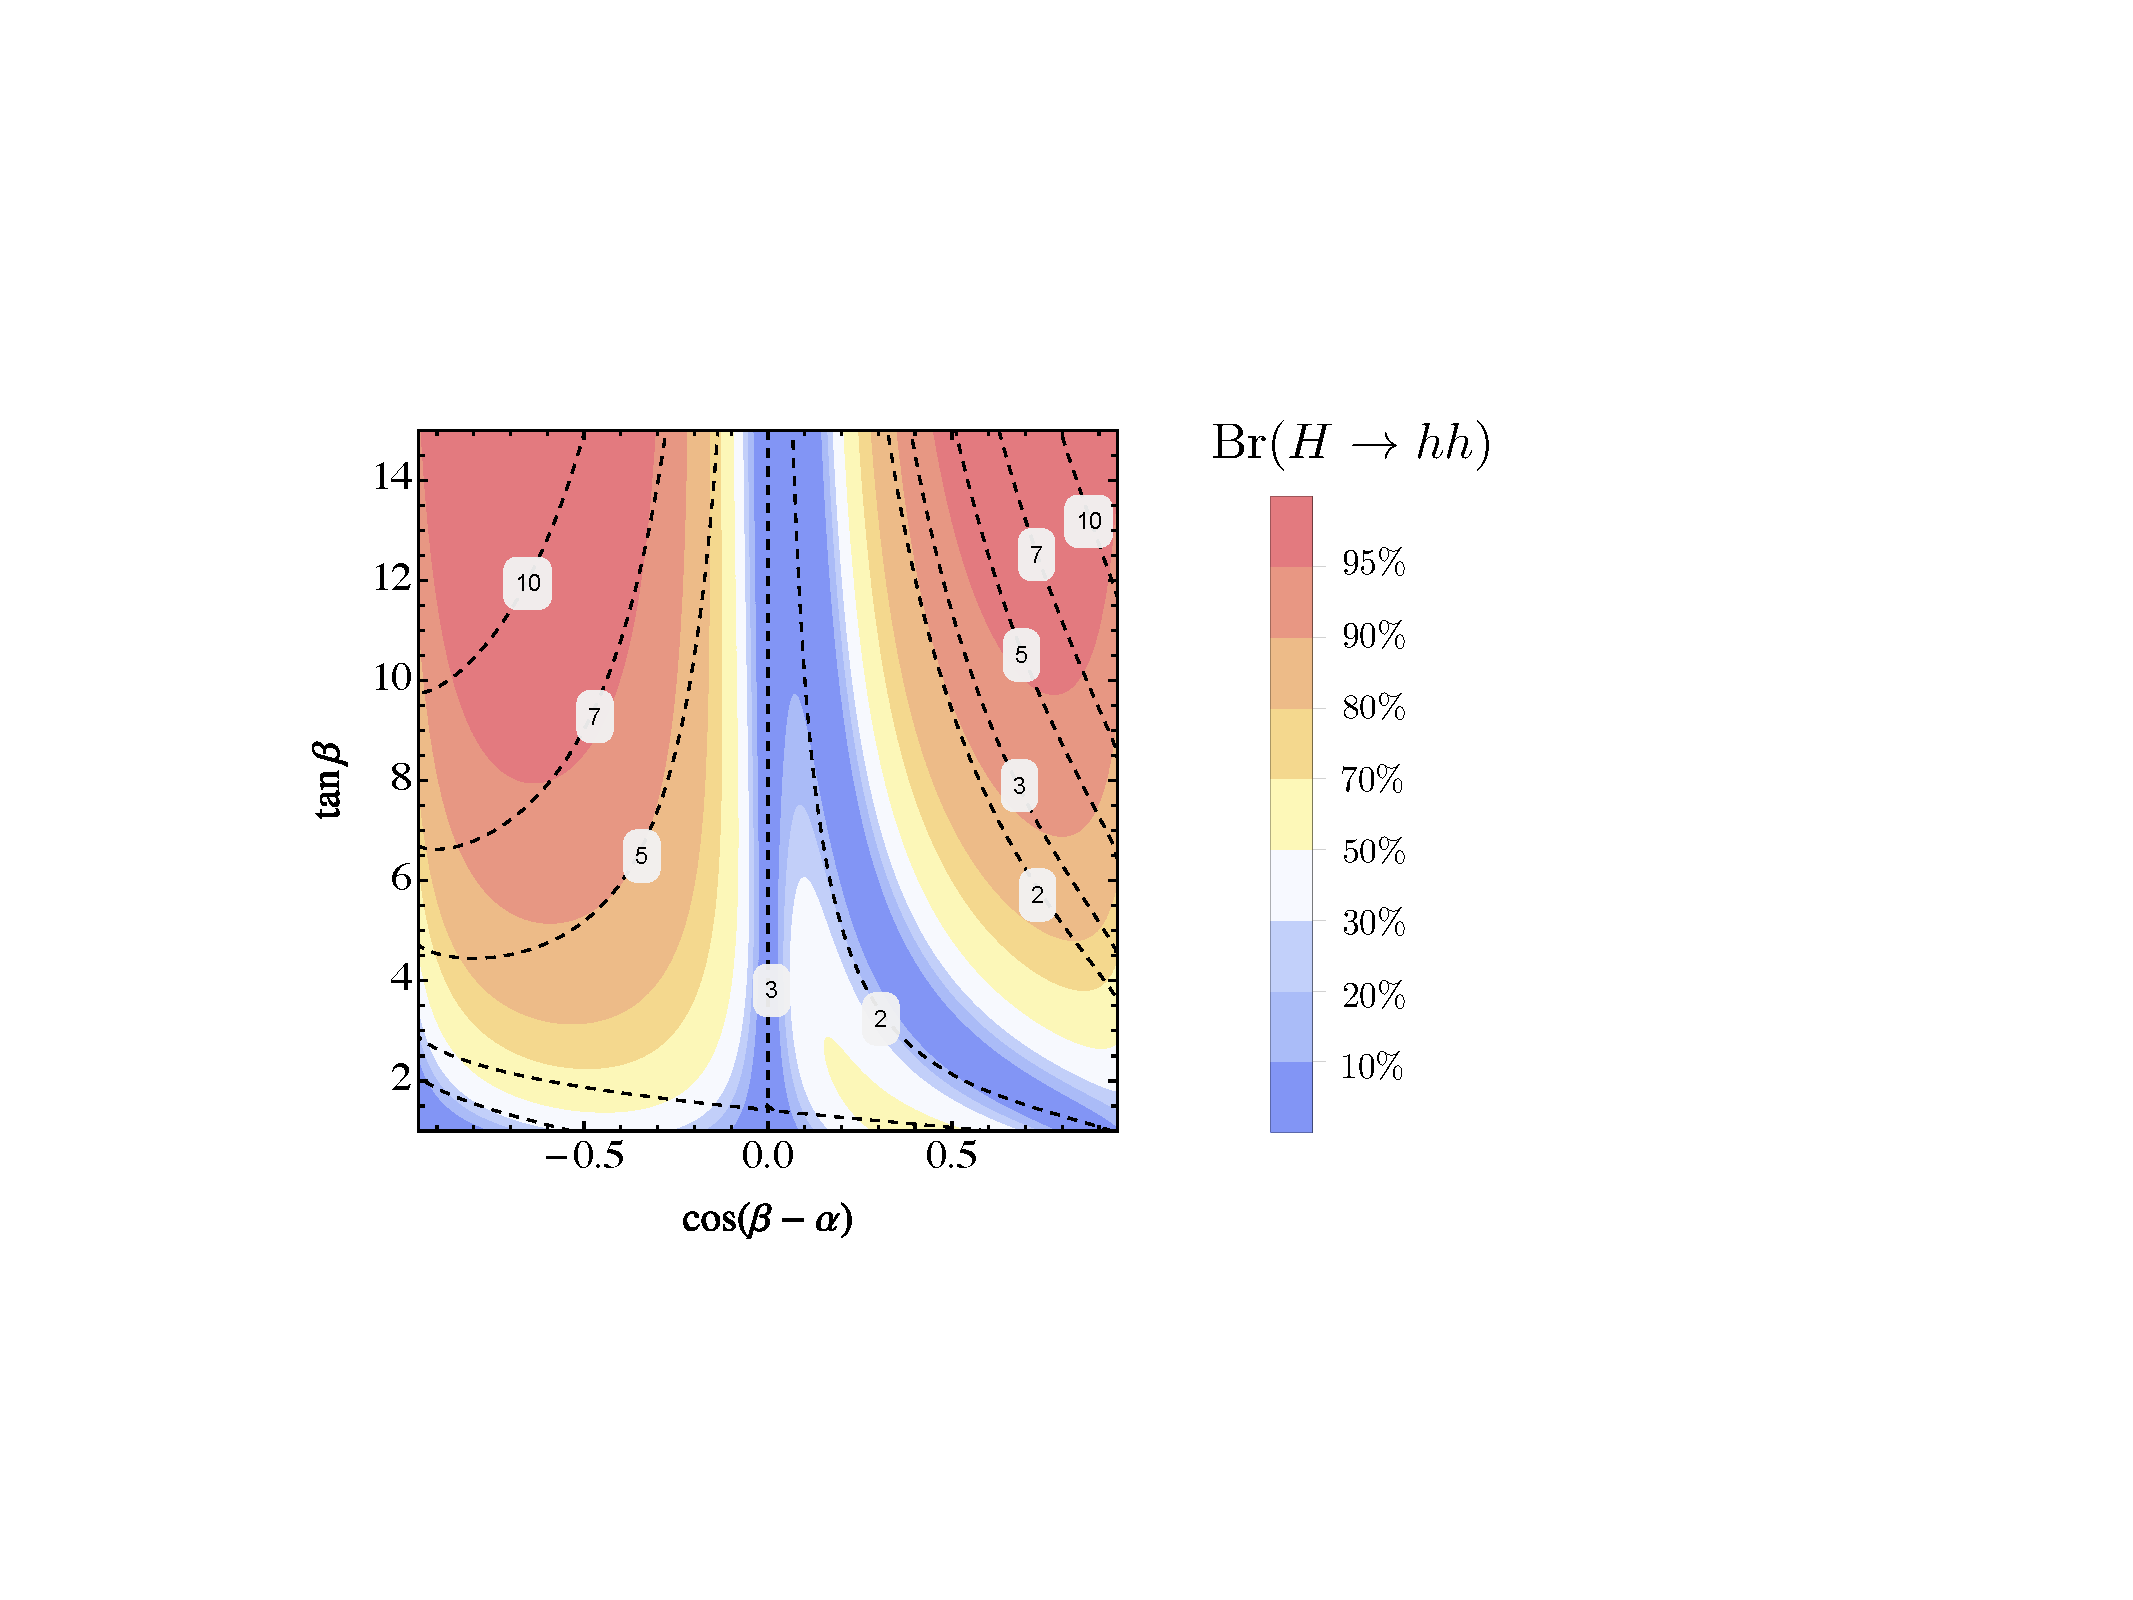
\includegraphics[width=.8\textwidth]{\main/section3/plots/BRvskap.pdf}
 \caption{\label{fig:BRvskappa} $\text{Br}(H \to hh)$ as a function of $\cos(\beta-\alpha)$ and $ \tan\beta$ for $M_H=M_{H^\pm}=550$ \UGeV and $M_A=450$ \UGeV. The dashed contours correspond to constant values $|\kappa_{\psi}^h|$ for $n_{\psi}=1$.}
 \end{center}
  \vspace{-.6cm}
 \end{figure}
%
%
\begin{figure*}
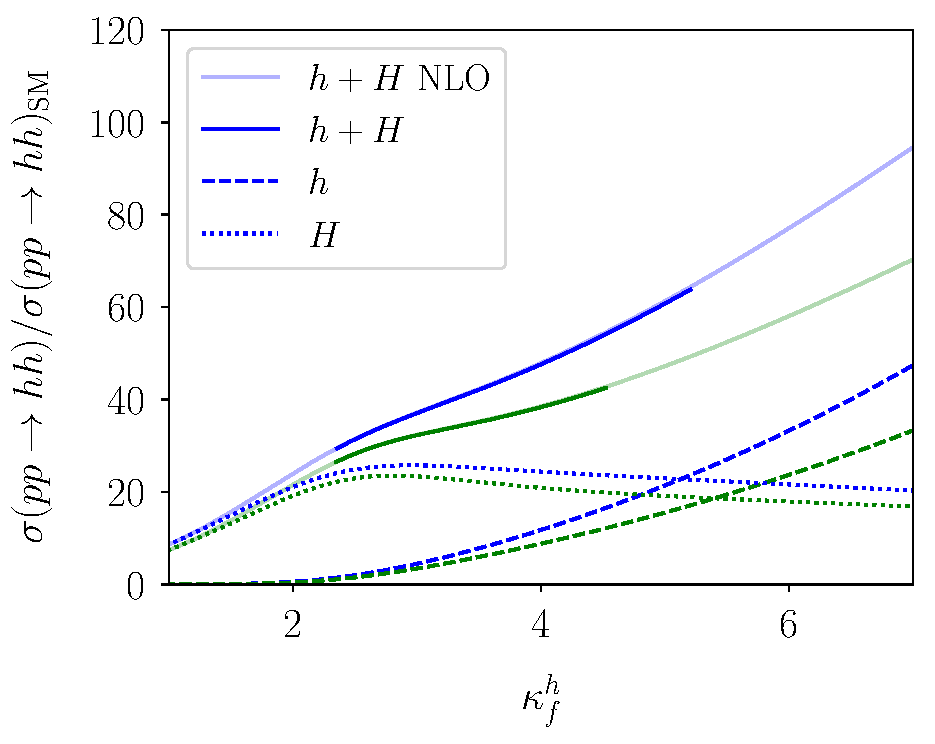
\includegraphics[width=.465\textwidth]{\main/section3/plots/xsec_3.pdf}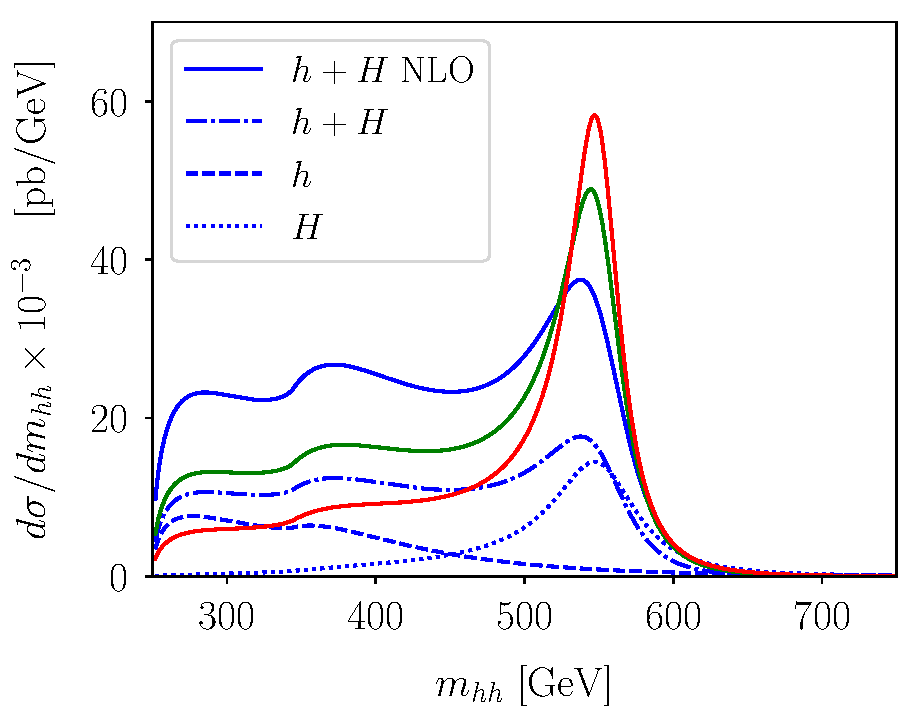
\includegraphics[width=.49\textwidth]{\main/section3/plots/diff.pdf}
	\caption{\label{fig:xsecc} Left: Cross section for Higgs pair production in units of the SM prediction as a function of $\kappa_{\psi}^h$ for $c_{\beta-\alpha}=-0.45~(-0.4)$ and $M_A=450$ \UGeV , $M_H=M_{H^\pm}=550$ \UGeV in blue (green) at $\sqrt{s}=27 $ \UTeV. Right: Invariant mass distribution for the different contributions to the signal with $c_{\beta-\alpha}=-0.45$ and $\kappa^h_{\psi}=5$ (blue),  $\kappa_{\psi}^h=4$ (green) and $\kappa_{\psi}^h=3$ (red) at $\sqrt{s}=27 $ \UTeV, respectively.} 
	\label{fig:hhflavourxsanddistr}
\end{figure*}
%

The enhancement in $\text{Br}(H\to hh)$ shown in Figure~\ref{fig:BRvskappa} is partially cancelled in the production cross section $\sigma(gg\to H)$ for large values of $t_{\beta}$ due to the fact that $\sigma(gg\to H)\propto 1+1/t_\beta^2-(\kappa_t^h)^2$, with $\kappa_t^h \approx 1$. However, the cross-section $\sigma(gg\to h\to hh)$ is not suppressed for such values of $t_{\beta}$ and the combination of both contributions leads to a continuous enhancement in the di-Higgs cross-section. There is therefore a non-trivial interplay between resonant and non-resonant contributions, which we illustrate in the left panel of Fig.~\ref{fig:xsecc}, where we plot both contributions assuming as a function of $\kappa_{\psi}^h$ for fixed values of $c_{\beta-\alpha}$ (which is a monotonic function of $t_{\beta}$). We assume a centre-of-mass energy of $\sqrt{s}=27$ \UTeV and set $M_A=450$ \UGeV and $M_{H}=M_{H^{\pm}}=550$ \UGeV, while choosing two different values of $c_{\beta-\alpha}=-0.45$ and $-0.4$. Dashed (dotted) lines correspond to the non-resonant (resonant) contributions, whereas the solid lines represent the full $\sigma(gg\to hh)$ in the 2HDM in units of the SM prediction, both at LO and NLO.   Solid lines show the NLO results, while the solid shaded lines mark the values of $\kappa_{\psi}$ excluded by perturbativity and unitarity constraints~\cite{Eriksson:2009ws}.  More details about the calculation of the signal and plots for $\sqrt{s}=13$ \UTeV can be found in Ref.~\cite{Bauer:2017cov}.  The values of $\kappa_{\psi}^h$ in Fig.~\ref{fig:xsecc} correspond to $n_{\psi}=1$ but values of $\mathcal{O}(10)$ and larger are obtained for $n_{\psi}>1$. We also show in the right panel of Fig.~\ref{fig:xsecc} the invariant mass distribution for the different contributions to the di-Higgs signal for $c_{\beta-\alpha}=-0.45$ and three different values of $\kappa_{\psi}^{h}=3, 4$ and $5$. The interesting feature is that, when the enhancement in the Higgs Yukawa couplings is large enough, the interference between both non-resonant and resonant contributions turns the broad peak into a shoulder in the $d\sigma/ dm_{hh}$ distribution for the total cross section, as shown for the case $\kappa_{\psi}^h=5$ by the blue line in the right panel of Fig.~\ref{fig:xsecc}. Resolving such shape in the  invariant mass distribution can be quite challenging. We encourage a dedicated analysis considering the corresponding $d\sigma/dm_{hh}$ templates to maximise the sensitivity to features in the di-Higgs invariant mass distribution from the simultaneous enhancement of  $g_{hhh}$, $g_{Hhh}$ and $\kappa^h_{\psi}$.\\




\subsubsection{Implications for theories of electroweak phase transition}
\begin{center}
\textit{by Jonathan Kozaczuk, Andrew J. Long, Jose Miguel No, and Michael J. Ramsey-Musolf}
\end{center}

\noindent{\it Introduction.} Explaining the origin of the cosmic matter-antimatter asymmetry is a key open problem at the interface of high energy physics and cosmology. A number of scenarios have been proposed, ranging in energy scales from $\sim 10^{12}$ and above to below the electroweak scale and corresponding to different eras in cosmic history. One of the most compelling -- electroweak baryogenesis --  ties the generation of the asymmetry to electroweak symmetry breaking (for a review, see Ref.~\cite{Morrissey:2012db}). In this scenario, the universe must have undergone a first order phase from the electroweak symmetric to broken phase at a temperature $T_\mathrm{EW} \sim 100$ \UGeV. If such a transition occurred, then there must have also existed sufficiently active CP-violating interactions to produce the observed asymmetry. Neither requirement is satisfied by the Standard Model. The symmetry-breaking transition for a 125 \UGeV Higgs boson is known to be of a crossover type, and the CP-violating interactions encoded in the Cabibbo-Kobayashi-Maskawa matrix are too feeble to have produced the observed asymmetry. Thus, viable electroweak baryogenesis (EWBG) requires physics beyond the standard model that couples to the Higgs boson.

The HE LHC would provide new opportunities to search for this BSM physics. Studies of di-Higgs production, measurements of the Higgs triple self-coupling, and precision tests of other Higgs couplings are particularly interesting as probes of the new interactions needed for a first order electroweak phase transition (EWPT). For the first order phase transition to be sufficiently strong, so as to provide the needed conditions for EWBG, the new interactions must be mediated by particles with masses below roughly one \UTeV, making them accessible to $pp$ collisions at $\sqrt{s} = 27$ \UTeV. While a definitive program of searching for these interactions would likely require higher centre of mass energy, the HE LHC would significantly extend the discovery reach over what is accessible at the HL LHC. Below, we provide a few key examples that illustrate this possibility.

\noindent{\it Higgs Potential at Finite Temperature.} The nature of the EWSB transition is governed by the temperature-dependent Higgs potential, $V_\mathrm{EFF}(\varphi, T)$. In the regime where $T\gg M_W$, this potential takes the 
simple form
\begin{equation}
V_\mathrm{EFF}(\varphi,T) = D(T^2-T_0^2)\varphi^2 -(ET+e)\varphi^3 + {\bar\lambda}\varphi^4+\cdots ~~.
\label{eq:HiggspotT}
\end{equation}
In the SM one has $e=0$, while $D$, $T_0$, $E$ and ${\bar\lambda}$ are all non-vanishing functions of the zero temperature parameters of the theory (e.g., gauge, Yukawa, and Higgs self-couplings). At any temperature, the minimum of energy is obtained when $\varphi$ equals its vacuum expectation value $v(T)$, with $v(0) = 246$ \UGeV. The Higgs boson field is just the difference $h=\varphi-v(0)$. 

At sufficiently high temperatures, the minimum of the potential resides at the origin, {\it i.e.}, $v(T) = 0$. As the universe cools, however, the minimum eventually moves away from the origin, corresponding to the onset of EWSB. The details of this evolution, and the nature of the transition (first order, second order, or crossover) depends on the values of the couplings in Eq.~(\ref{eq:HiggspotT}). Since the latter are determined by the $T=0$ interactions, measurements of Higgs boson properties allow one to infer the thermal history of electroweak symmetry breaking. 

Assuming the SM form of the $T=0$ Higgs potential and Higgs couplings to other SM particles, lattice studies imply that for a 125 \UGeV Higgs boson, the symmetry-breaking transition is of a cross over type\cite{Rummukainen:1998as,Csikor:1998eu,Laine:1998jb,Gurtler:1997hr}. Thus, one of the three \lq\lq Sakharov conditions" for successful baryogenesis\cite{Sakharov:1967dj} -- out of equilibrium dynamics -- would not have been satisfied, thereby precluding EWBG. However, the presence of additional bosons that interact with the Higgs boson could yield a first order EWPT even for a 125 \UGeV Higgs boson (see e.g., \cite{Morrissey:2012db,Assamagan:2016azc}). A sufficiently strong first order EWPT may arise if these interactions induce changes in the zero-temperature vacuum structure of the scalar potential and/or generate finite-temperature quantum corrections that modify the parameters in Eq.~(\eqref{eq:HiggspotT}). In addition, the presence new neutral scalars that may also obtain vacuum expectation values may allow for a richer thermal history than in the SM universe, including the presence of new symmetry-breaking phases that preceded the presence of the \lq\lq Higgs phase"\cite{Patel:2012pi,Patel:2013zla,Blinov:2015sna}. 

\noindent{\it Collider Probes.} Existing searches for new scalars at the LHC, together with present measurements of Higgs boson properties, generally rule out a strong first order transition if the new scalars are charged under S(3$)_C$\cite{Katz:2014bha,Katz:2015uja}. In contrast, interactions involving scalars that carry only EW quantum numbers (EW multiplets) or no SM quantum numbers at all (singlets) are considerably less constrained. Cross sections for directly producing these scalars can be as small as a few fb when model parameters are consistent with a strong first order EWPT. If one of these scenarios is realised in nature, then one may or may not be able to discover it at the HL LHC. The higher energy and integrated luminosity of the HE LHC would significantly expand this discovery potential. 

Perhaps, the simplest illustration of this potential is the extension of the SM scalar sector with a single real singlet scalar\cite{Espinosa:1993bs,Choi:1993cv,Ham:2004cf,Profumo:2007wc,Cline:2012hg,Espinosa:2011ax,No:2013wsa,Curtin:2014jma,Kotwal:2016tex,Brauner:2016fla,Huang:2016cjm,Chen:2017qcz,Huang:2017jws}, the \lq\lq xSM" \cite{Barger:2007im} (for analogous studies with a complex singlet, see \cite{Jiang:2015cwa,Chiang:2017nmu}). 
%Singlet scalars occur copiously in extensions of the SM, but examination of the additional degrees of freedom and interactions is not essential for identifying the EWPT dynamics. 
The xSM contains two Higgs-like scalars, $\rm h_{1}$ and $\rm h_{2}$ that are admixtures of the neutral component of the SM Higgs doublet and the singlet. For a wide range or model parameters, the interactions in the xSM scalar potential can  lead to a strong first order EWPT when the SM-like state $\rm h_1$ has a mass of 125 \UGeV. The associated collider signatures direct and indirect effects:  direct production of scalar pairs; include modifications of the Higgs self-coupling, which may be as as large as $\mathcal{O}(1)$ or small as a few percent; and a shift in the associated production ($\rm Zh_1$) cross section. 

%two SM-like scalars $h_1$ through an on-shell $h_2$. 
We consider first scalar pair production. In pp collisions, a pair of SM-like scalars $\rm h_1$ can be produced through an on-shell $\rm h_2$, corresponding to the so-called \lq\lq resonant di-Higgs production".  Each $\rm h_1$ then decays to the conventional Higgs boson decay products, yielding various combinations. The possibilities for discovery through the  \lq\lq resonant di-Higgs production" process are illustrated in Fig.~\ref{fig:ewpt_resdihiggs}, where the results are obtained by combining the 4\texttau\ and b\={b}\textgamma\textgamma\ final states\cite{Kotwal:2016tex} (for early studies of resonant di-Higgs production, see, {\it e.g.}. Ref.~\cite{Baur:2003gp}). Each coloured band gives the projected significance $N_\sigma$ of observation as a function of the $\rm h_2$ mass, with the $N_\sigma$ range obtained by varying over all other model parameters consistent with a strong first order EWPT, constraints from EW precision observables, and present LHC Higgs signal strength determinations.  The maximum $\rm h_2$ mass consistent with a strong first order EWPT is just below 900~\UGeV.  Results are shown for different prospective centre of mass energies.

At the time this work was completed, no analysis had been performed for $\sqrt{s} = 27 $ \UTeV and 15 ab$^{-1}$ integrated luminosity. Consequently, we show in the left panel the reach for the LHC and a 100 \UTeV $pp$ collider and in the right panel the corresponding reach for $\sqrt{s} = 50$, 100, and 200 \UTeV with 30 ab$^{-1}$. As one can see, the HL-LHC discovery potential is limited to a relatively modest portion of the light $\rm h_2$ parameter space, whereas the FCC-hh with 30~ab$^{-1}$ would enable discovery over the entire first order EWPT-viable parameter space in this model. Interpolating by eye, one can anticipate that the reach for the HE LHC will lie somewhere between that of the LHC and the 50 \UTeV band in the right panel. 

\begin{figure}[hbtp]
  \begin{center}
    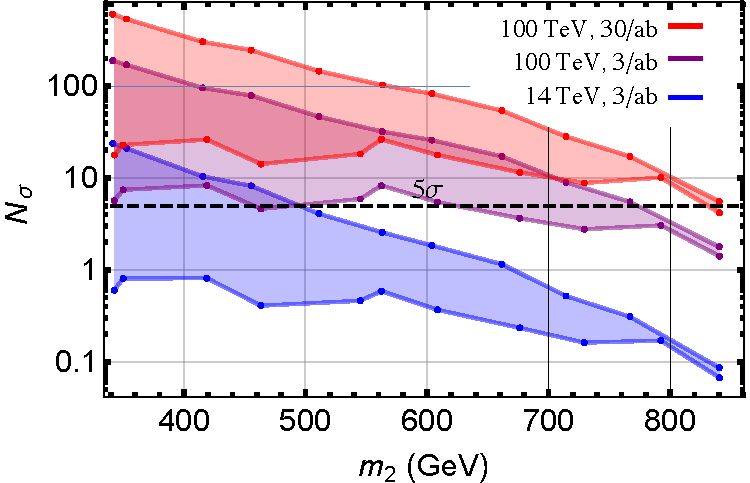
\includegraphics[width=0.49\linewidth]{\main/section3/plots/LogScale_Comb_bandPlot1.pdf}
    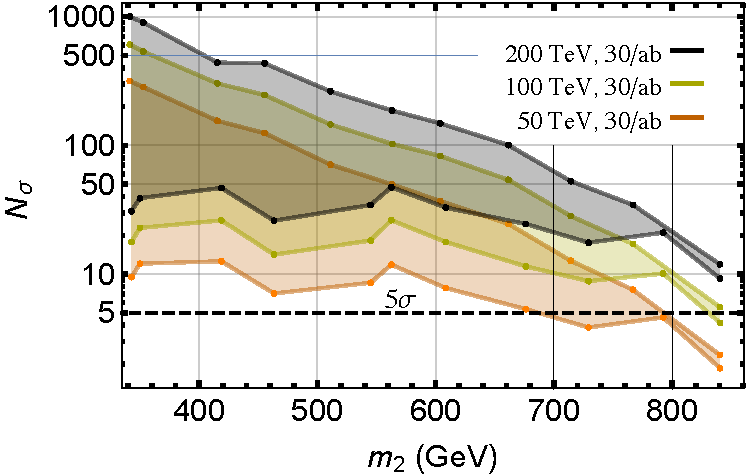
\includegraphics[width=0.49\linewidth]{\main/section3/plots/LogScale_Comb_bandPlot2.pdf}
    % 
    \caption{
    Discovery potential for the singlet-induced strong first order EWPT using resonant di-Higgs production combining 4\texttau\ and b\={b}\textgamma\textgamma\ final states\cite{Kotwal:2016tex}. Vertical axis gives significance as a function of the singlet-like scalar mass $m_2$. Left panel gives comparison of the reach for the HL-LHC (blue band) and the FCC-hh with 3 ab$^{-1}$ and 30 ab$^{-1}$ (purple and red bands, respectively). Right panel shows the prospective reach for different centre of mass energies, assuming 30 ab$^{-1}$.    
        }
    \label{fig:ewpt_resdihiggs}
  \end{center}
\end{figure}

It is worth noting that the foregoing analyses are based on the assumption that the di-Higgs production process is dominated by the resonant amplitude. As discussed in Section 9.6.2, inclusion of interference with non-resonant amplitudes may lead to an enhanced sensitivity, particularly at higher values of the singlet-like mass $m_2$. The corresponding gain in going to the HE-LHC may be as much as a 40-50\% increase in mass reach compared to that of the HL-LHC, depending on the choice of other model parameters.

Another class of signatures providing important information about the couplings in the Higgs potential in singlet-extended Higgs sectors involves pair production of the new scalar itself. These processes can complement resonant di-Higgs production in their coverage of the parameter space. For example, the process $p p\rightarrow h_2 h_2 \rightarrow 3\ell 3\nu j j$ was analysed in Ref.~\cite{Chen:2017qcz} and shown to provide good sensitivity to the first-order EWPT-compatible parameter space at both the high luminosity LHC and a future 100 \UTeV collider for masses below the di-Higgs threshold. While the analogous study has not been performed for the 27 \UTeV HE-LHC, $h_2 h_2$ production should still provide sensitivity to the couplings in the potential responsible for strengthening the EWPT, improving over the reach of the HL-LHC. In models in which a new $\mathbb{Z}_2$ symmetry is imposed on the singlet scalar, the VBF-like topology $p p \rightarrow j j h_2 h_2$ can be used to access the relevant Higgs portal coupling. In this case, $h_2$ is stable and escapes the detector as missing energy. Ref.~\cite{Curtin:2014jma} showed that this process at 100 \UTeV can probe first-order EWPTs for relatively low scalar masses. The analogous studies for the 14 \UTeV HL-LHC and 27 \UTeV HE-LHC remain to be done. 

Beyond direct production, the HE LHC will provide opportunities to observe indirect signatures of a strong first order EWPT through modifications of Higgs couplings. Considering first the xSM, the mixing between the doublet and singlet states will lead to modifications of the Higgs triple self coupling. This possibility is indicated in Fig.~\ref{fig:ewpt_self}, where we show he correlation between the critical temperature for the first order EWPT and the triple self coupling. The vertical axis gives the ratio of the xSM triple self-coupling of Higgs-like state $h_1$ to its Standard Model value, corresponding to the quantity $\kappa_\lambda$  introduced earlier in this chapter.  According to the analysis presented in the first part of Section~\ref{sec:THanetal}, a 15\% determination of $\kappa_\lambda$ may be possible using the $bb\gamma\gamma$ channel (however, see a parallel analysis later in that section for a less optimistic projection). This sensitivity corresponds roughly to the width of the green band in Fig.~\ref{fig:ewpt_self}. One can see that there exists a wide range of xSM parameter choices that would lead to an observable deviation of $\kappa_\lambda$ with the HE LHC.

\begin{figure}[hbtp]
  \begin{center}
    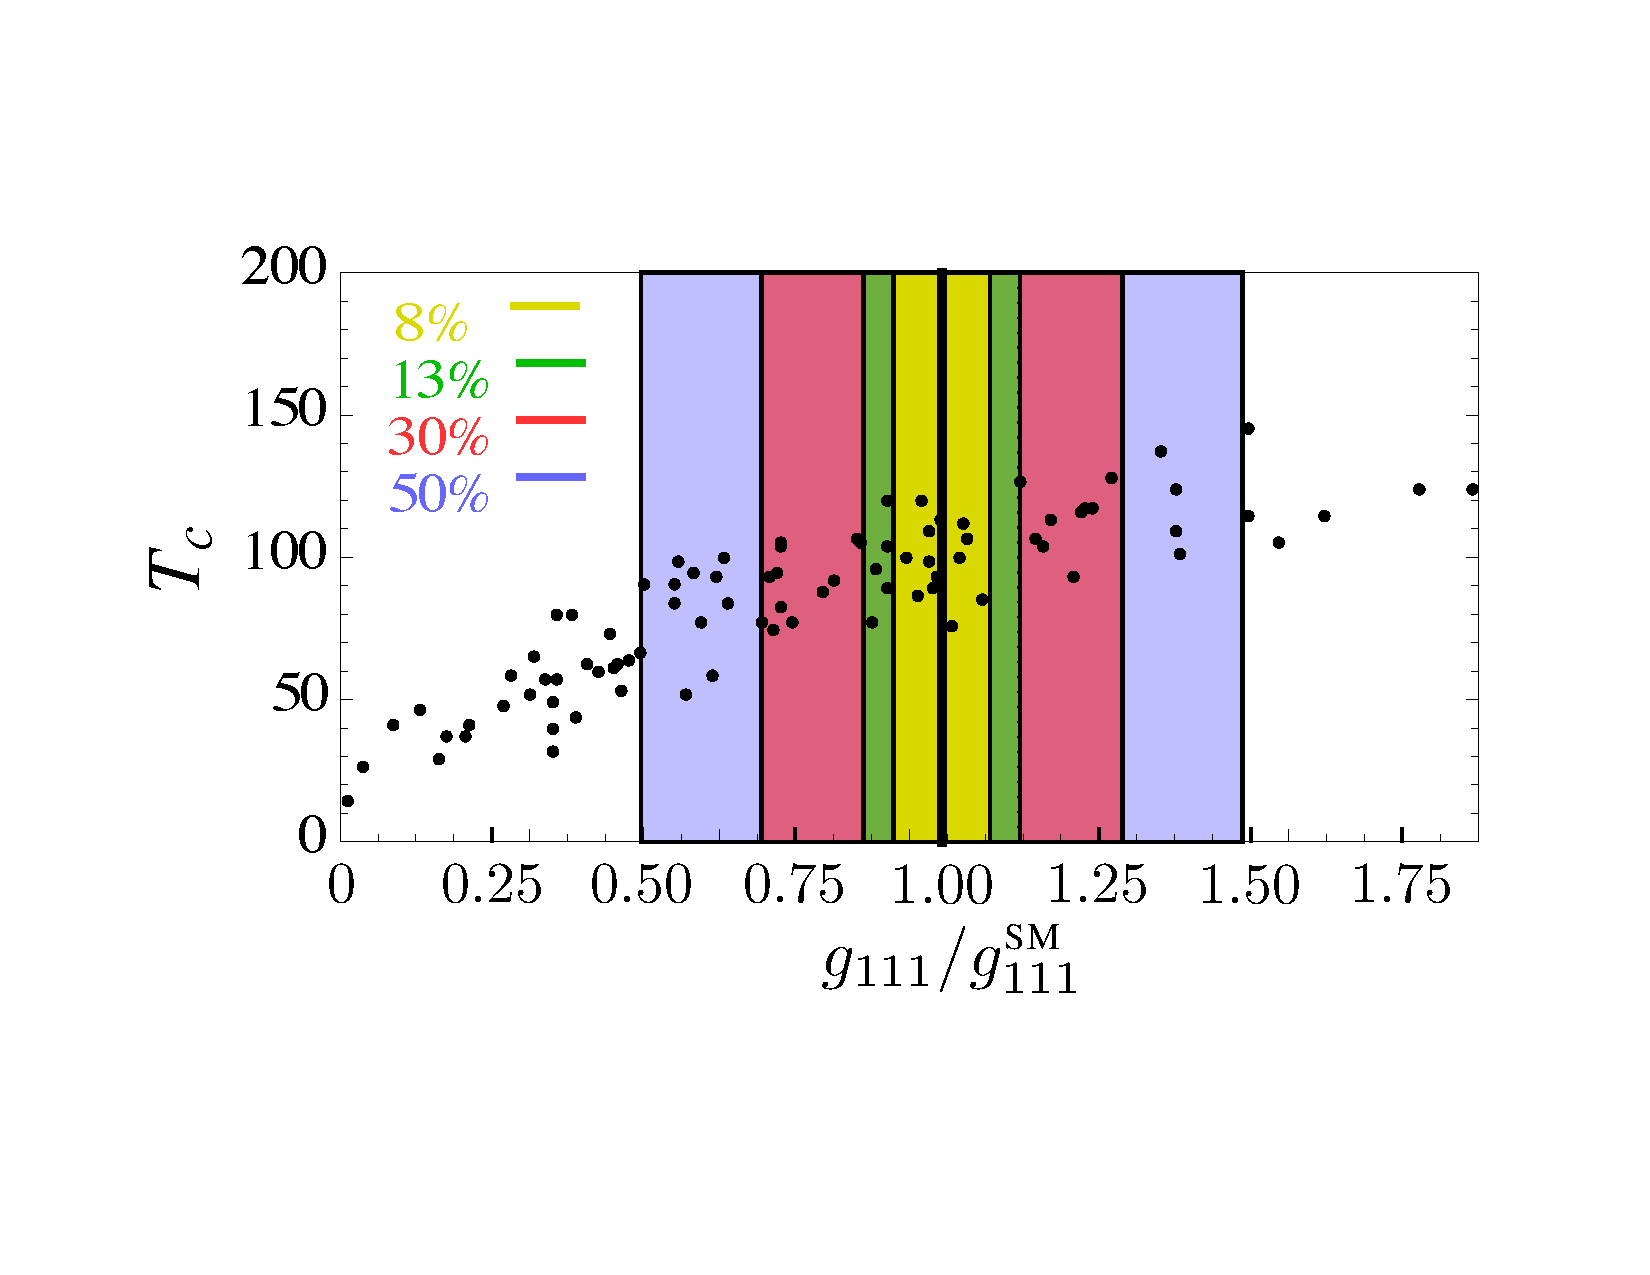
\includegraphics[width=0.49\linewidth]{\main/section3/plots/Self_Coupling--rescale_axis.pdf}
  %  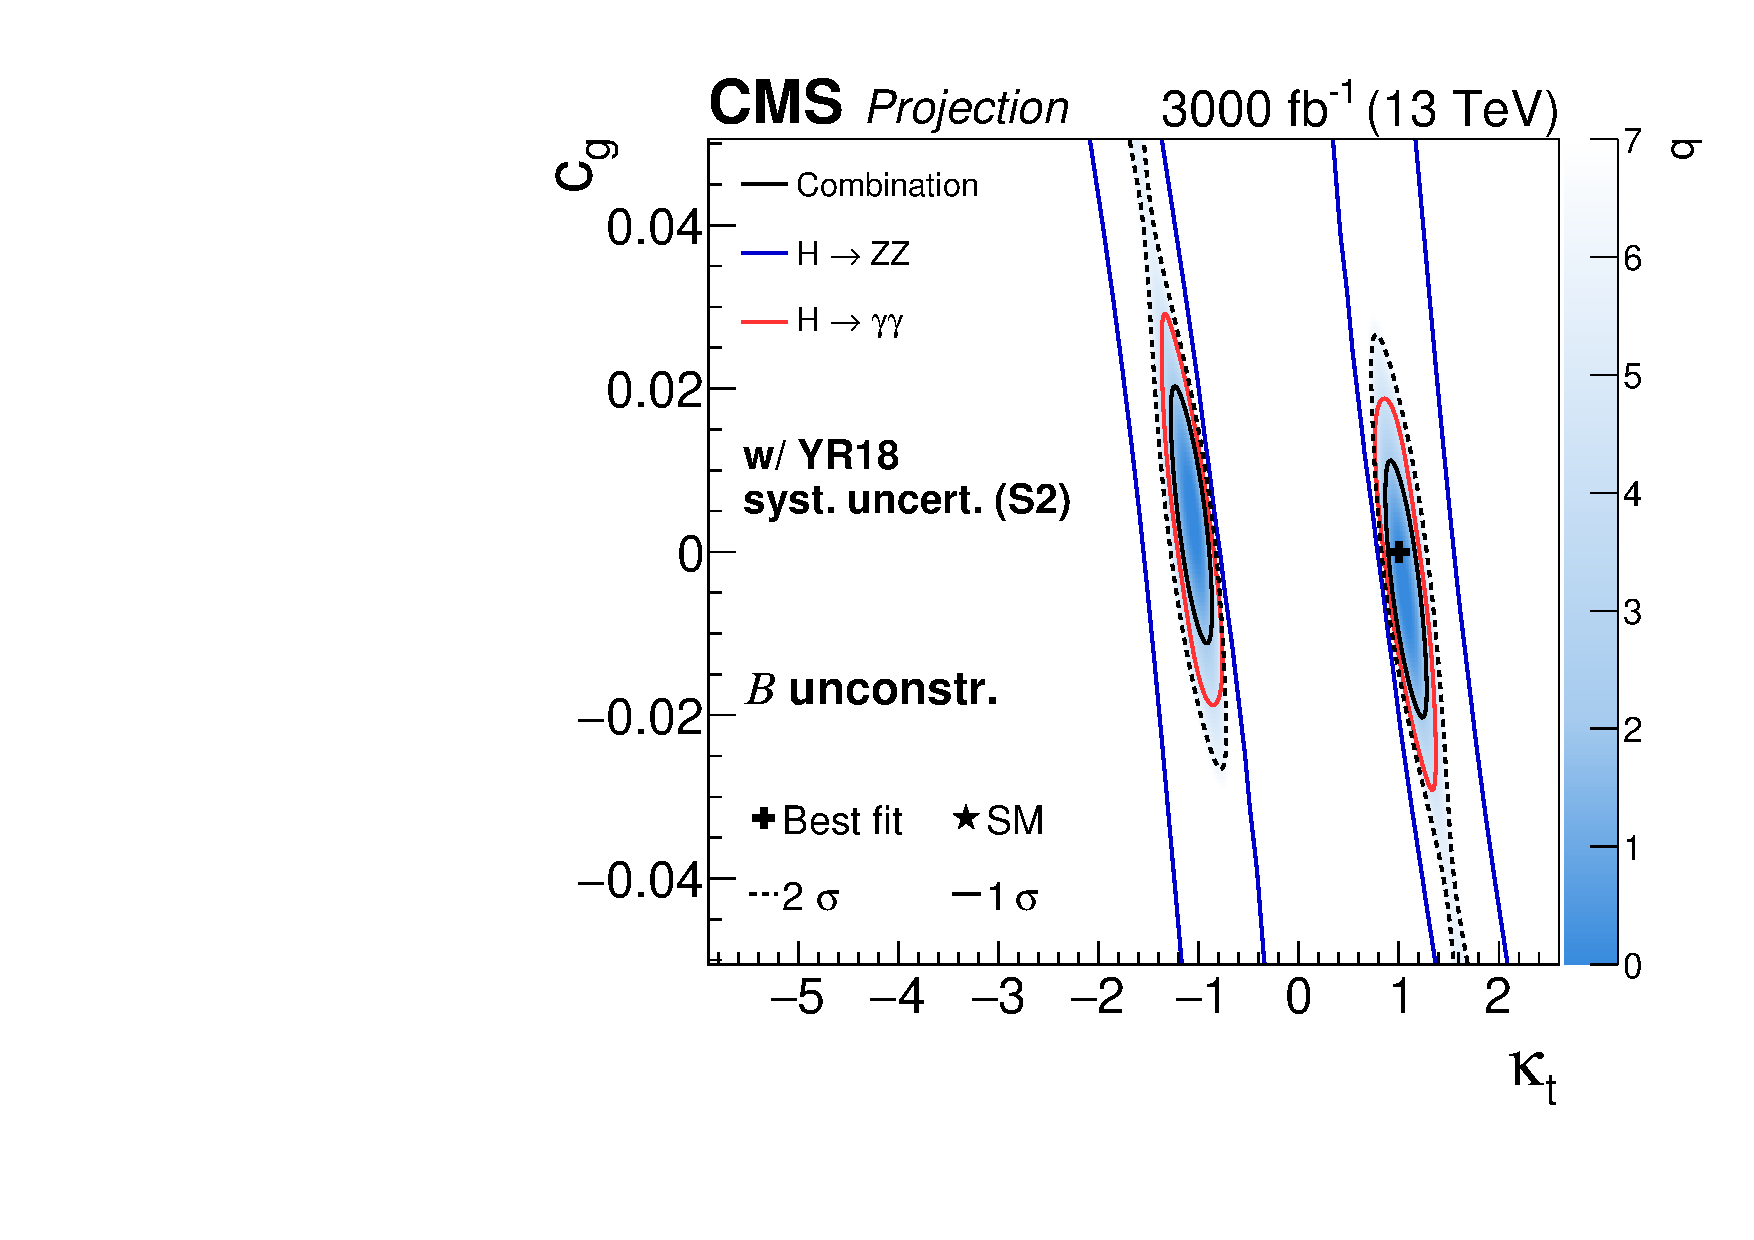
\includegraphics[width=0.49\linewidth]{\main/section2/plots/differentials/projection_ktcg_plot_floatingBRs_scenario2.pdf}
    % 
    \caption{
    Parameter space scan for a singlet model extension of the Standard Model. The points indicate a first order phase transition. These points lead to signals observable at future colliders. Shown is the correlation between critical temperature $T_c$ (vertical axis) and the triple Higgs ($h_1 h_1 h_1$) coupling scaled to its SM value (horizontal axis). SM prediction for the latter is indicated as $g_{111}/g_{111}^\mathrm{SM}=1$. Adapted from Ref.~\cite{Profumo:2014opa}   
        }
    \label{fig:ewpt_self}
  \end{center}
\end{figure}

\begin{figure}[hbtp]
  \begin{center}
  \includegraphics[width=0.49\linewidth]{\main/section3/plots/Triplet_EWPT.pdf}
    % 
    \caption{
    EW phase diagram for the real triplet extension of the SM scalar sector. Horizontal axis gives the triplet mass and vertical axis indicates the triplet-Higgs coupling. Light blue and green regions correspond to cross-over and first order transitions. Dark green (\lq\lq DR breaks down") and grey regions indicate parameter choices for which the present non-perturbative computations are not applicable. Dashed lines indicate relative shift $\delta$ in the Higgs di-photon decay rate compared to its Standard Model value. From Ref.~\cite{Niemi:2018asa}.    
        }
    \label{fig:ewpt_triplet}
  \end{center}
\end{figure}

Going beyond the SM, one may also anticipate a strong first order EWPT in scalar sector extensions carrying electroweak charge. Among the most widely studied ones, such scenario is the 2HDM. The authors of Refs.~~\cite{Dorsch:2013wja,Dorsch:2014qja} have shown that the strong phase transition would be correlated with the presence of the $\rm A^0\to Z H^0$ decay and that a nearly definitive probe of this possibility could be achieved with the LHC. An interesting alternative is a scalar EW triplet with vanishing hyper-charge.Interactions between the latter and the Standard Model doublet could lead to breaking of electroweak symmetry through either a single transition to the Higgs phase or through a succession of transitions\cite{Patel:2012pi}. Recently, the latter possibility has been explored in Ref.~\cite{Niemi:2018asa} using non-perturbative methods. In this work, it is shown how a precise measurement of the Higgs di-photon decay rate could probe the nature of the transition in this scenario. Fig.~\ref{fig:ewpt_triplet} illustrates this possibility. The horizontal and vertical axes give the triplet mass and coupling to the Higgs boson, respectively. The light blue and green regions correspond to a cross-over transition and first order phase transition, respectively. The dashed lines indicate the relative reduction in the Higgs di-photon decay rate relative to the prediction for the Standard Model. When combined with knowledge of the triplet mass, a precise measurement of the di-photon decay rate would indicate whether the transition is first order or crossover. As shown in Fig. 30, one expects to achieve a 1.8\% ($1\sigma$) determination of the Higgs-di-photon coupling parameter $\kappa_\gamma$ with the HL-LHC.
%For a 5$\sigma$ observation, a measurement of $\Gamma($H$\to$\textgamma\textgamma) at the anticipated FCC precision would be needed.







%%%%%%%%%%%%%%%%%%%%%%%%%%%%%%%%
%% SUMMARY
%%%%%%%%%%%%%%%%%%%%%%%%%%%%%%%%

\subsection{Summary}

A measurement of the Higgs self-coupling is not only one of the last corners of the SM to be experimentally tested, but also a particularly interesting one due to its important implications on our knowledge of the Higgs potential, and the direct implications on the nature of electroweak symmetry breaking, the stability of our universe's vacuum and the matter-antimatter asymmetry. In this chapter we presented a study on the capabilities of the HL-LHC and HE-LHC programs to elucidate on these fundamental questions.

The Higgs self-coupling appears at tree level in the production of Higgs boson pairs. The SM cross section for $pp\to \HH$ computed at full NLO precision is $32.88^{13.5\%}_{-12.5\%}\,\text{fb}$ at $\sqrt{s}=14\,\text{TeV}$ and $127.7^{11.5\%}_{-10.4\%}\,\text{fb}$ at $\sqrt{s}=27\,\text{TeV}$, a factor 4 increase between the two center of mass energies. The full NLO dependence on the trilinear coupling has been computed and illustrated in Table~\ref{tab:sigmatot} for selected coupling strength values. The NLO cross section has been computed for a set of benchmark points in the nonlinear EFT formalism as reported in Table~\ref{sigmatot}.

The ATLAS projections at HL-LHC for the $b\bar{b}b\bar{b}$, $b\bar{b}\tau\bar{\tau}$ and $b\bar{b}\gamma\gamma$ decay modes are summarized in Fig.~\ref{fig:ATLAS_HH_comb}. Considering the systematic uncertainties, the $b\bar{b}b\bar{b}$ channel gives the constraints $-2.3\leq \kappa_\lambda \leq 6.4$ at 68\% CL; the  $b\bar{b}\tau\bar{\tau}$ allows to resolve the region between the two minima giving $0.1\leq \kappa_\lambda\leq 2.3 \cup 5.7\leq \kappa_\lambda \leq 7.8$; and the $b\bar{b}\gamma\gamma$ gives the best precision with the interval $-0.2 \leq \kappa_\lambda \leq 2.5$.

The CMS projections include, on top of the channels studied by ATLAS, the decays $b\bar{b}\ell\nu\ell\nu$ and $b\bar{b}\ell\ell\ell\ell$, with projected constraints $-1.7\leq \kappa_\lambda \leq 9.6$ and $-1.8\leq \kappa_\lambda \leq 8.1$ respectively. For the other channels, the projected reach is $-0.6\leq \kappa_\lambda \leq 7.2$ for $b\bar{b}b\bar{b}$, $-0.2\leq \kappa_\lambda \leq 3.2 \cup 5.2\leq \kappa_\lambda \leq 7.7$ for  $b\bar{b}\tau\bar{\tau}$ and $0.3\leq \kappa_\lambda \leq 2.3$ for $b\bar{b}\gamma\gamma$.

Experiments provide a combination of the projections, summarized in Fig~\ref{fig:comb_HH_experiment} and Fig.~\ref{fig:comb_HH}. A combined significance of $4\sigma$ for the SM \HH signal is predicted.
The 68\% CL intervals are $0.52\leq \kappa_\lambda \leq 1.5$ and $0.57\leq \kappa_\lambda \leq 1.5$ with and without systematic uncertainties respectively. The second minimum is excluded at 99.4\% CL, and the hypothesis corresponding to the absence of self-coupling  ($\kappa_\lambda=0$) is excluded at the 95\% CL.

Further improvements in the analysis are proposed. The Topness and Higgsness variables can further increase the signal sensitivity for $\HH$ production, and improved multivariate methods are proposed to improve the background discrimination in the $b\bar{b}\gamma\gamma$ channel.

For the future HE-LHC upgrade, ATLAS presented projections for the $b\bar{b}b\bar{b}$ and $b\bar{b}\tau\bar{\tau}$ channels, with an expected sensitivity of around 10\%-20\% on $\kappa_\lambda$.

A complementary strategy to exctract the trilinear from the LHC data consists in considering NLO corrections to single Higgs observables that depend on the self-coupling. This dependence has been computed and is presented in Tables~\ref{c1s},\ref{tab:c1-xs_13},\ref{tab:c1-xs_27},\ref{c1g}. The CMS experiment has provided a first analysis based on this strategy using $t\bar{t}\text{H}$ production with the decay $\text{H}\to \gamma\gamma$, with a resulting constraint of $-2\leq \kappa_\lambda\leq 5.5$, see Fig.~\ref{fig:ttHdiff_CMS_klambda_scan}. Considering that other parameters may affect single Higgs process, this has been studied under the perspective of a global fit, presented in Fig.~\ref{fig:hllhcchi2} estimating a $-3\leq \kappa_\lambda \leq 3$ reach at 68\% CL, complementing the constraints from double Higgs boson production. At HE-LHC, the projections are presented in Fig.~\ref{fig:helhcchi2}.

Implications of the $\HH$ measurements involve a wide variety of models. We present the interpretation within a flavour model which implies large Yukawa couplings for the light quarks, modifying the di-Higgs invariant mass distribution non-trivially, see Fig.~\ref{fig:hhflavourxsanddistr}. Also, Higgs boson pair production plays a crucial role on understanding the nature of the electroweak symmetry breaking phase transition, which might imply potentially observable effects if there are new states modifying the potential so that the matter-antimatter asymmetry can be explained via electroweak baryogenesis.


\begin{figure}[h]
  \centering
    \includegraphics[width=0.9\textwidth]{\main/section3/plots/tril_summaryplot.pdf}
\caption{Summary plot for the different constraints on the Higgs boson self-coupling $\kappa_\lambda$ at HL-LHC and at HE-LHC. \textbf{$bbWW$ MISSING}}
\label{fig:tril_summaryplot}
\end{figure}

\end{document}